\clearpage
\begin{apendicesenv}
\partapendices

\chapter{Galeria do Front-end}
\label{app:frontend}

Este apêndice reúne capturas em alta resolução da interface operacional do \textit{G-FShield}. A intenção é mostrar a navegação, os painéis analíticos e as telas administrativas sem poluir o fluxo principal da dissertação.
As imagens foram organizadas por função de uso para deixar clara a progressão da interface, desde a autenticação até as telas de comparação, monitoramento e administração.

\section{Acesso e Visão Geral}

As primeiras telas apresentam o ponto de entrada da plataforma e o painel inicial, que resumem o estado geral do sistema logo após a autenticação.
As Figuras~\ref{fig:app-front-sign-in} e~\ref{fig:app-front-overview} mostram essa passagem entre acesso e visão consolidada.

\begin{figure}[!htb]
  \centering
  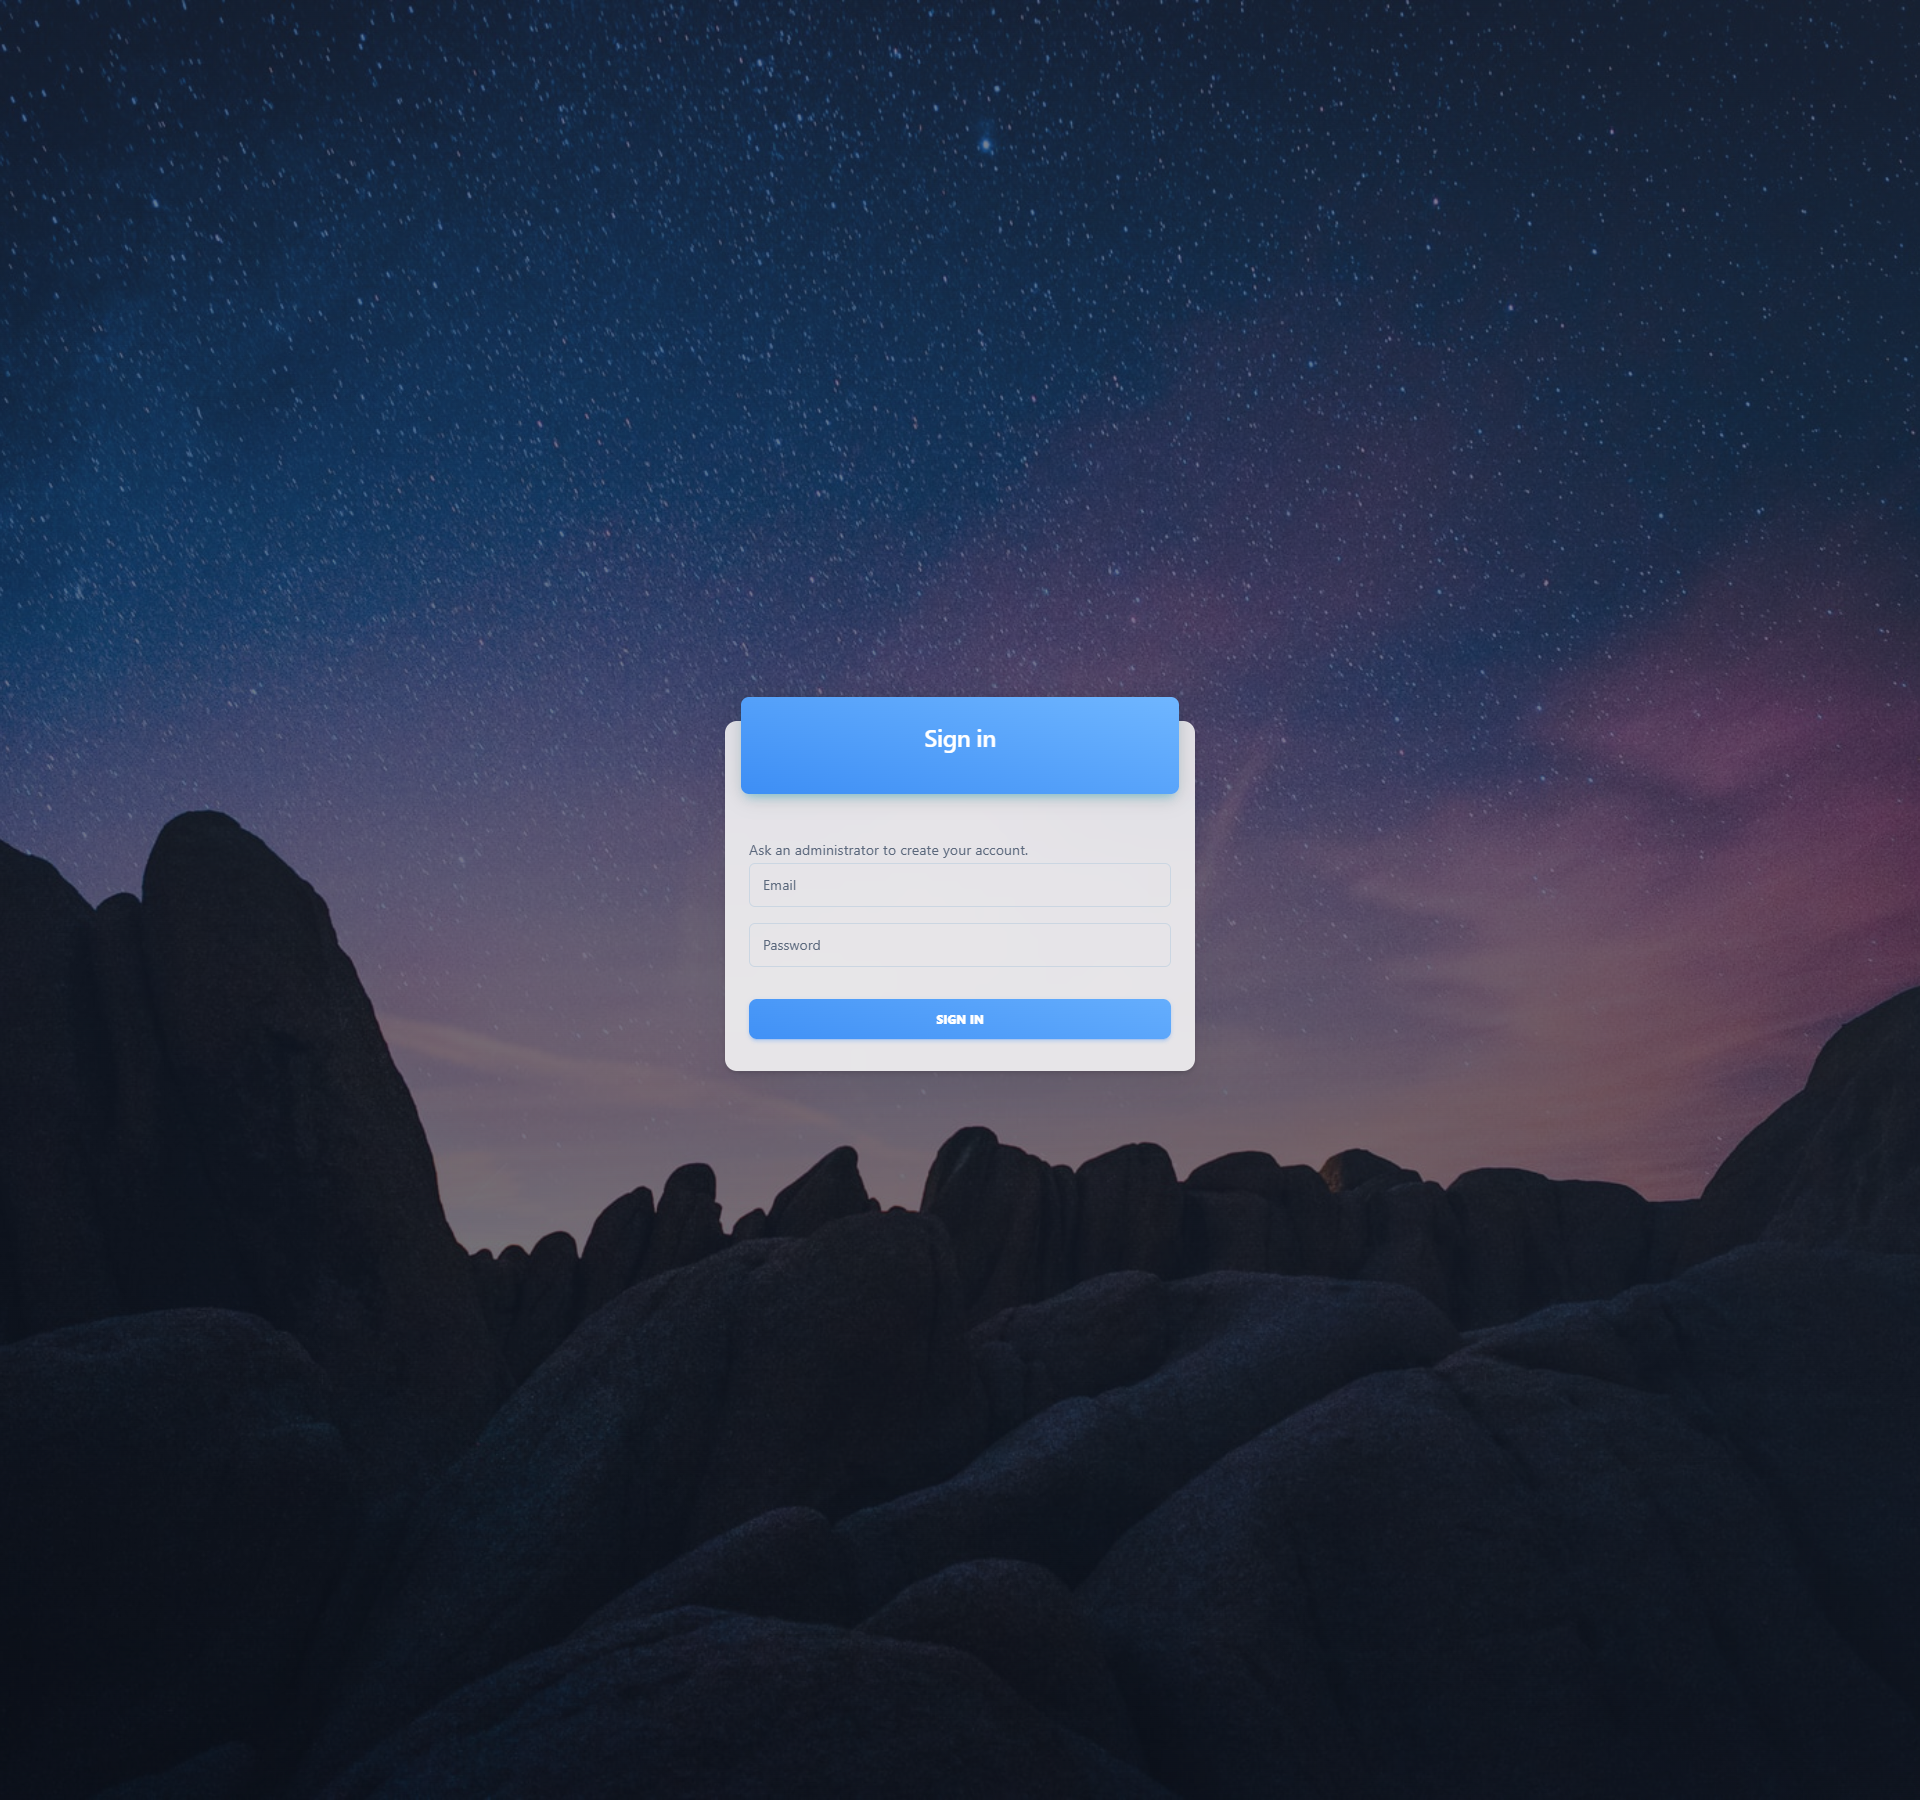
\includegraphics[width=\linewidth,height=0.80\textheight,keepaspectratio]{fig/front/00-sign-in.png}
  \caption{Tela de autenticação.}
  \label{fig:app-front-sign-in}
\end{figure}

\begin{figure}[!htb]
  \centering
  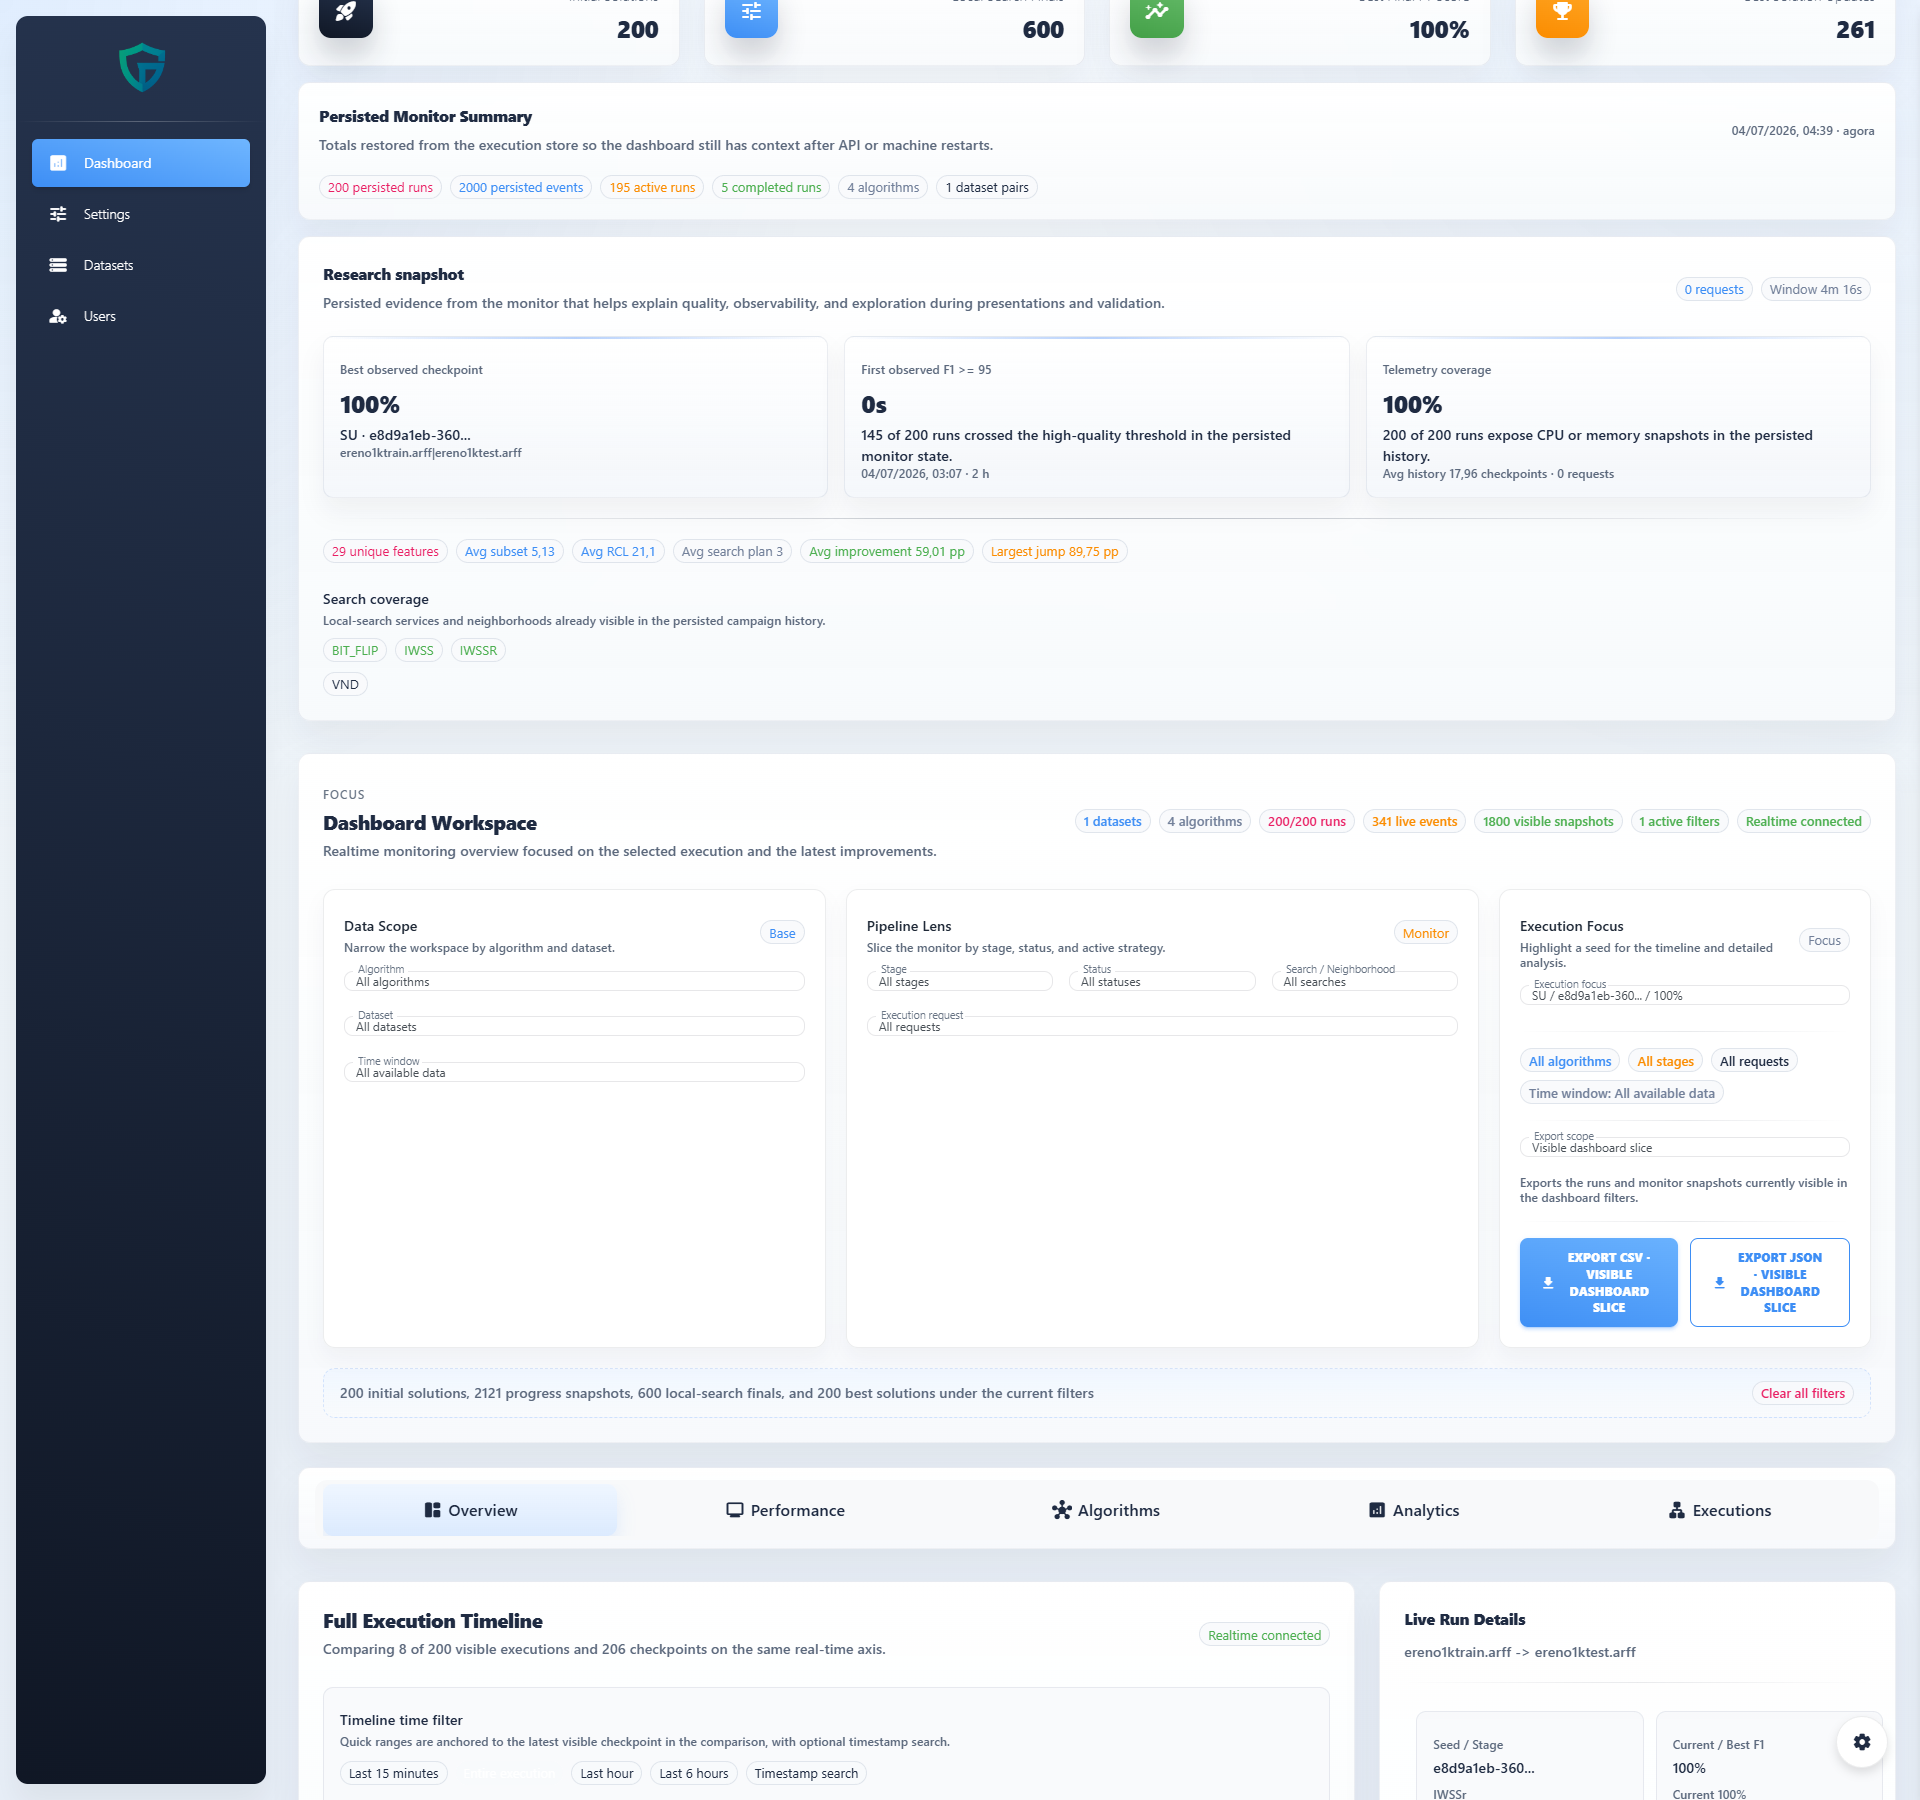
\includegraphics[width=\linewidth,height=0.80\textheight,keepaspectratio]{fig/front/01-dashboard-overview.png}
  \caption{Painel de visão geral.}
  \label{fig:app-front-overview}
\end{figure}

\clearpage
\section{Performance e Algoritmos}

Esta seção mostra como o usuário navega entre os painéis de desempenho e de comparação algorítmica, o que é importante para demonstrar a leitura operacional do sistema.
As Figuras~\ref{fig:app-front-performance} e~\ref{fig:app-front-algorithms} detalham essa leitura.

\begin{figure}[!htb]
  \centering
  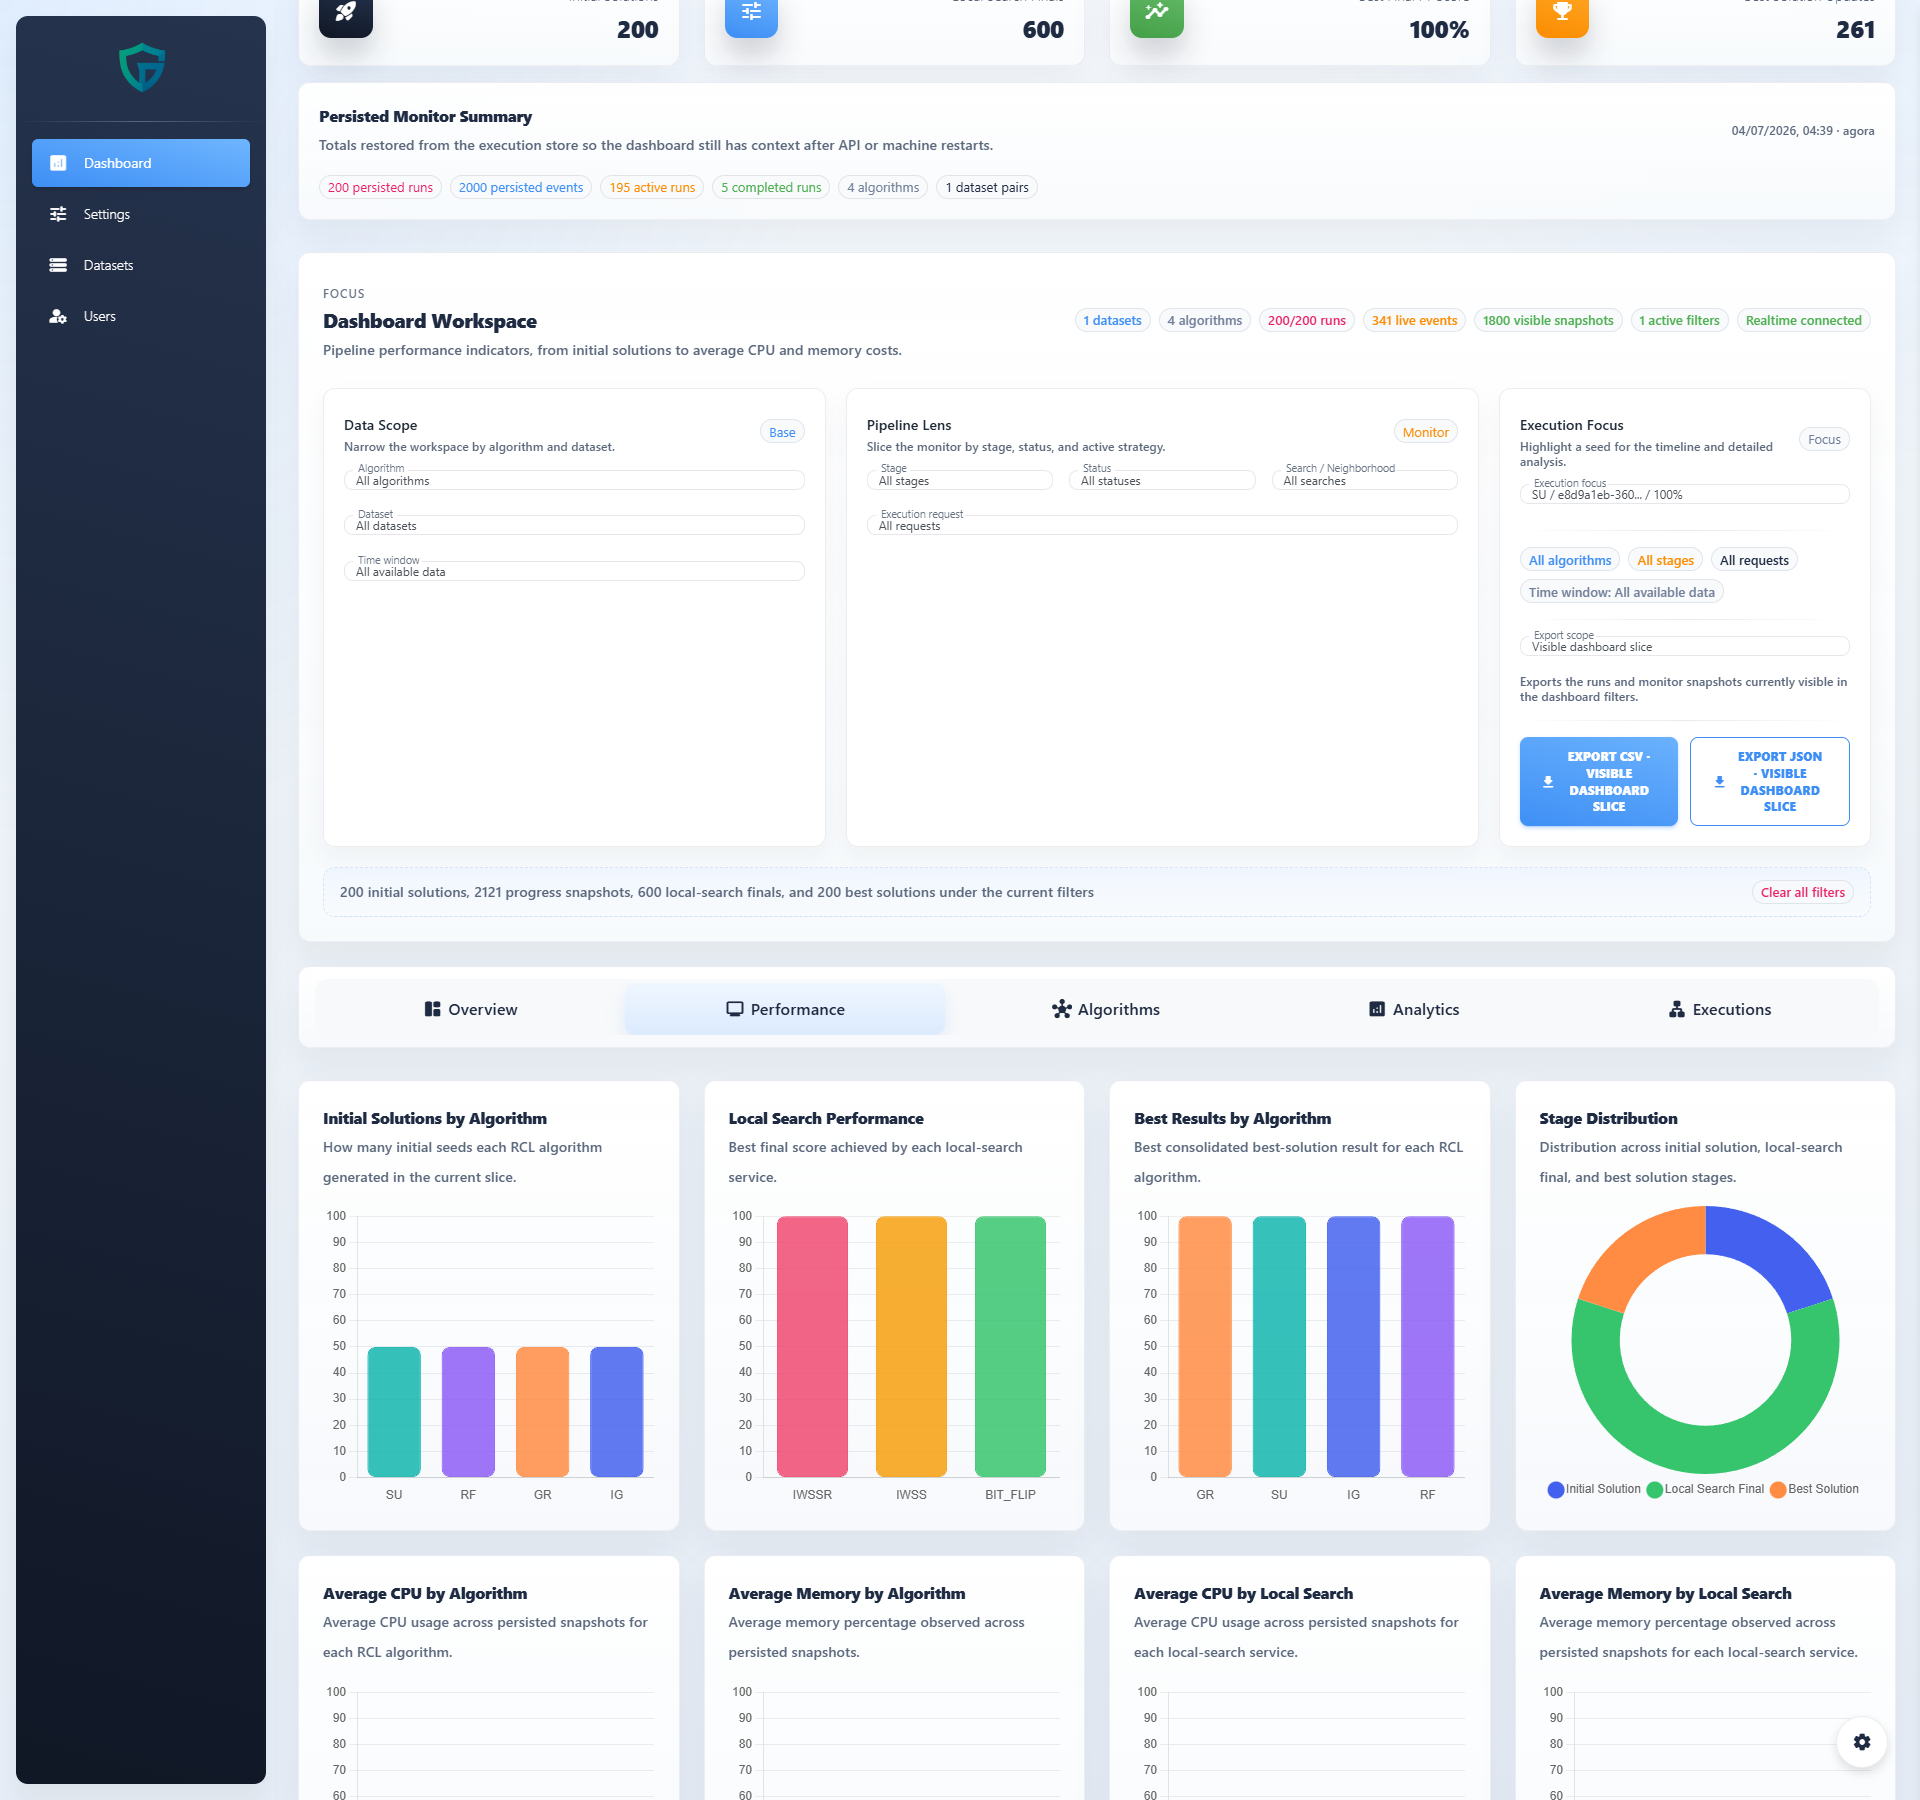
\includegraphics[width=\linewidth,height=0.80\textheight,keepaspectratio]{fig/front/02-dashboard-performance.png}
  \caption{Tela de performance.}
  \label{fig:app-front-performance}
\end{figure}

\begin{figure}[!htb]
  \centering
  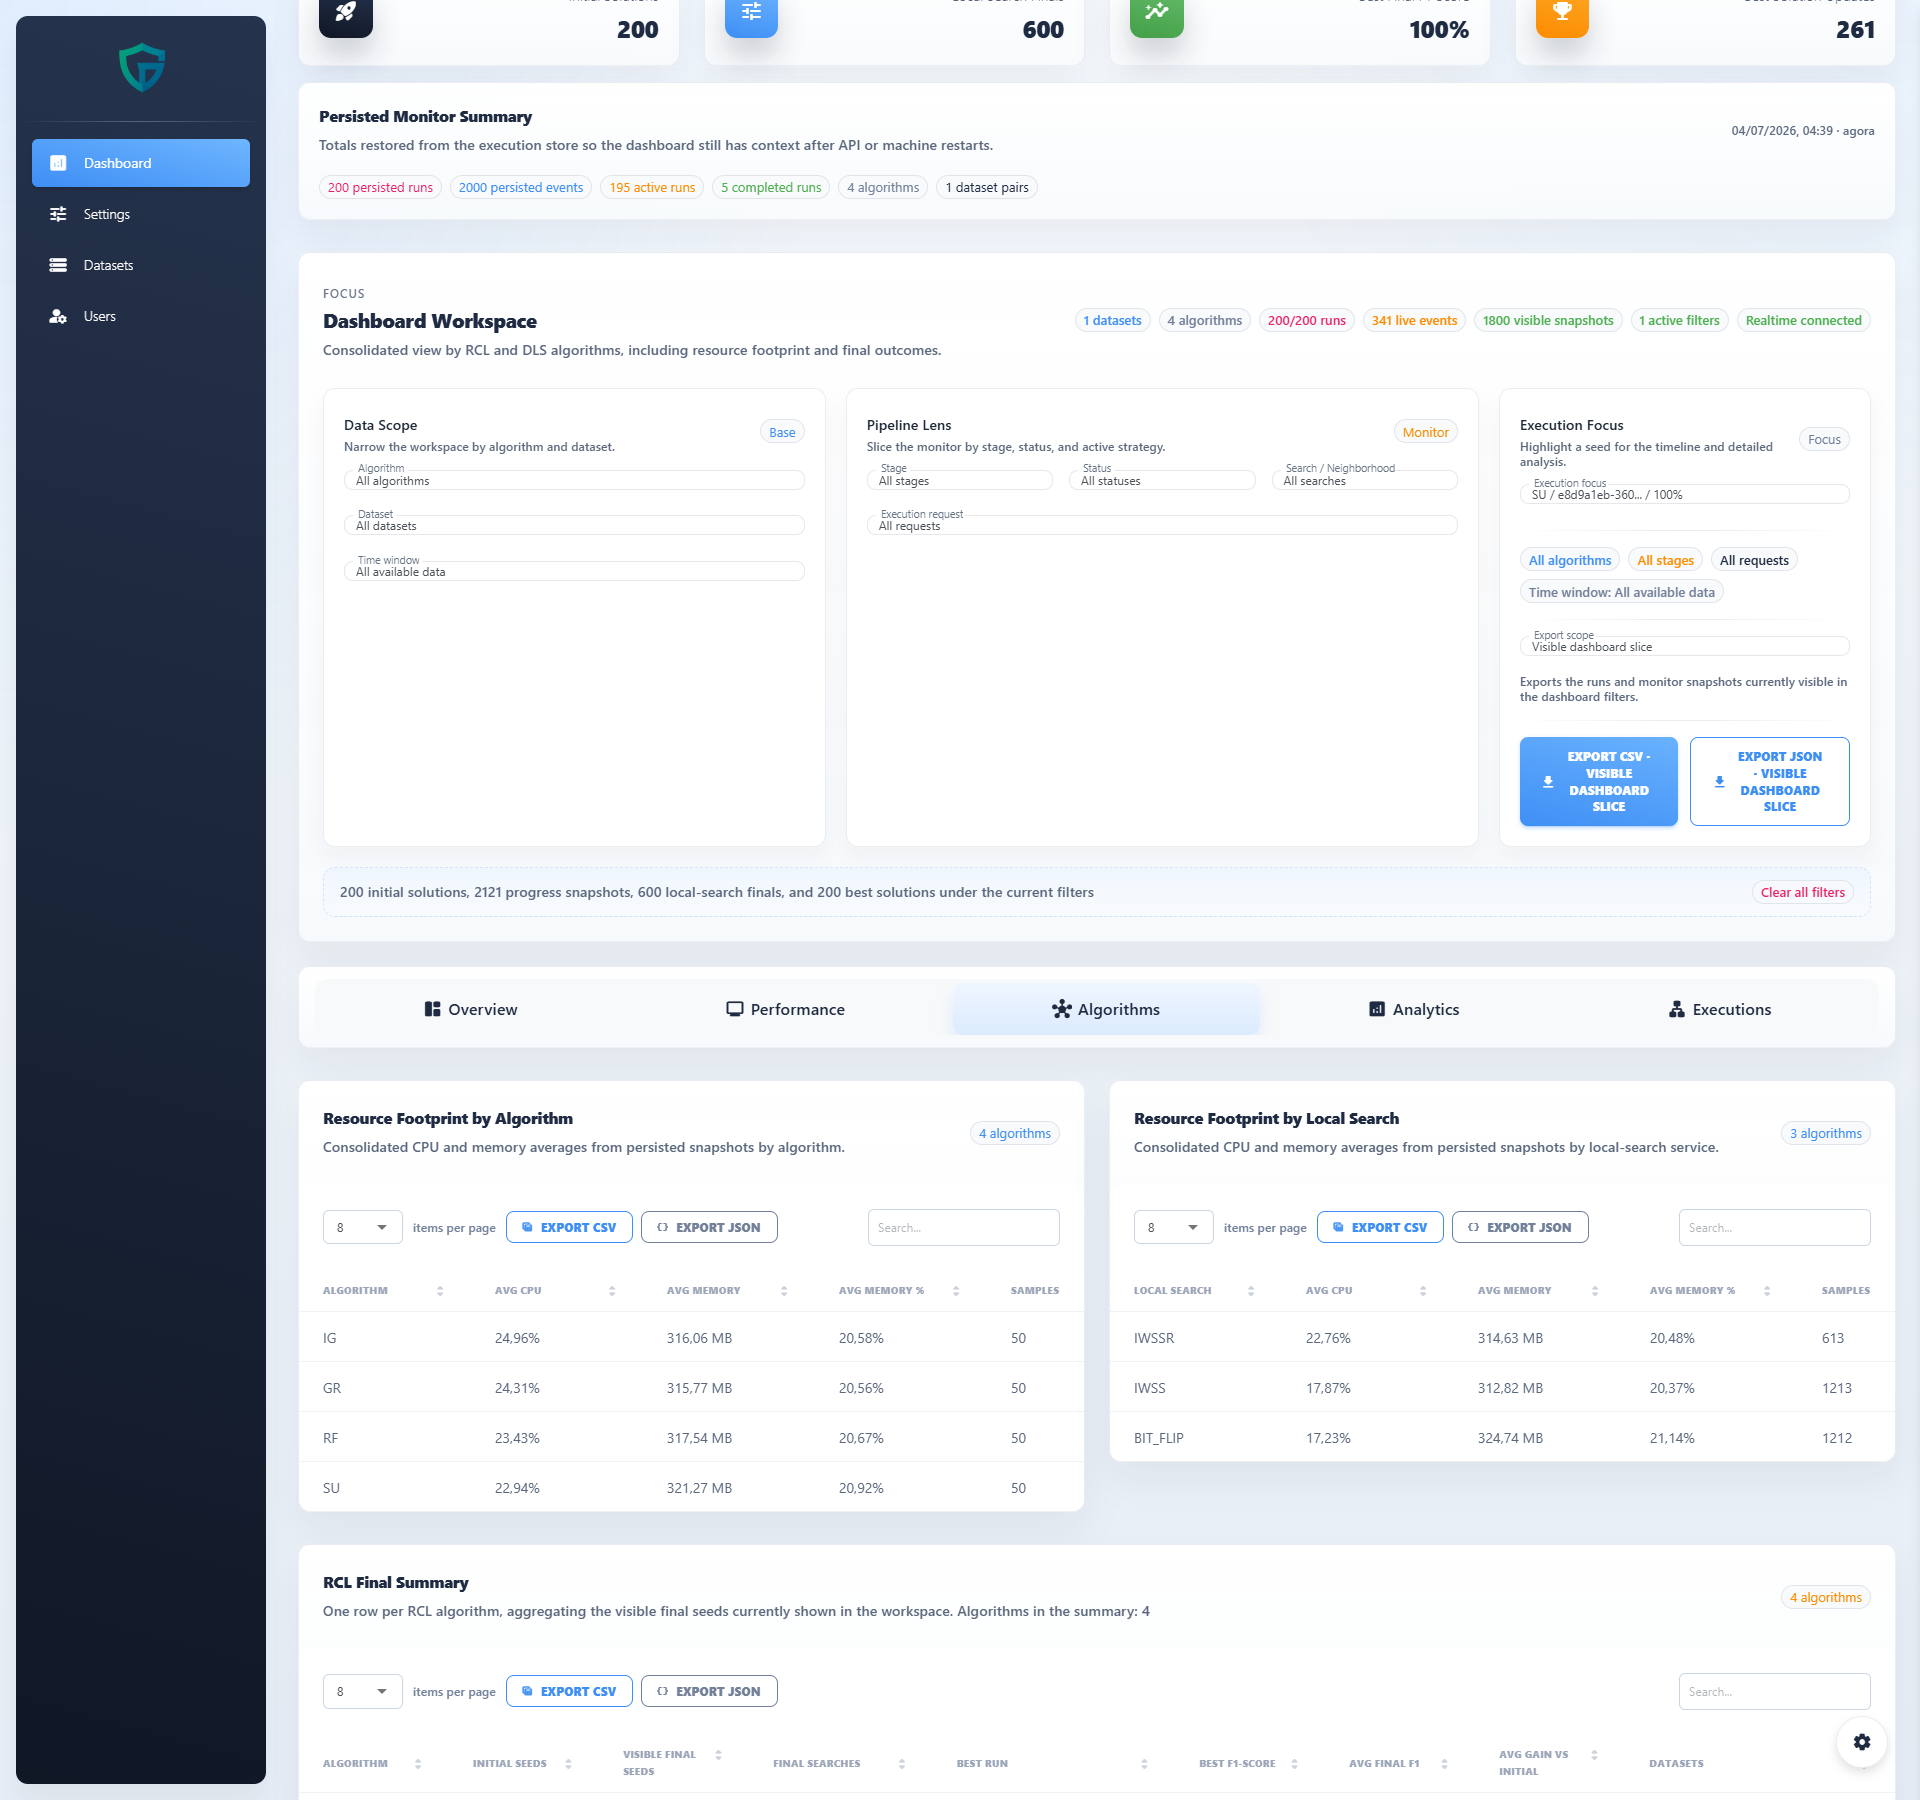
\includegraphics[width=\linewidth,height=0.80\textheight,keepaspectratio]{fig/front/03-dashboard-algorithms.png}
  \caption{Tela de comparação de algoritmos.}
  \label{fig:app-front-algorithms}
\end{figure}

\clearpage
\section{Analytics}

Os painéis analíticos resumem a atividade de execução e ajudam a observar tendências agregadas, detalhes por evento e tópicos persistidos.
As Figuras~\ref{fig:app-front-analytics-activity},~\ref{fig:app-front-analytics-activity-detail},~\ref{fig:app-front-analytics-topics} e~\ref{fig:app-front-analytics-feed} organizam essa visão em camadas.

\begin{figure}[!htb]
  \centering
  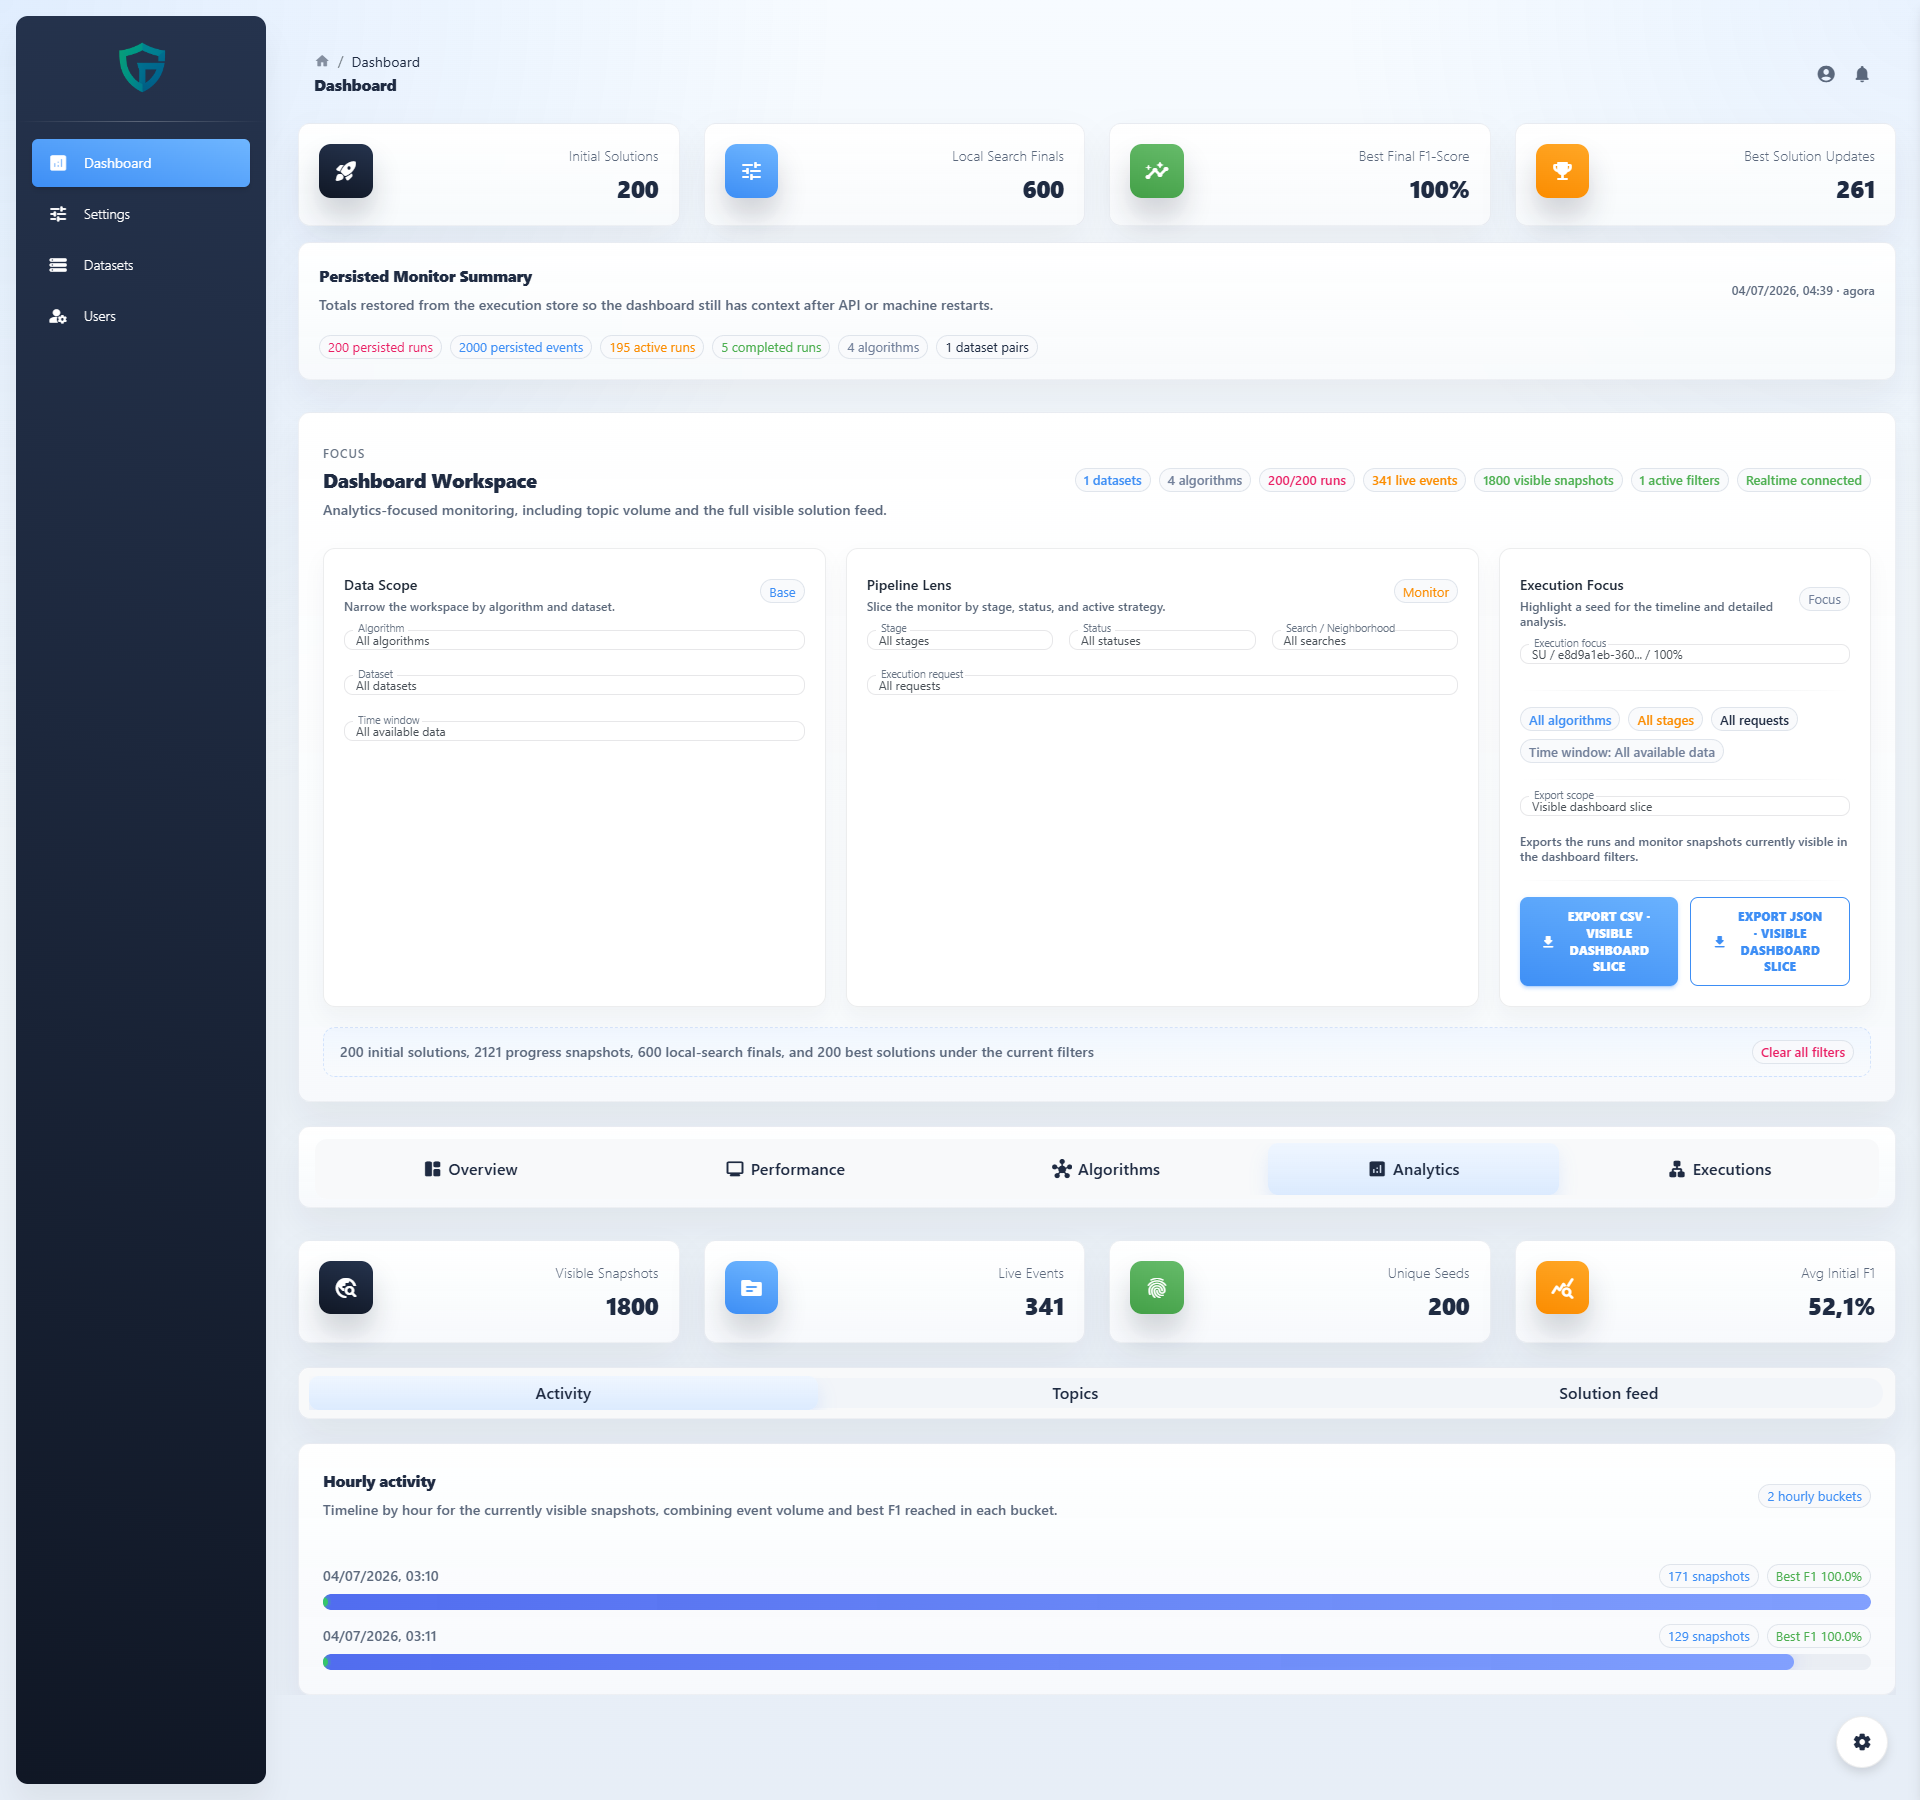
\includegraphics[width=\linewidth,height=0.80\textheight,keepaspectratio]{fig/front/04-dashboard-analytics-activity.png}
  \caption{Atividade analítica agregada.}
  \label{fig:app-front-analytics-activity}
\end{figure}

\begin{figure}[!htb]
  \centering
  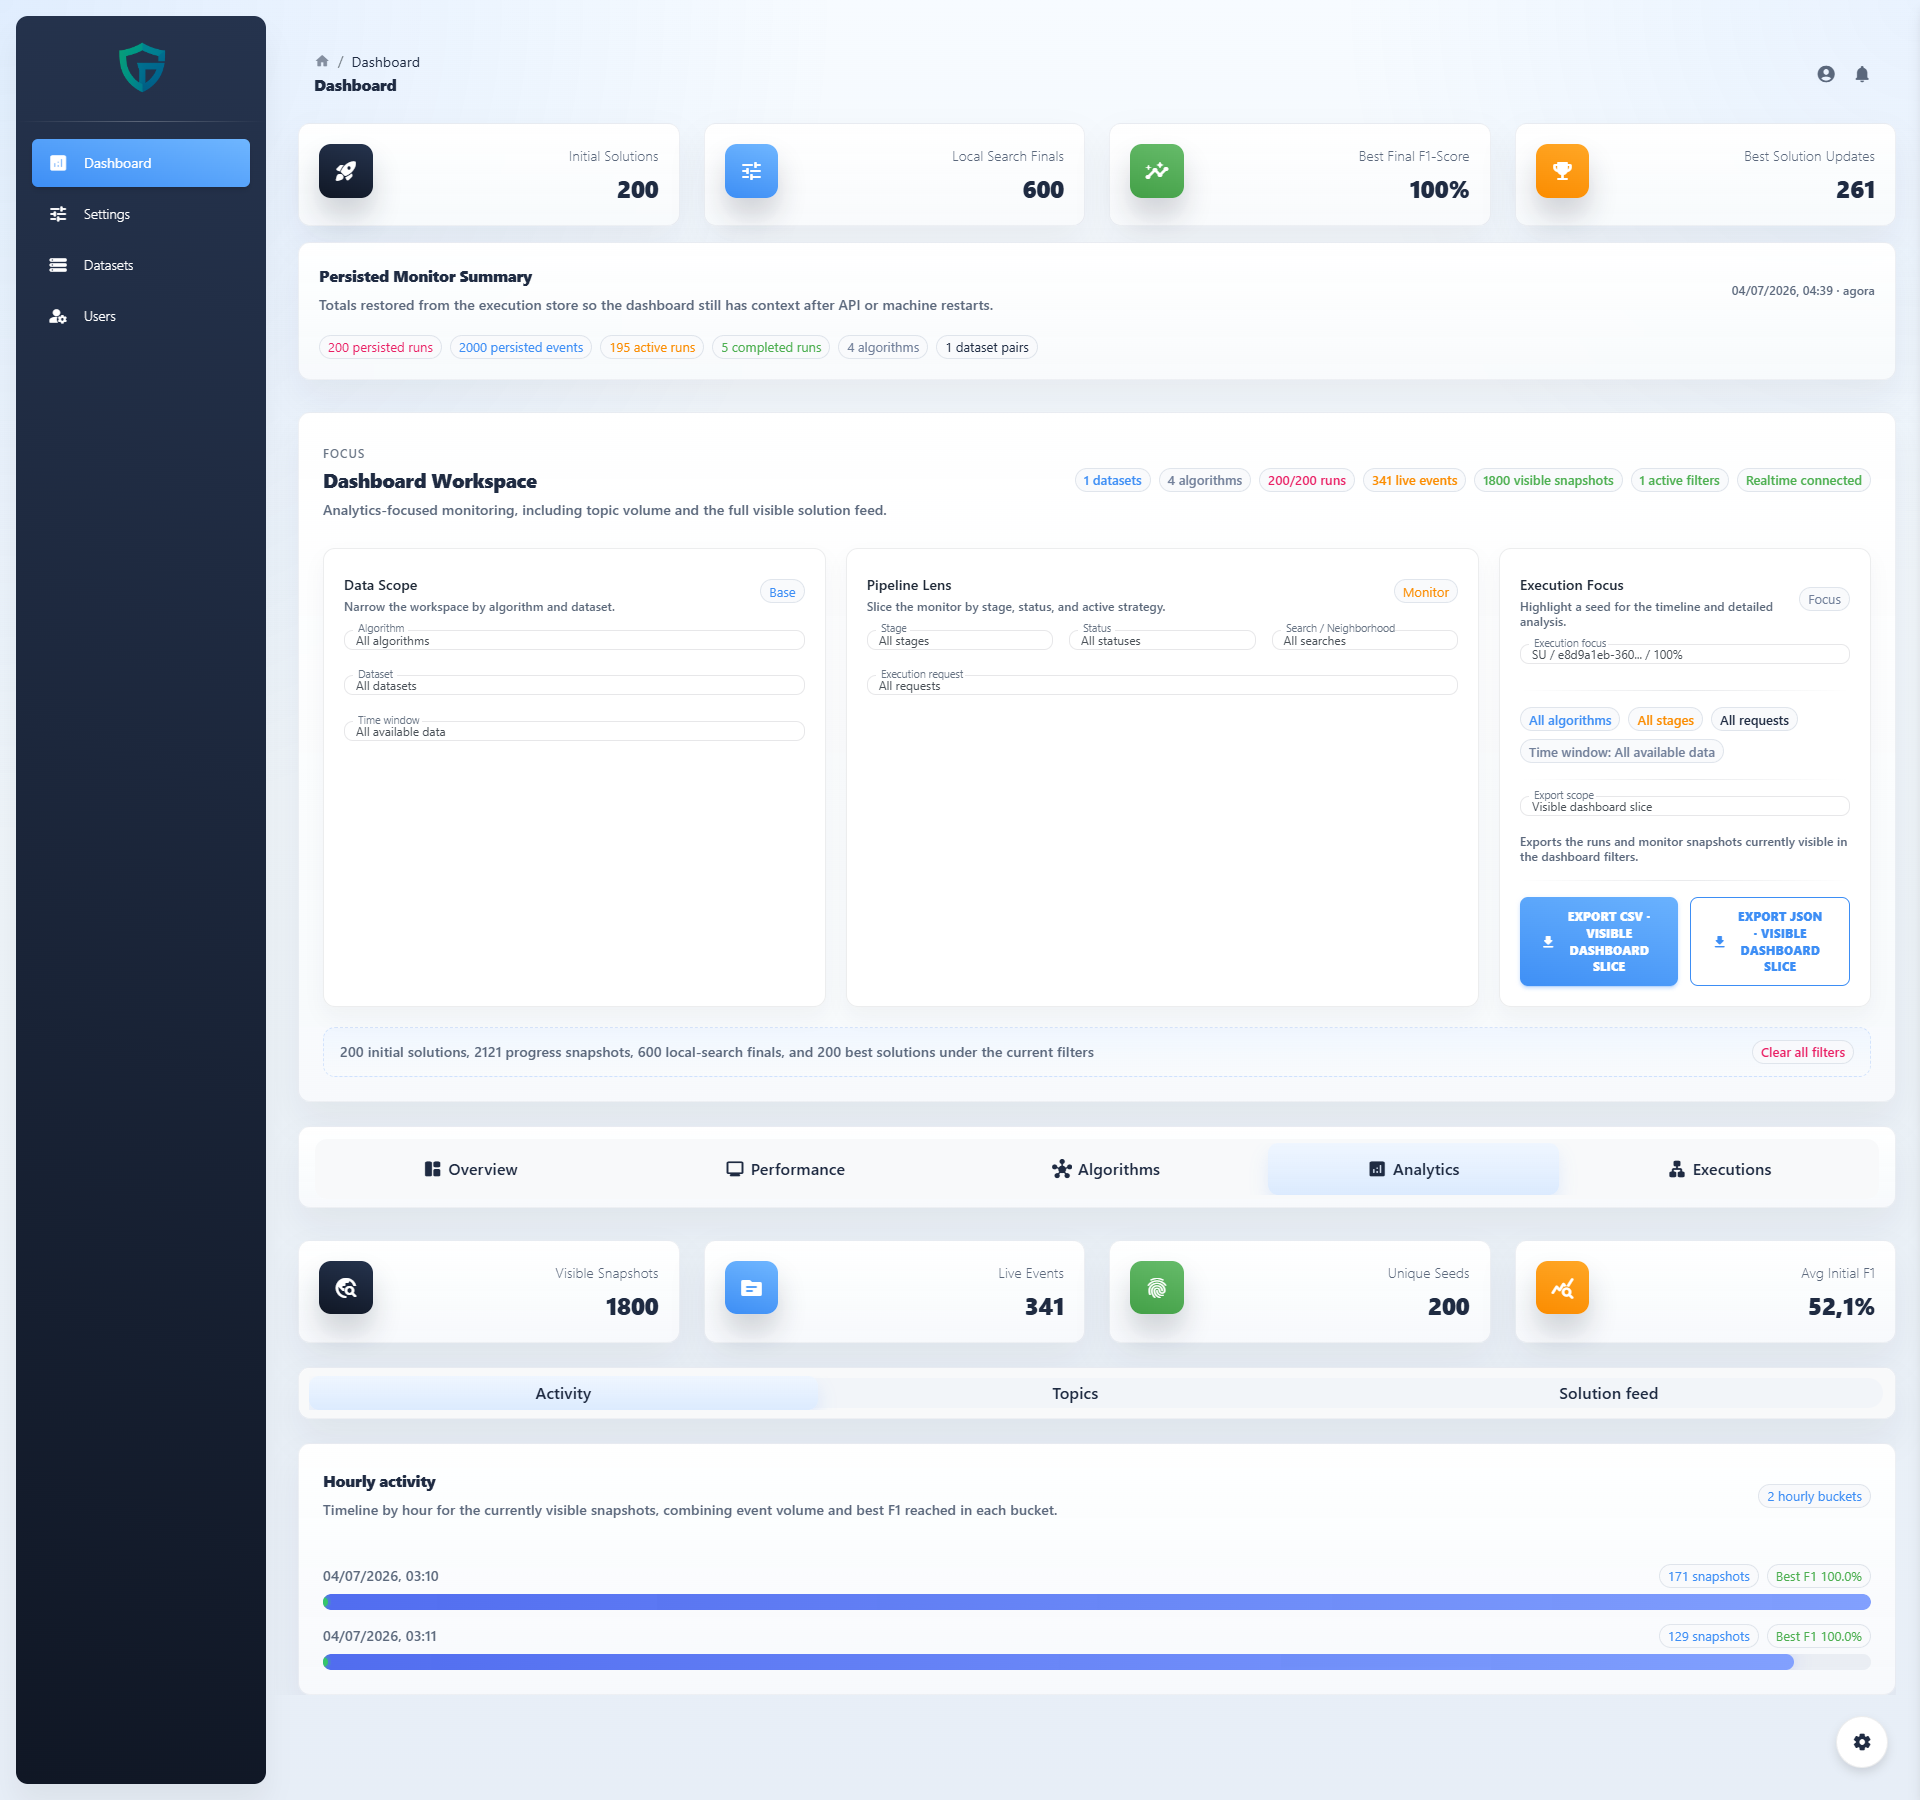
\includegraphics[width=\linewidth,height=0.80\textheight,keepaspectratio]{fig/front/05-dashboard-analytics-activity-detail.png}
  \caption{Detalhe da atividade analítica.}
  \label{fig:app-front-analytics-activity-detail}
\end{figure}

\begin{figure}[!htb]
  \centering
  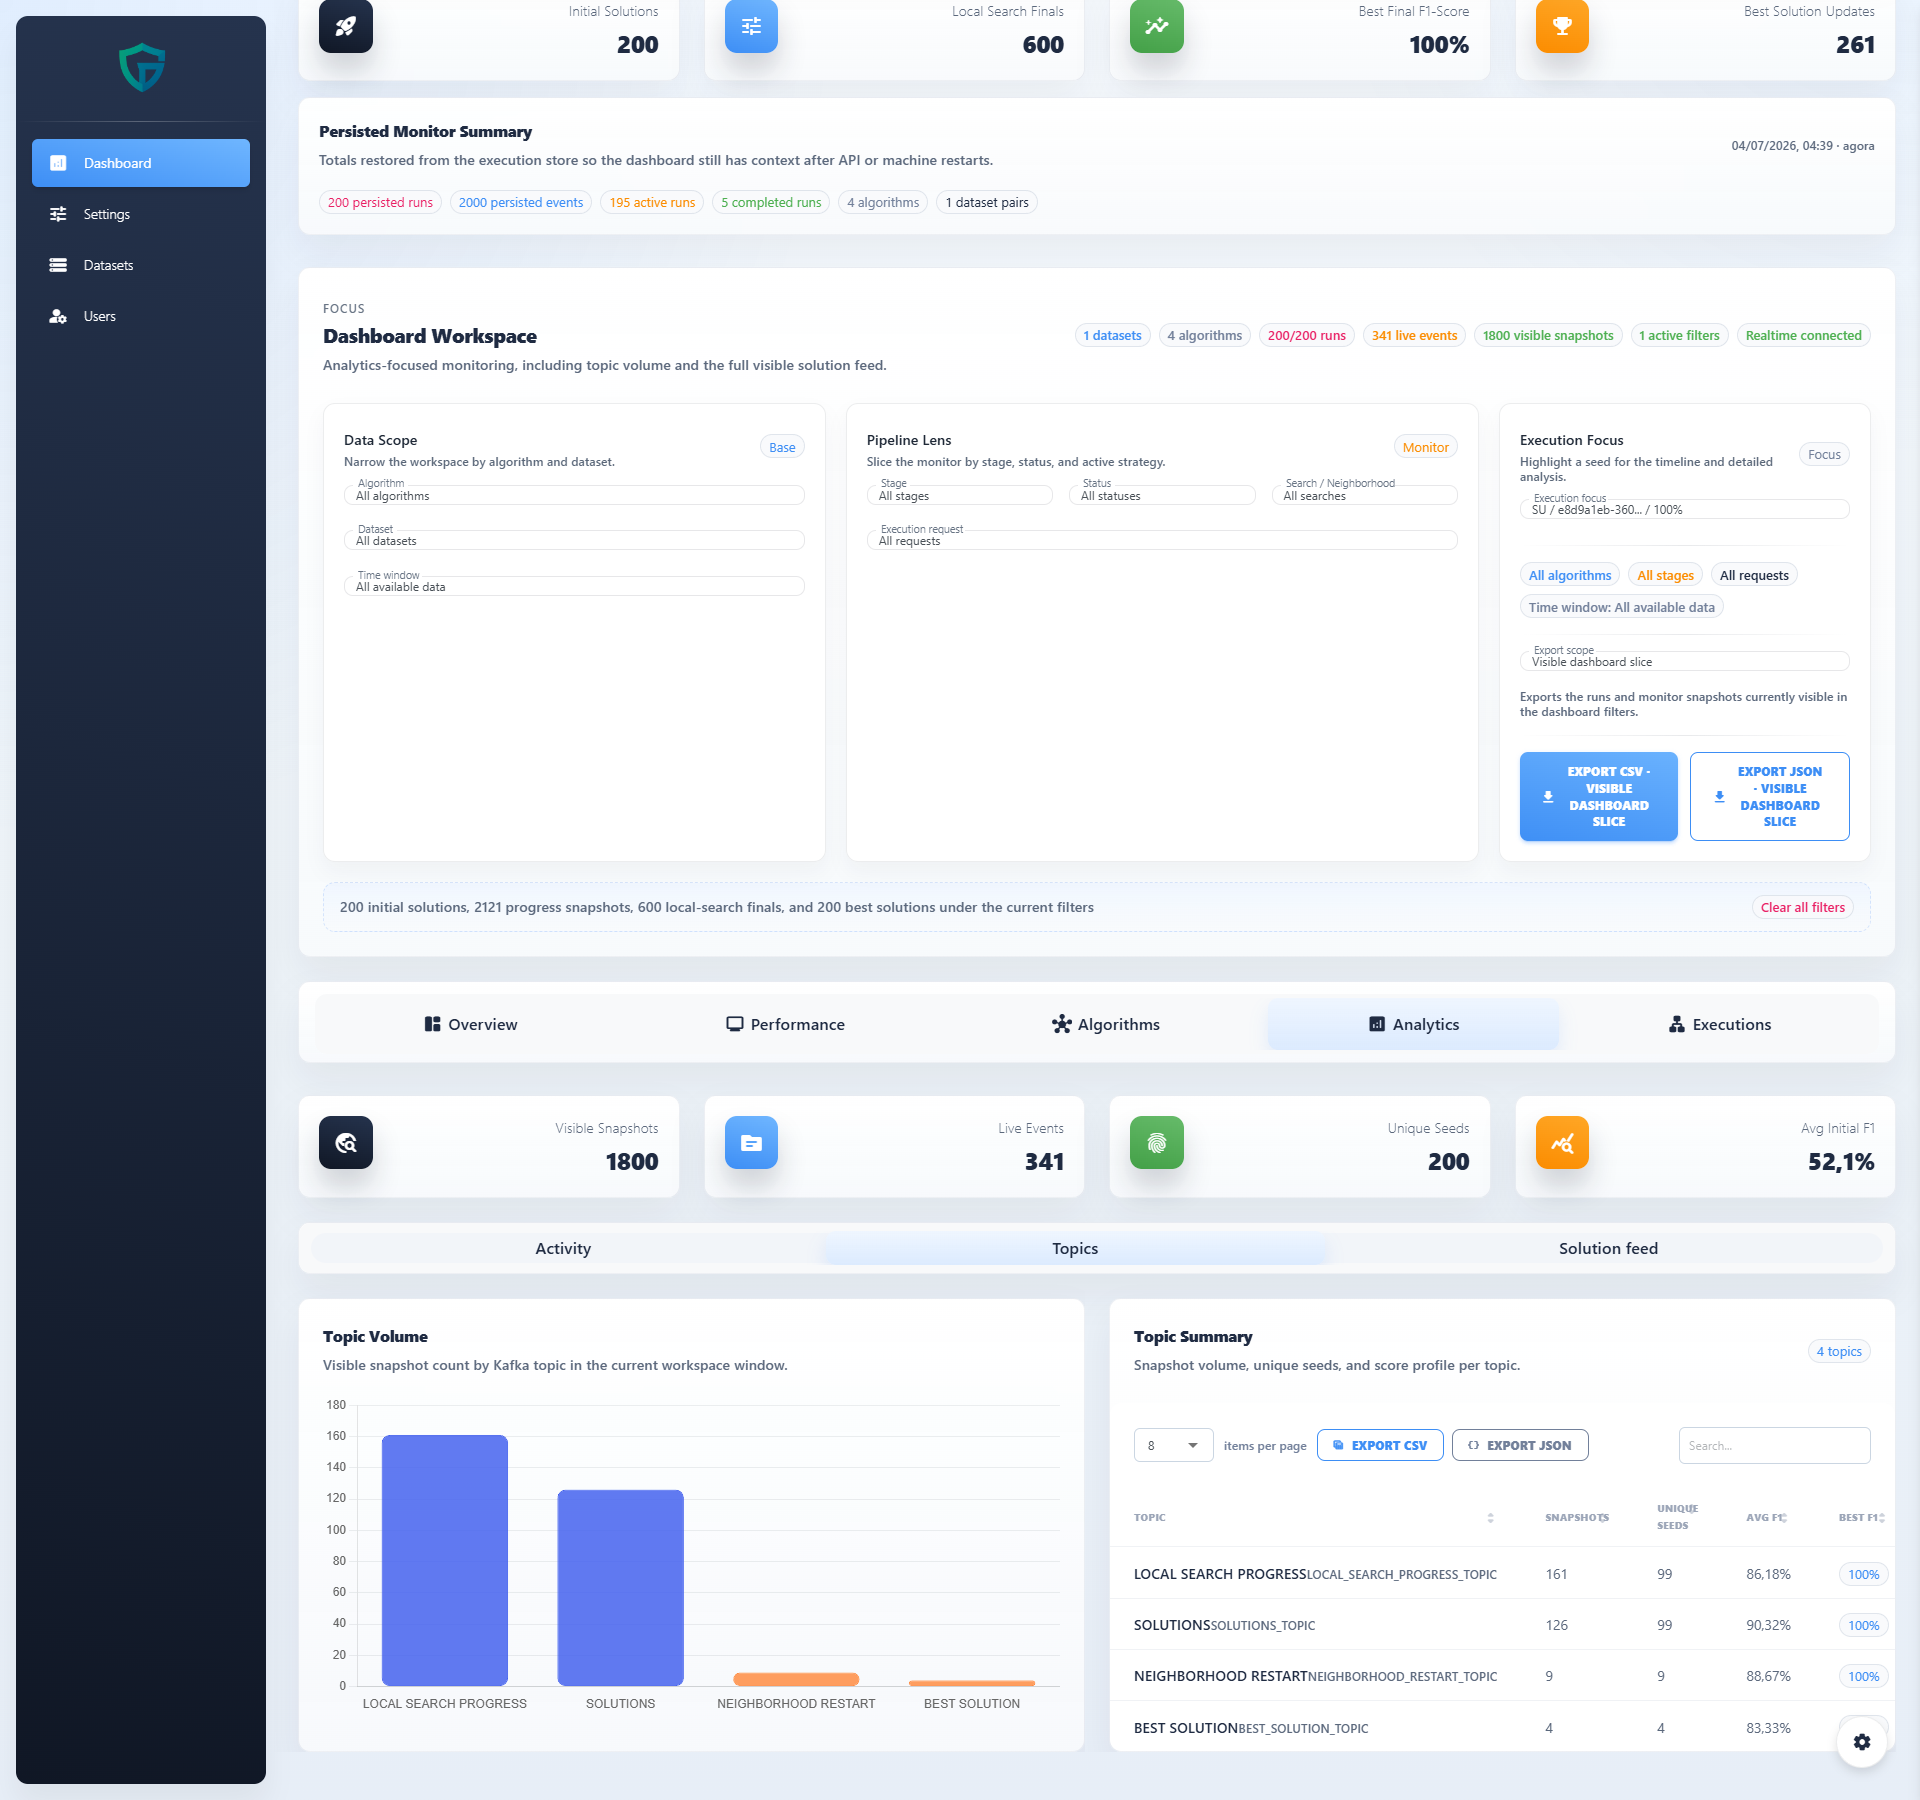
\includegraphics[width=\linewidth,height=0.80\textheight,keepaspectratio]{fig/front/06-dashboard-analytics-topics.png}
  \caption{Tópicos analíticos.}
  \label{fig:app-front-analytics-topics}
\end{figure}

\begin{figure}[!htb]
  \centering
  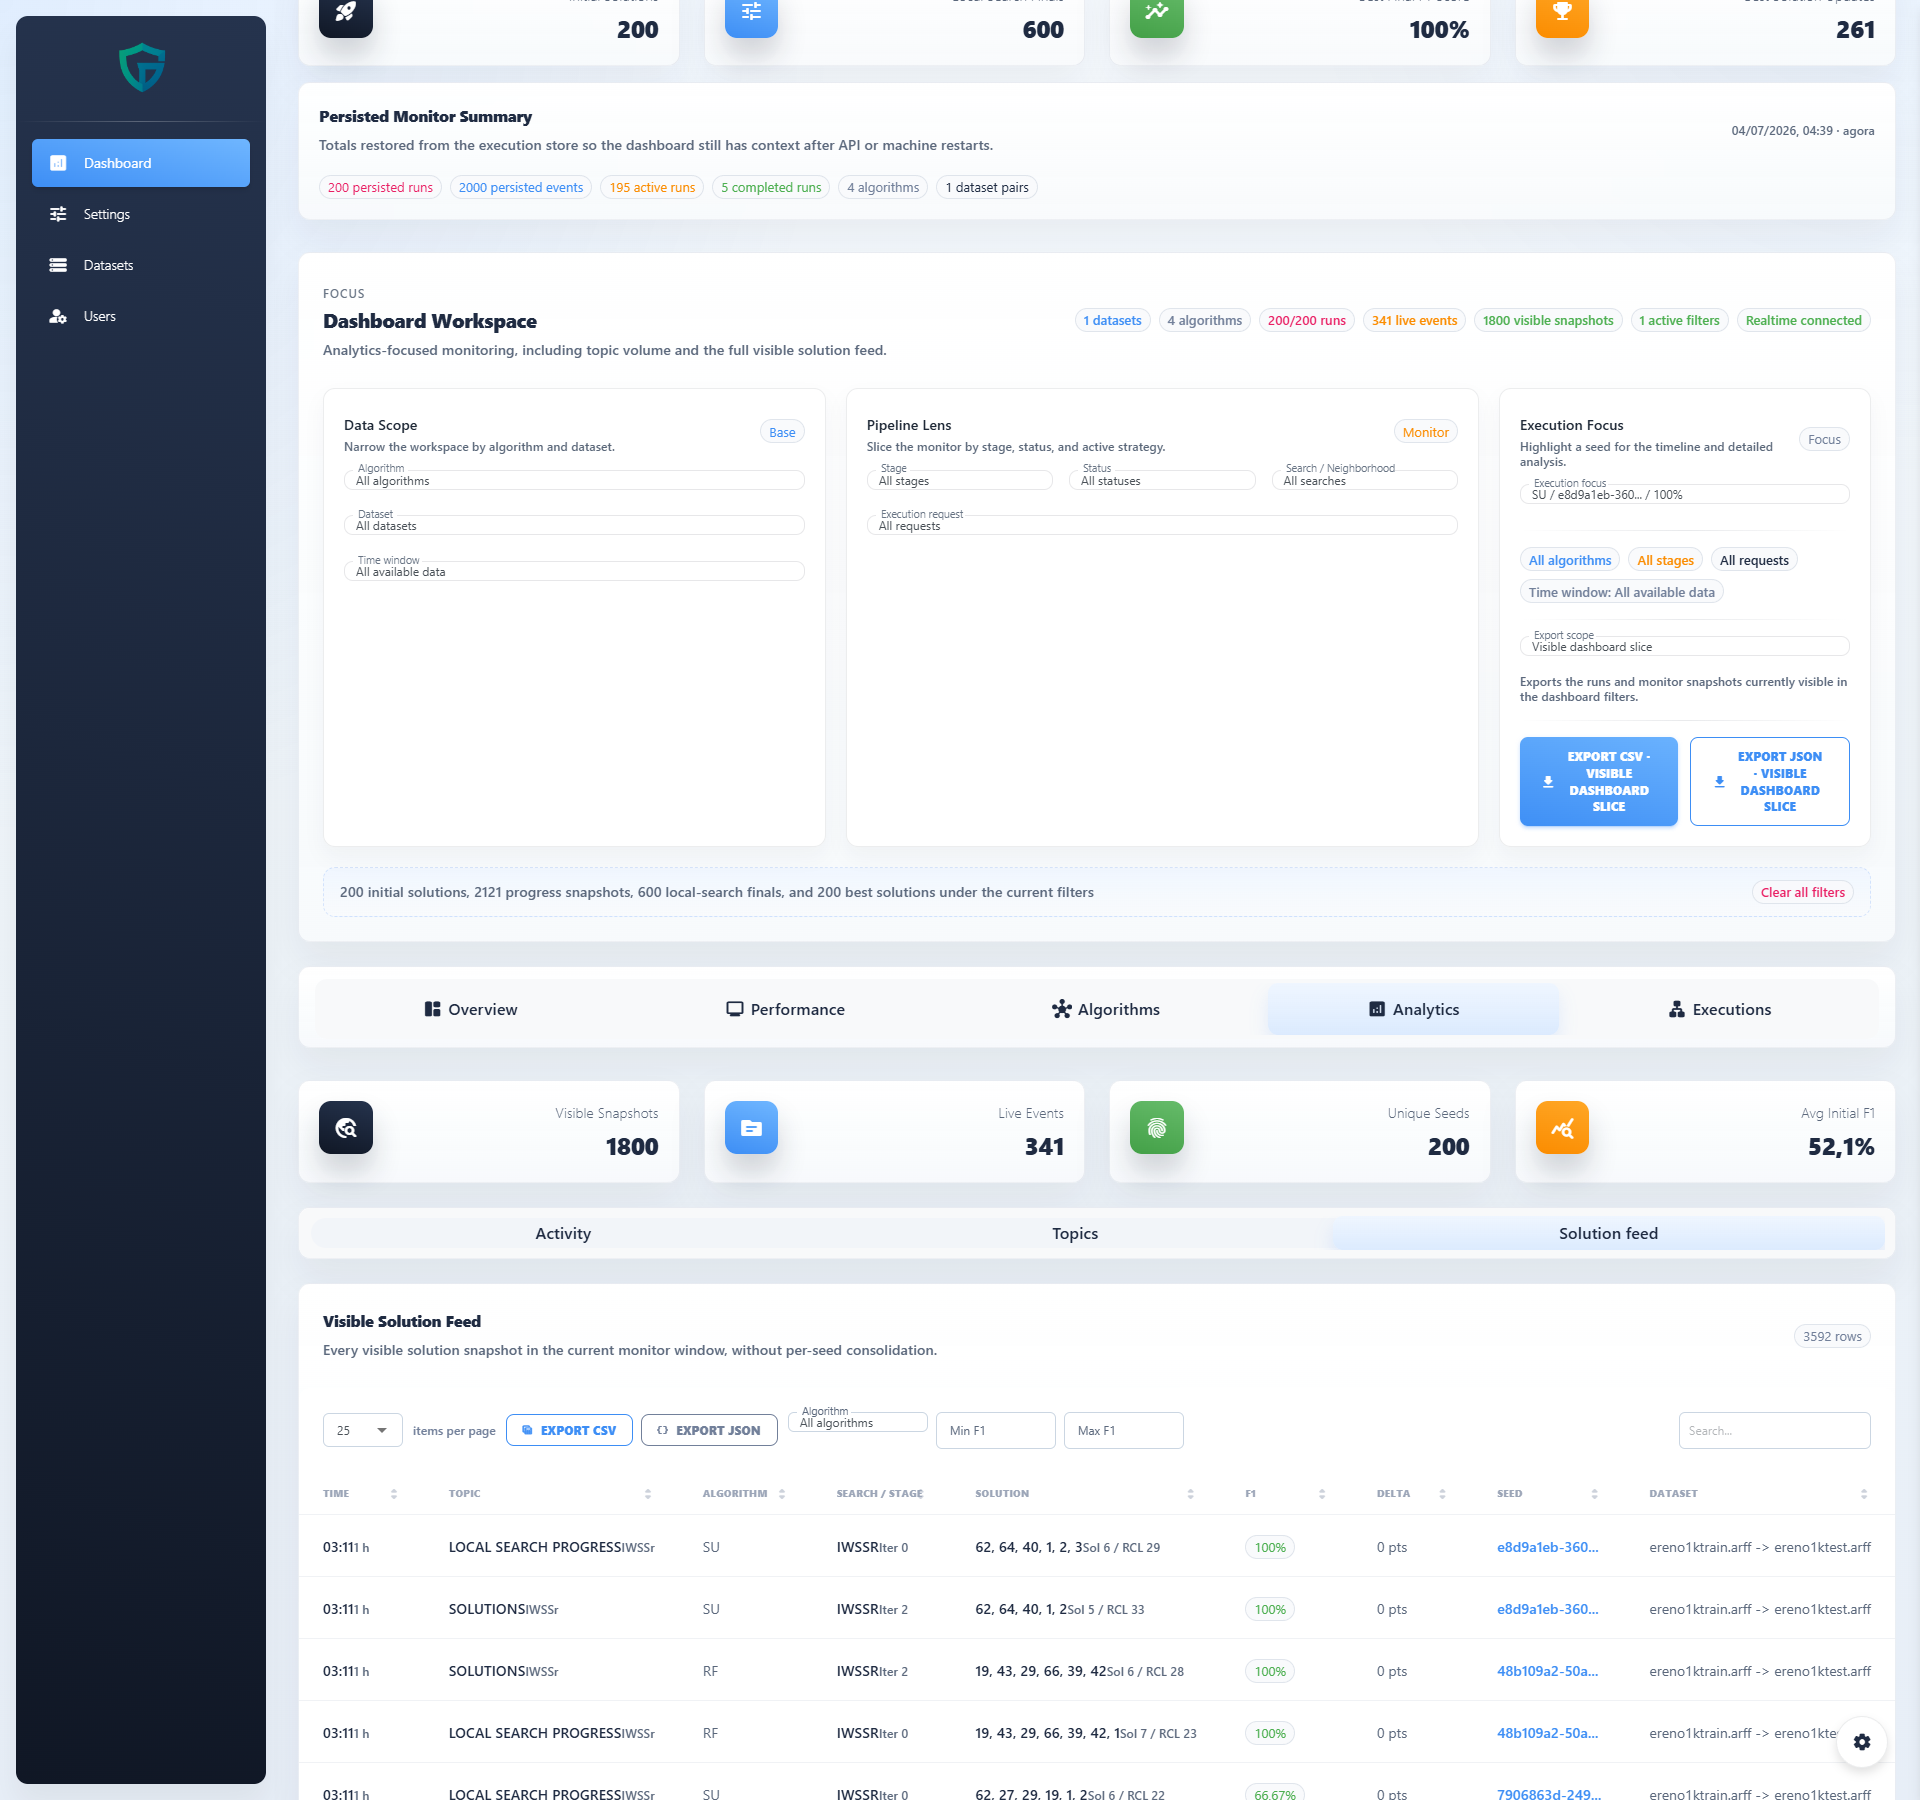
\includegraphics[width=\linewidth,height=0.80\textheight,keepaspectratio]{fig/front/07-dashboard-analytics-feed.png}
  \caption{Feed analítico persistido.}
  \label{fig:app-front-analytics-feed}
\end{figure}

\clearpage
\section{Comparação de Execuções}

Esta parte evidencia a comparação entre \textit{runs} e a inspeção de sementes selecionadas, reforçando a natureza explorável e auditável da plataforma.
As Figuras~\ref{fig:app-front-executions-comparison},~\ref{fig:app-front-executions-comparison-selected} e~\ref{fig:app-front-run-details} mostram como essa comparação é feita na prática.

\begin{figure}[!htb]
  \centering
  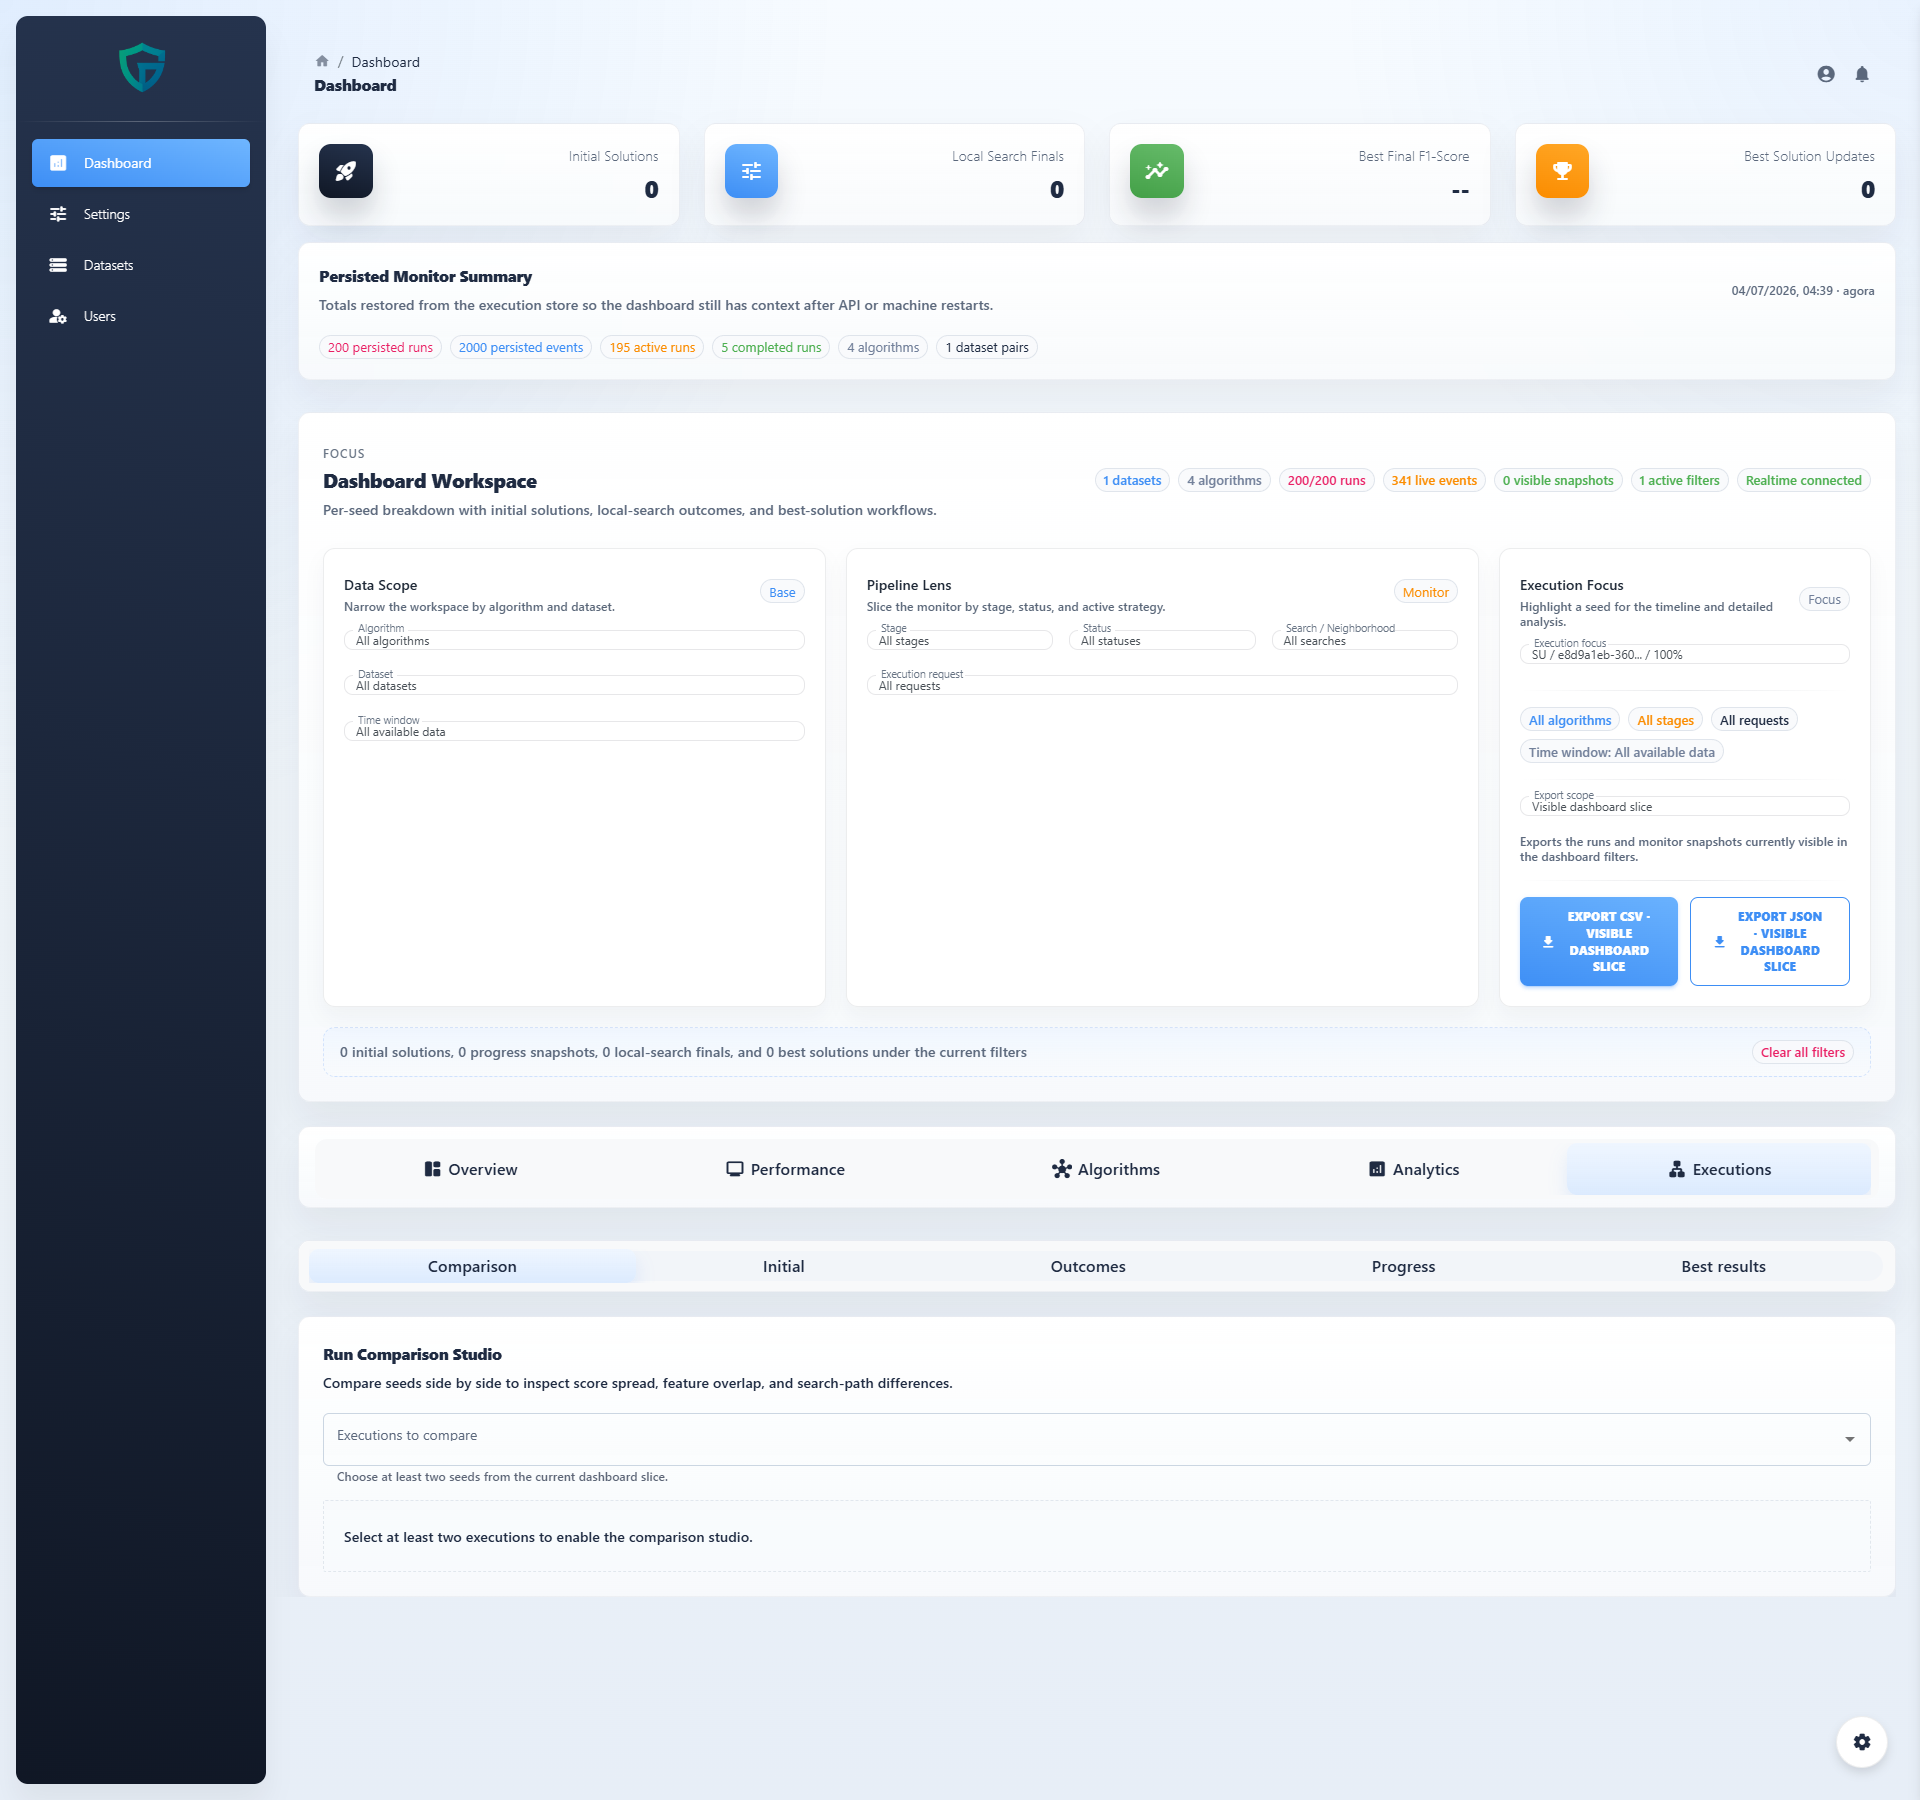
\includegraphics[width=\linewidth,height=0.80\textheight,keepaspectratio]{fig/front/08-dashboard-executions-comparison.png}
  \caption{Tela de comparação de execuções.}
  \label{fig:app-front-executions-comparison}
\end{figure}

\begin{figure}[!htb]
  \centering
  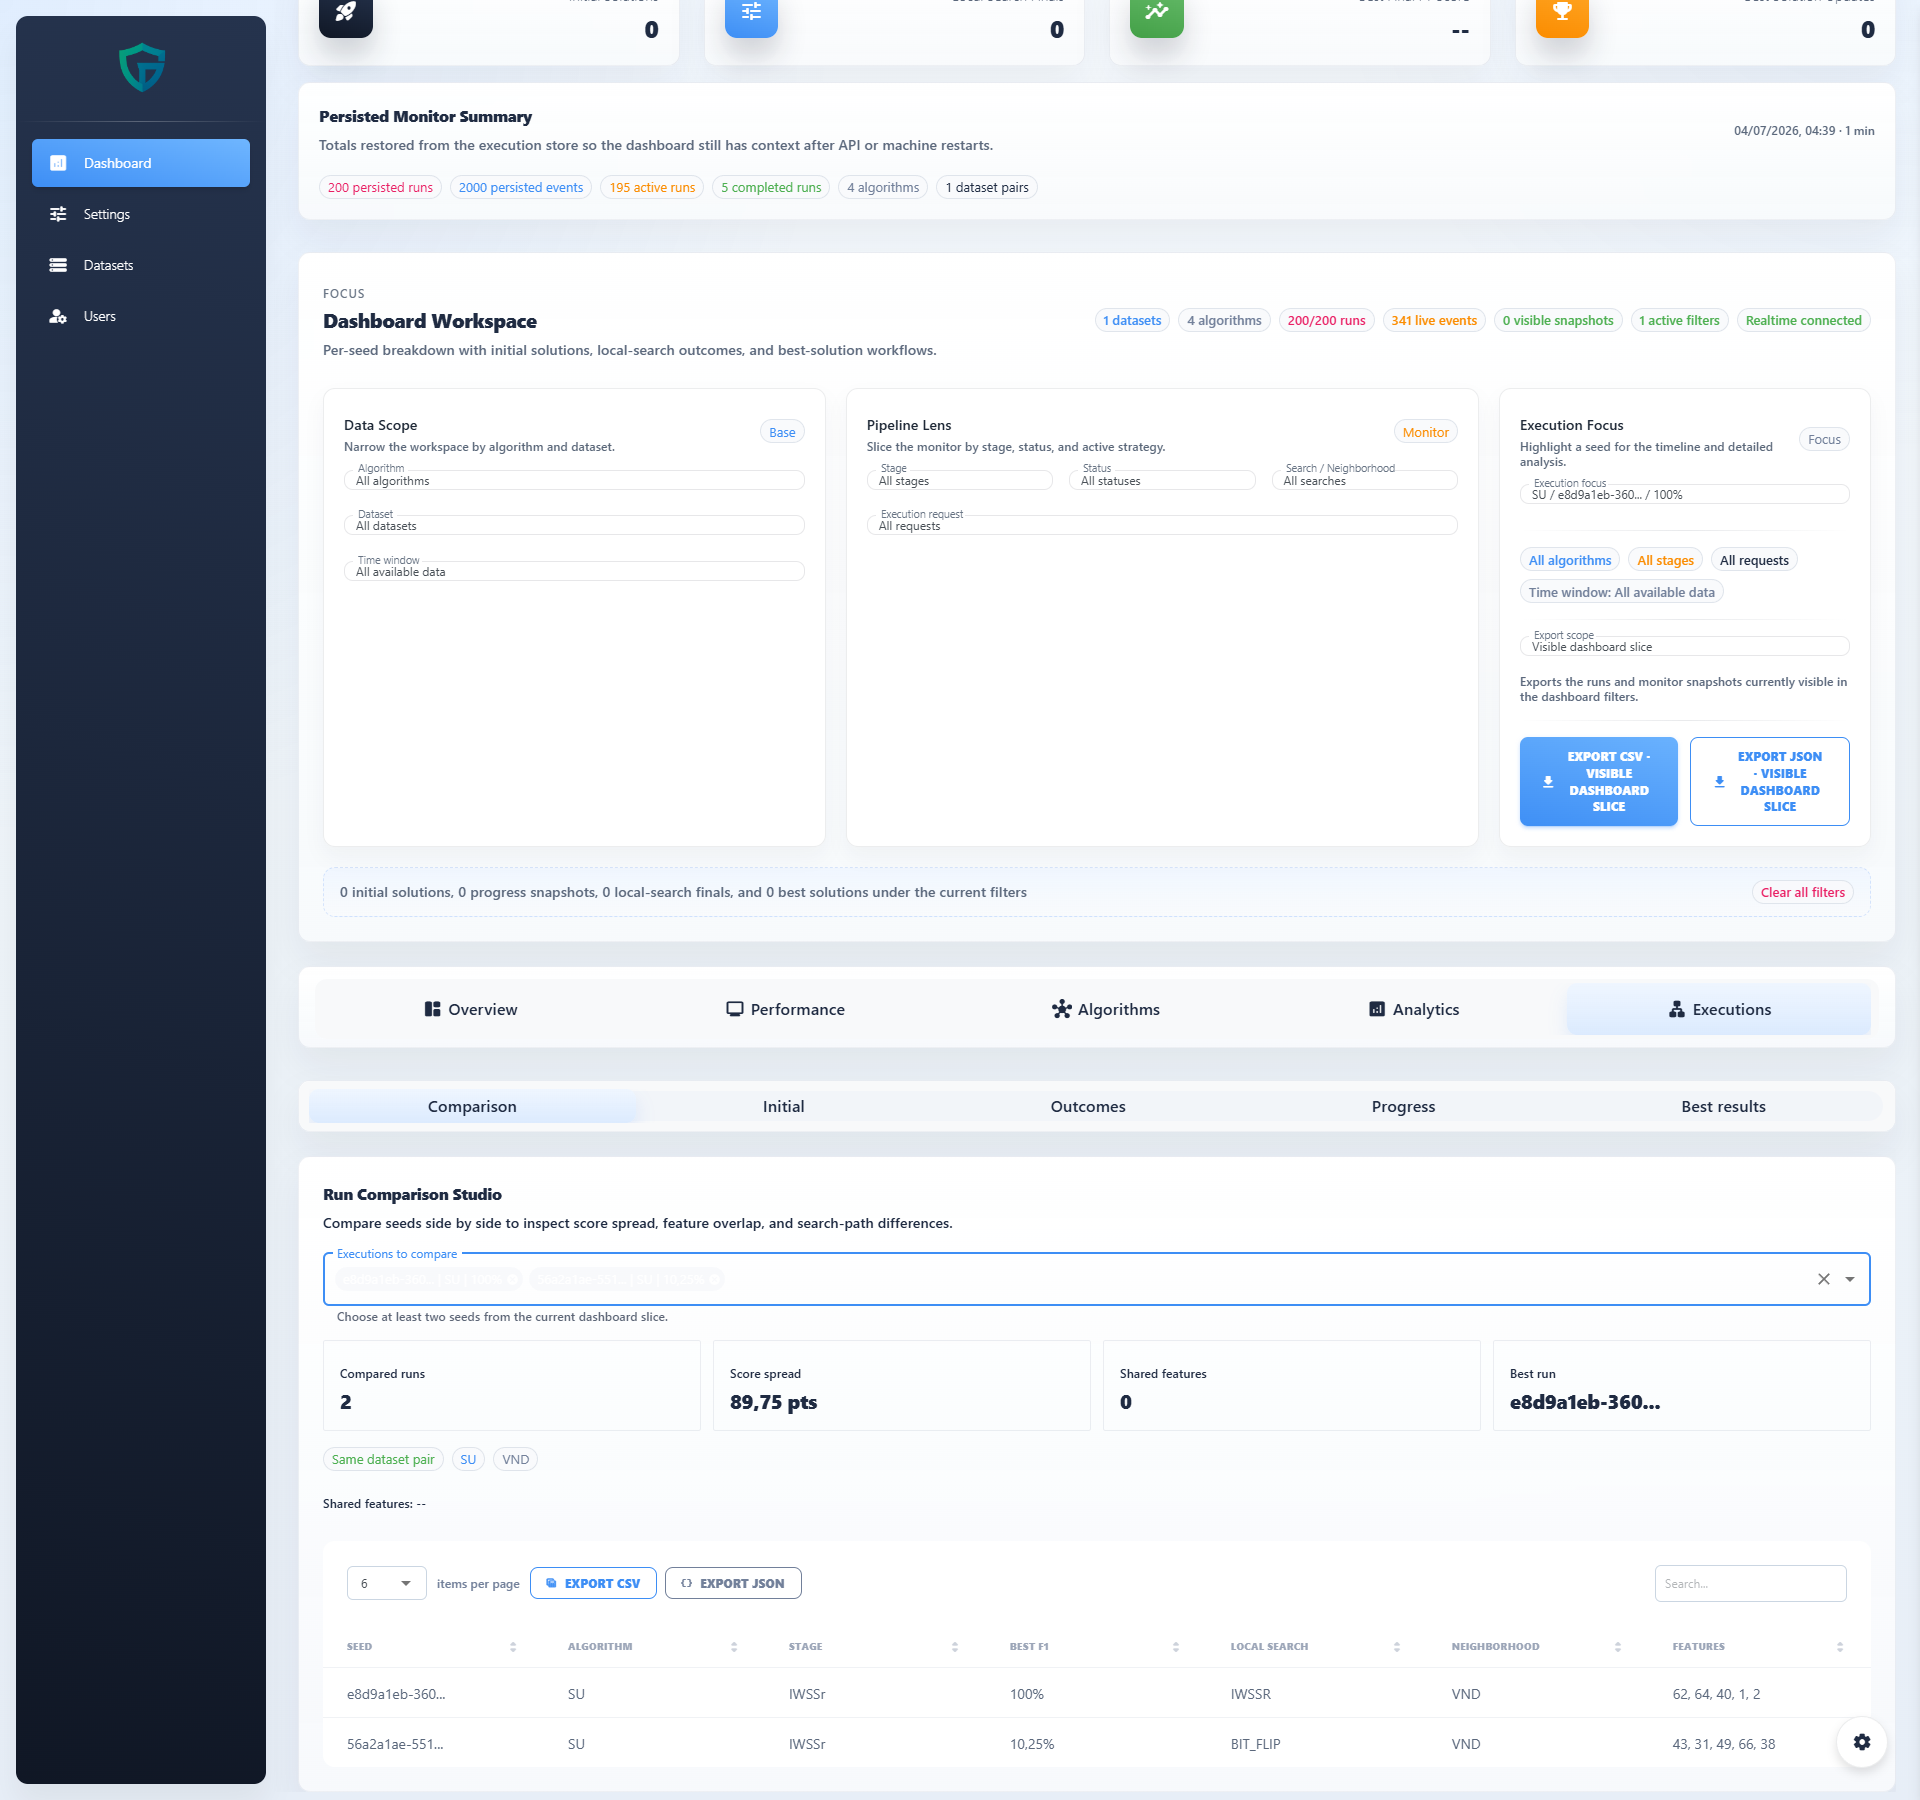
\includegraphics[width=\linewidth,height=0.80\textheight,keepaspectratio]{fig/front/13-dashboard-executions-comparison-selected.png}
  \caption{Comparação com sementes selecionadas.}
  \label{fig:app-front-executions-comparison-selected}
\end{figure}

\begin{figure}[!htb]
  \centering
  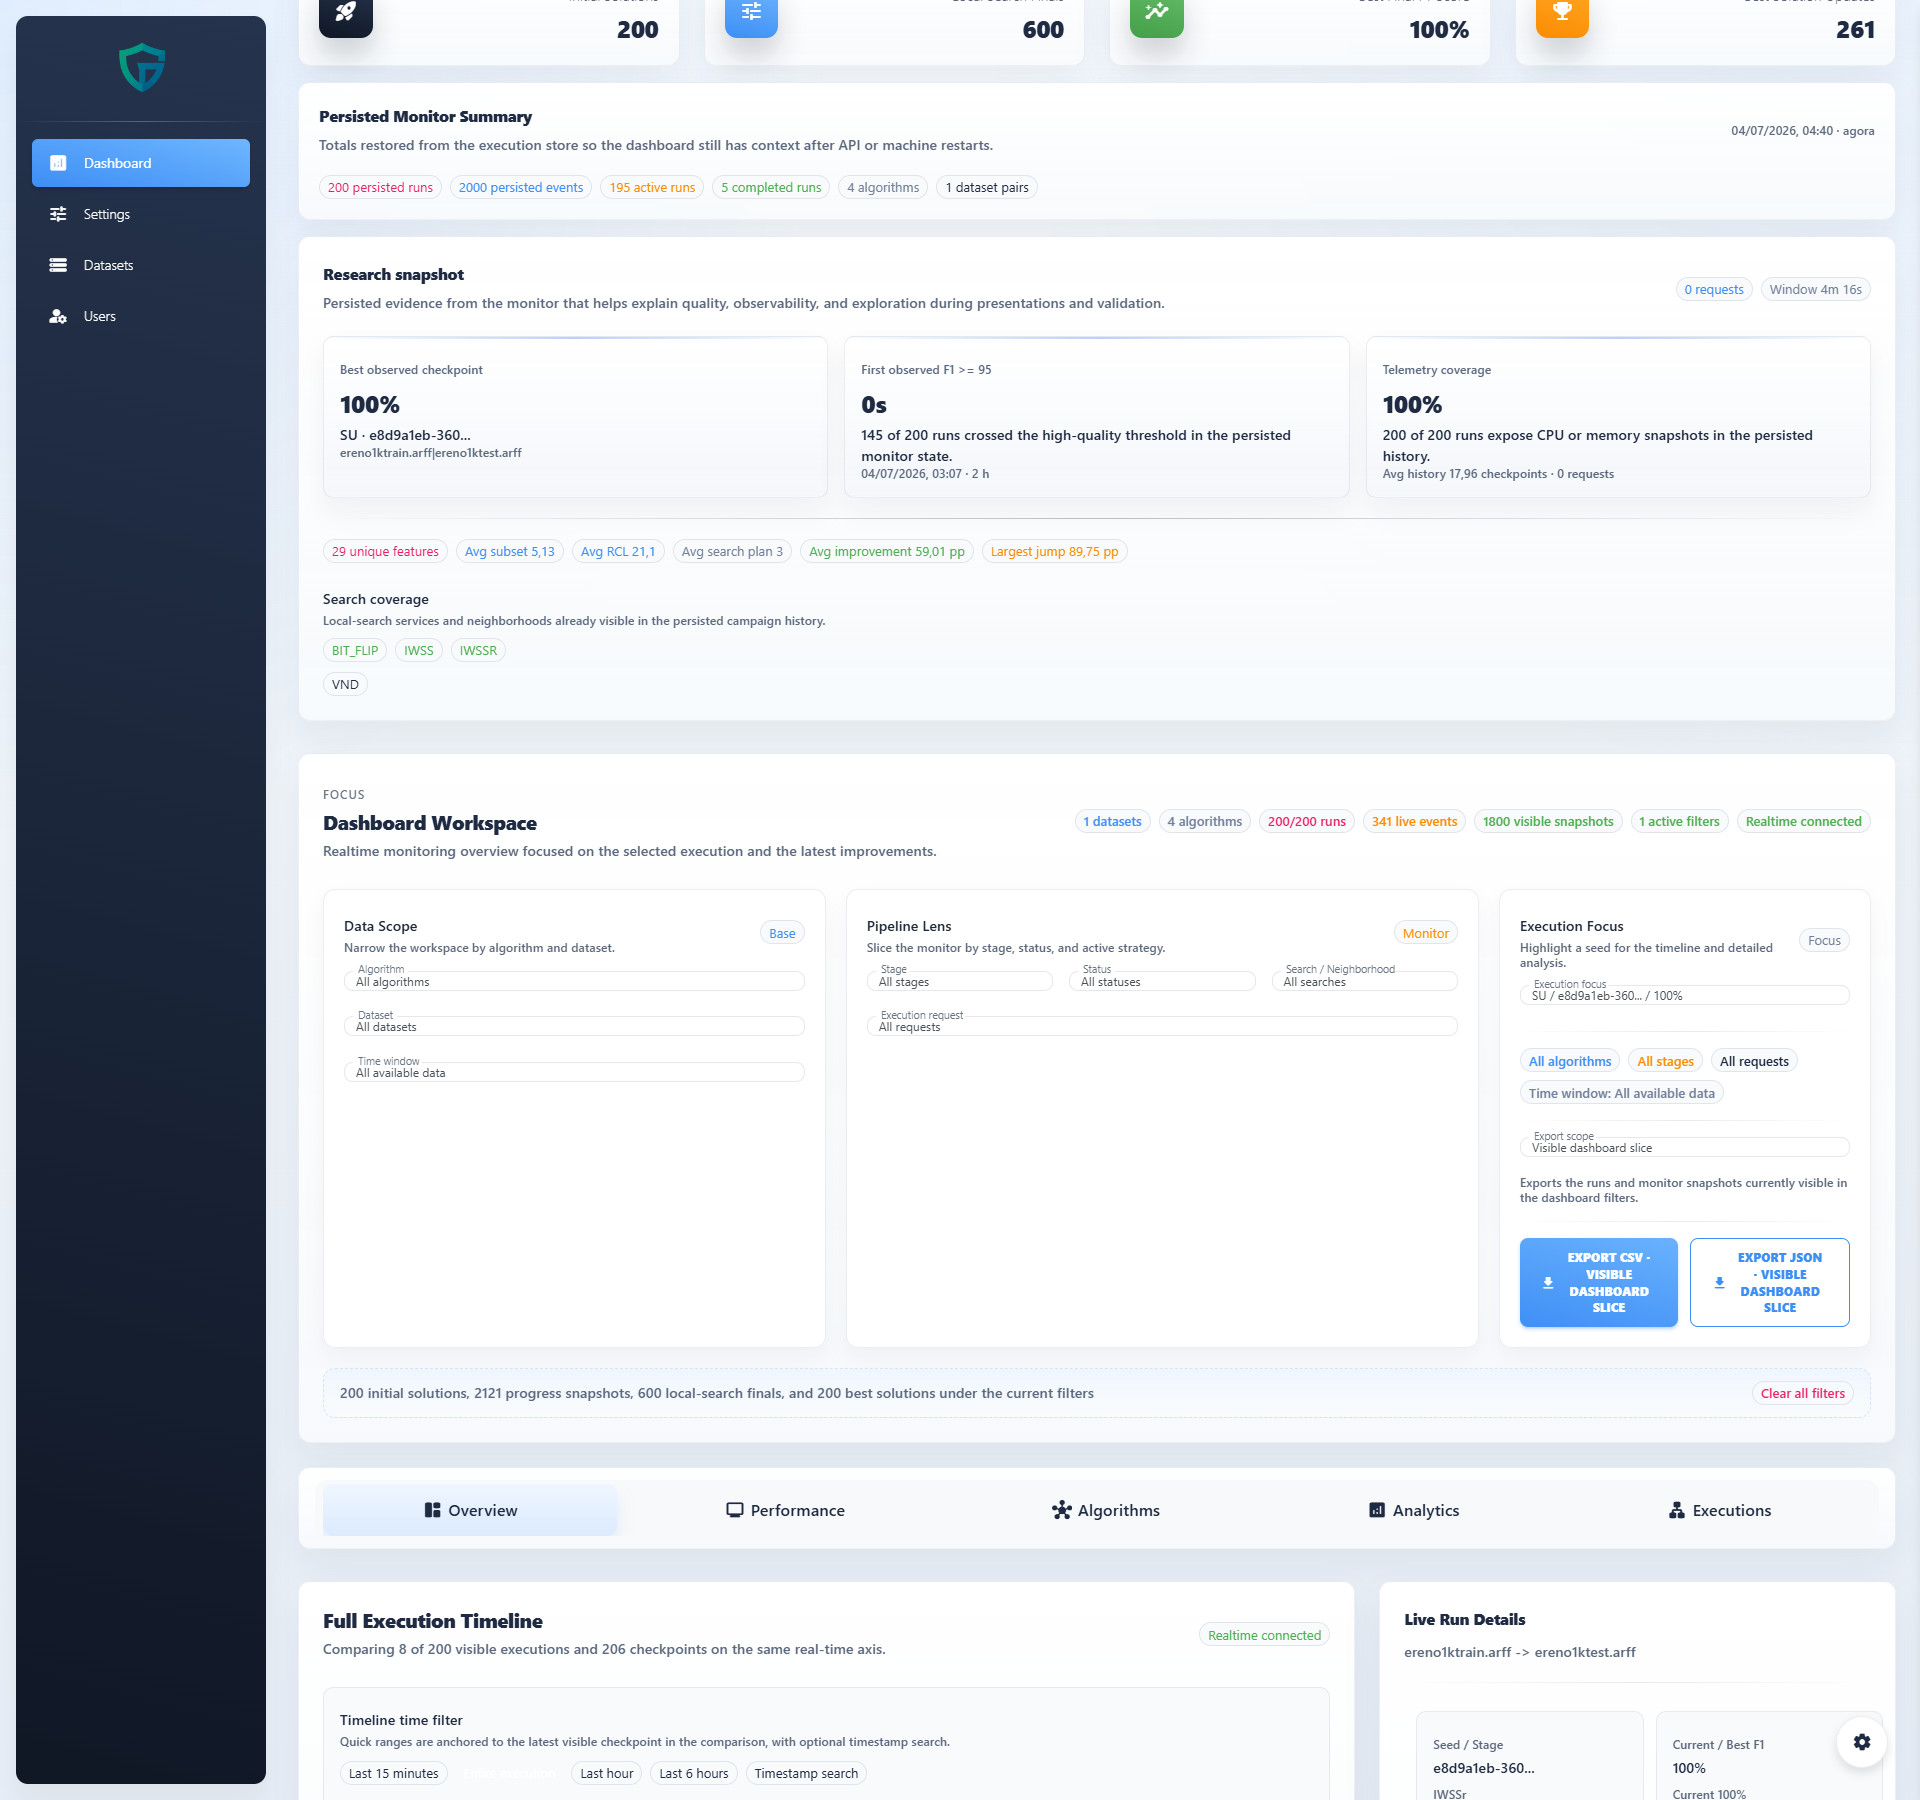
\includegraphics[width=\linewidth,height=0.80\textheight,keepaspectratio]{fig/front/14-dashboard-run-details.png}
  \caption{Detalhe de uma execução específica.}
  \label{fig:app-front-run-details}
\end{figure}

\clearpage
\section{Linha do Tempo e Resultados}

As capturas desta seção mostram como o front exibe a evolução das soluções ao longo do tempo, apoiando a leitura do progresso e da qualidade das execuções.
As Figuras~\ref{fig:app-front-executions-initial},~\ref{fig:app-front-executions-outcomes},~\ref{fig:app-front-executions-progress} e~\ref{fig:app-front-executions-best} completam esse ciclo visual.

\begin{figure}[!htb]
  \centering
  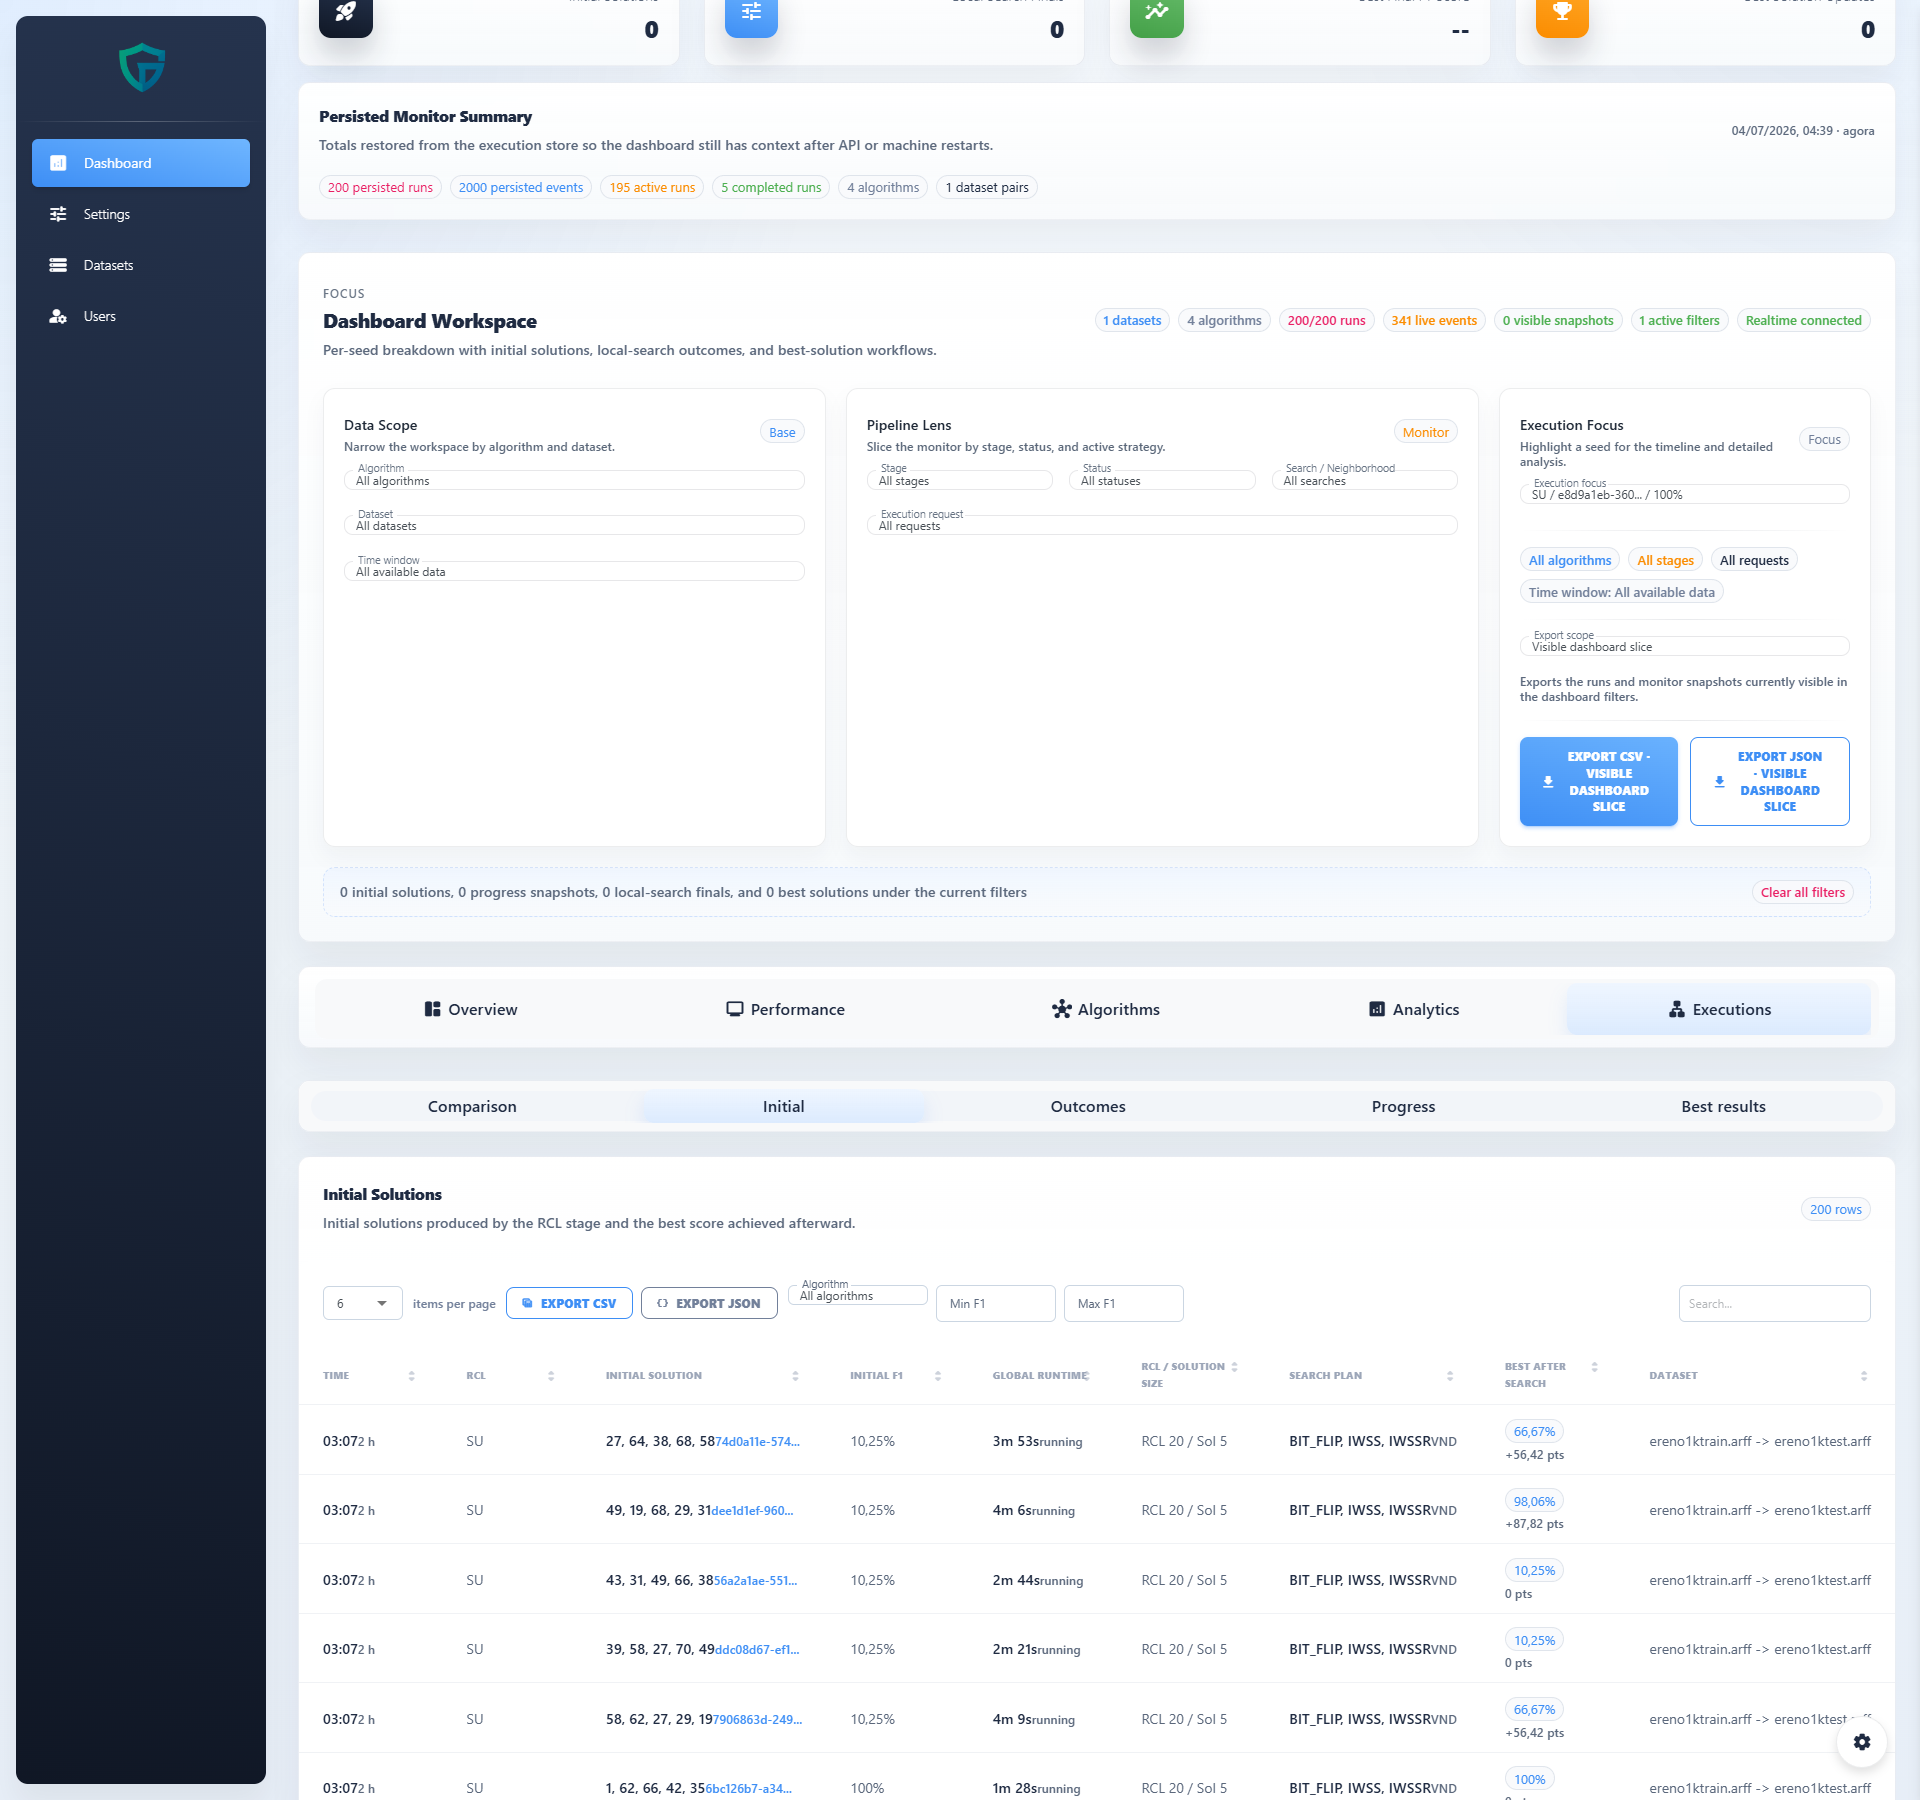
\includegraphics[width=\linewidth,height=0.80\textheight,keepaspectratio]{fig/front/09-dashboard-executions-initial.png}
  \caption{Soluções iniciais.}
  \label{fig:app-front-executions-initial}
\end{figure}

\begin{figure}[!htb]
  \centering
  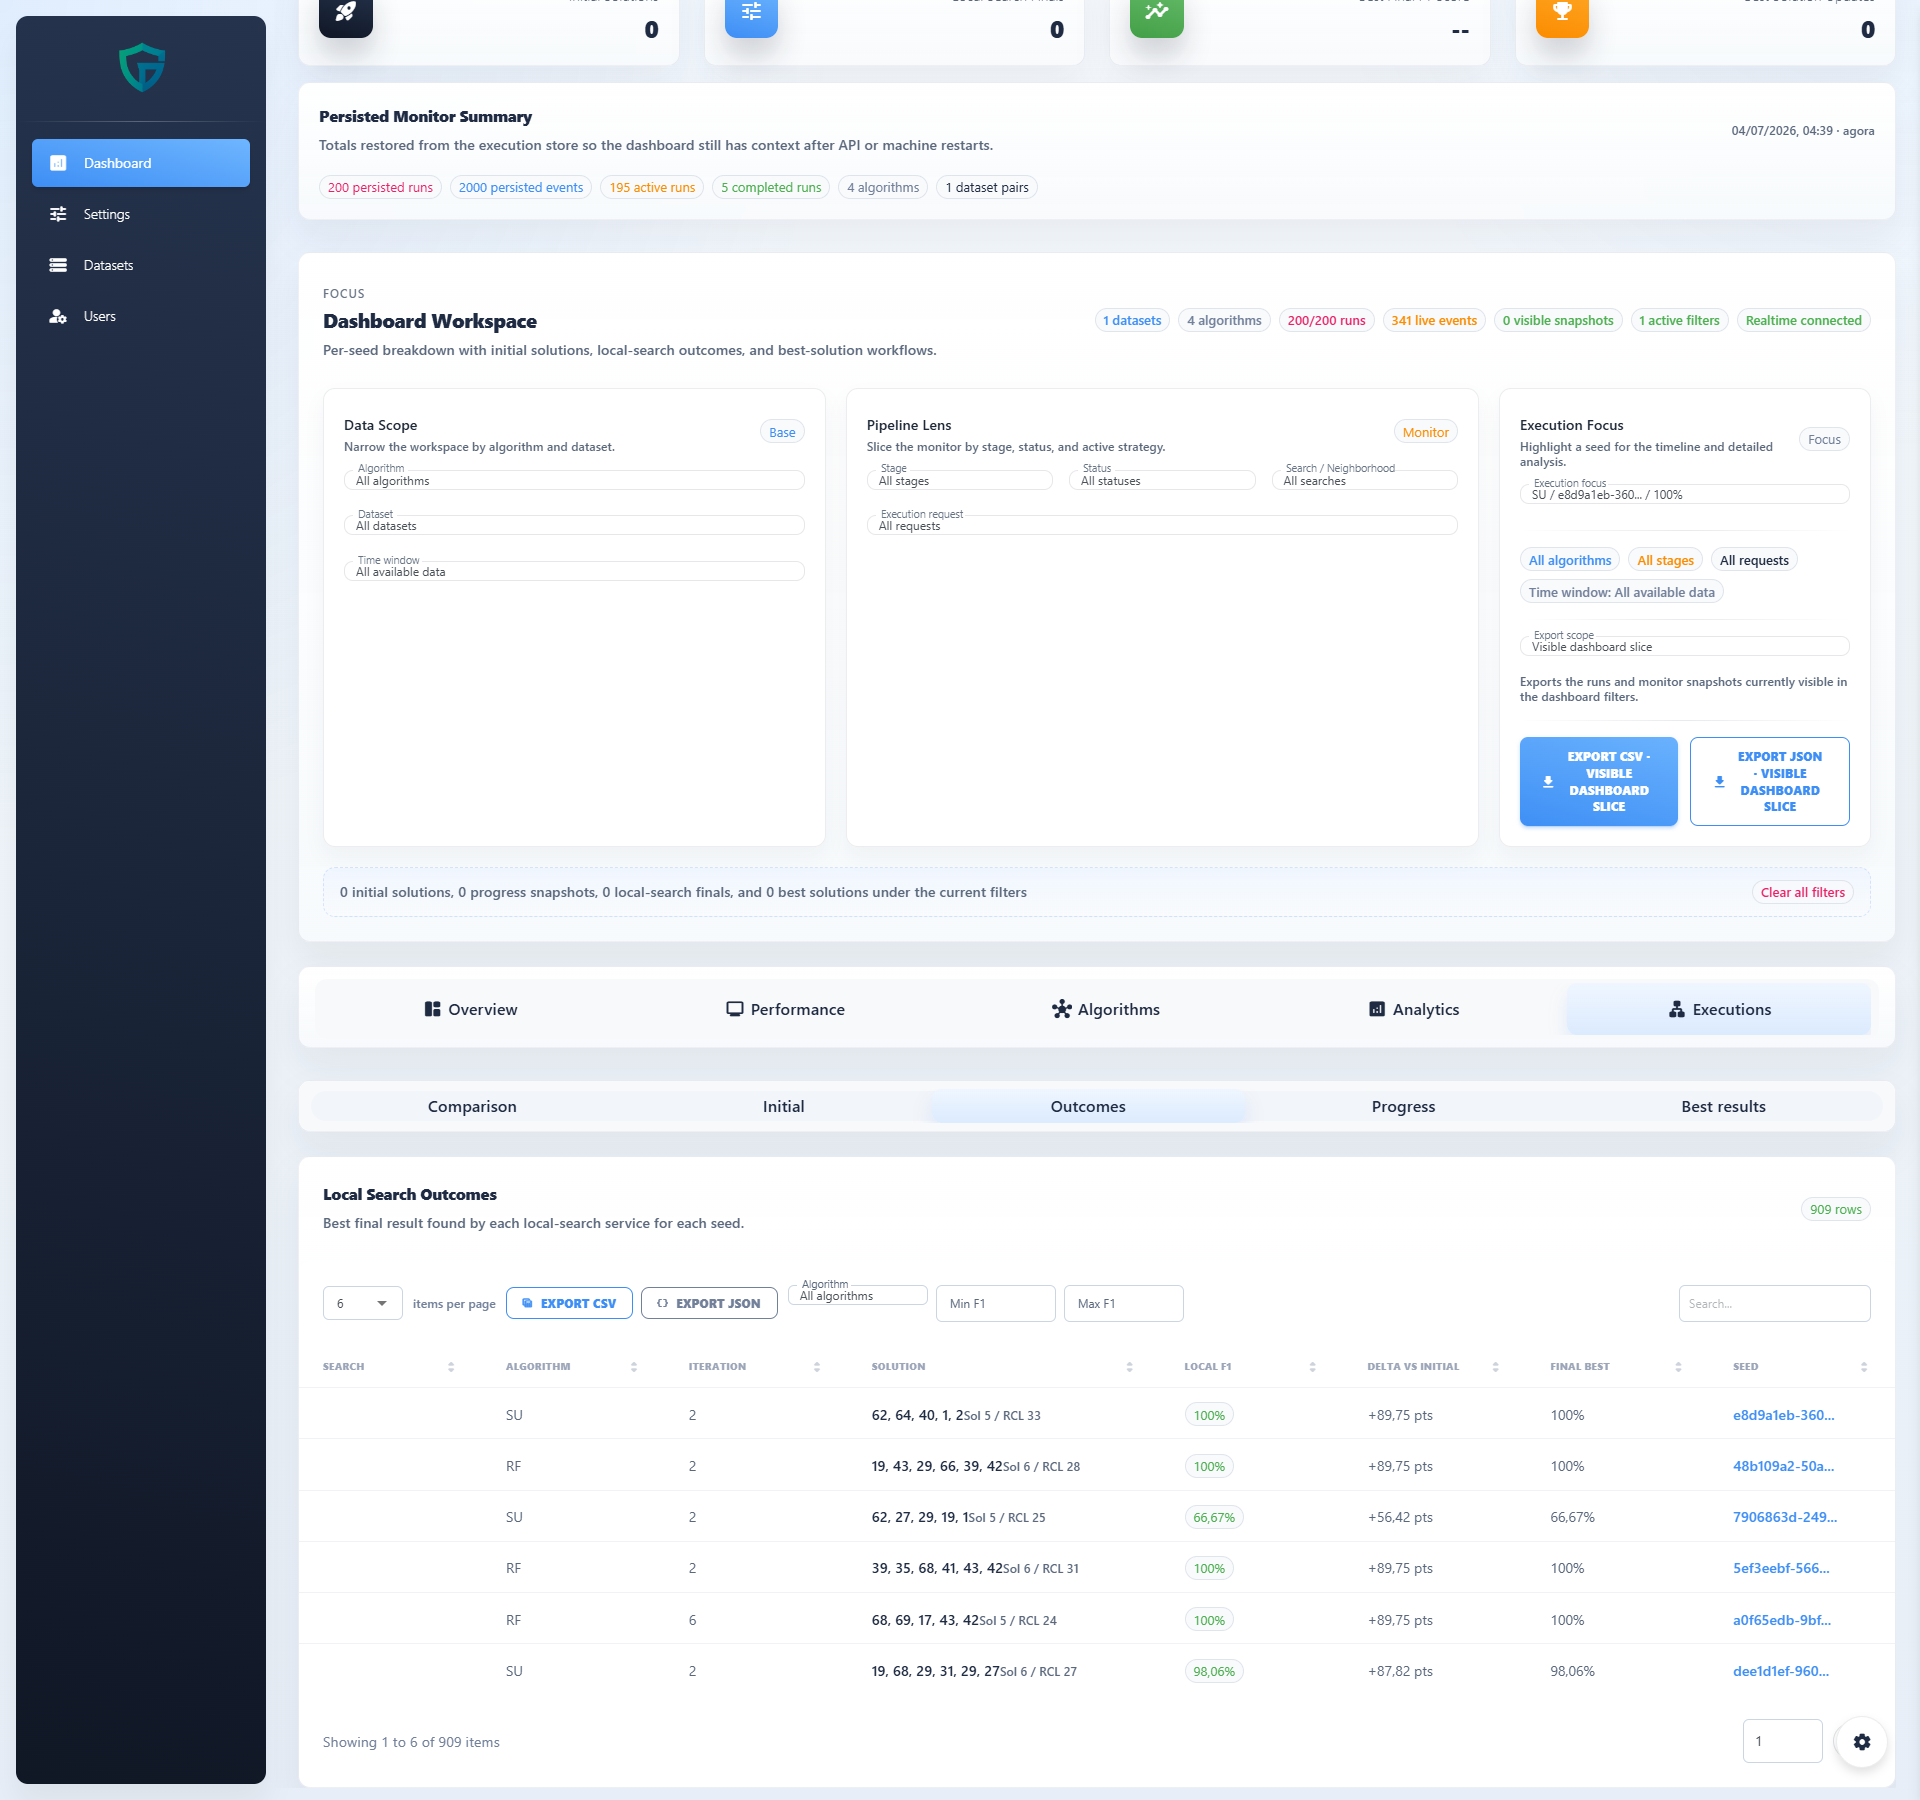
\includegraphics[width=\linewidth,height=0.80\textheight,keepaspectratio]{fig/front/10-dashboard-executions-outcomes.png}
  \caption{Resultados consolidados.}
  \label{fig:app-front-executions-outcomes}
\end{figure}

\begin{figure}[!htb]
  \centering
  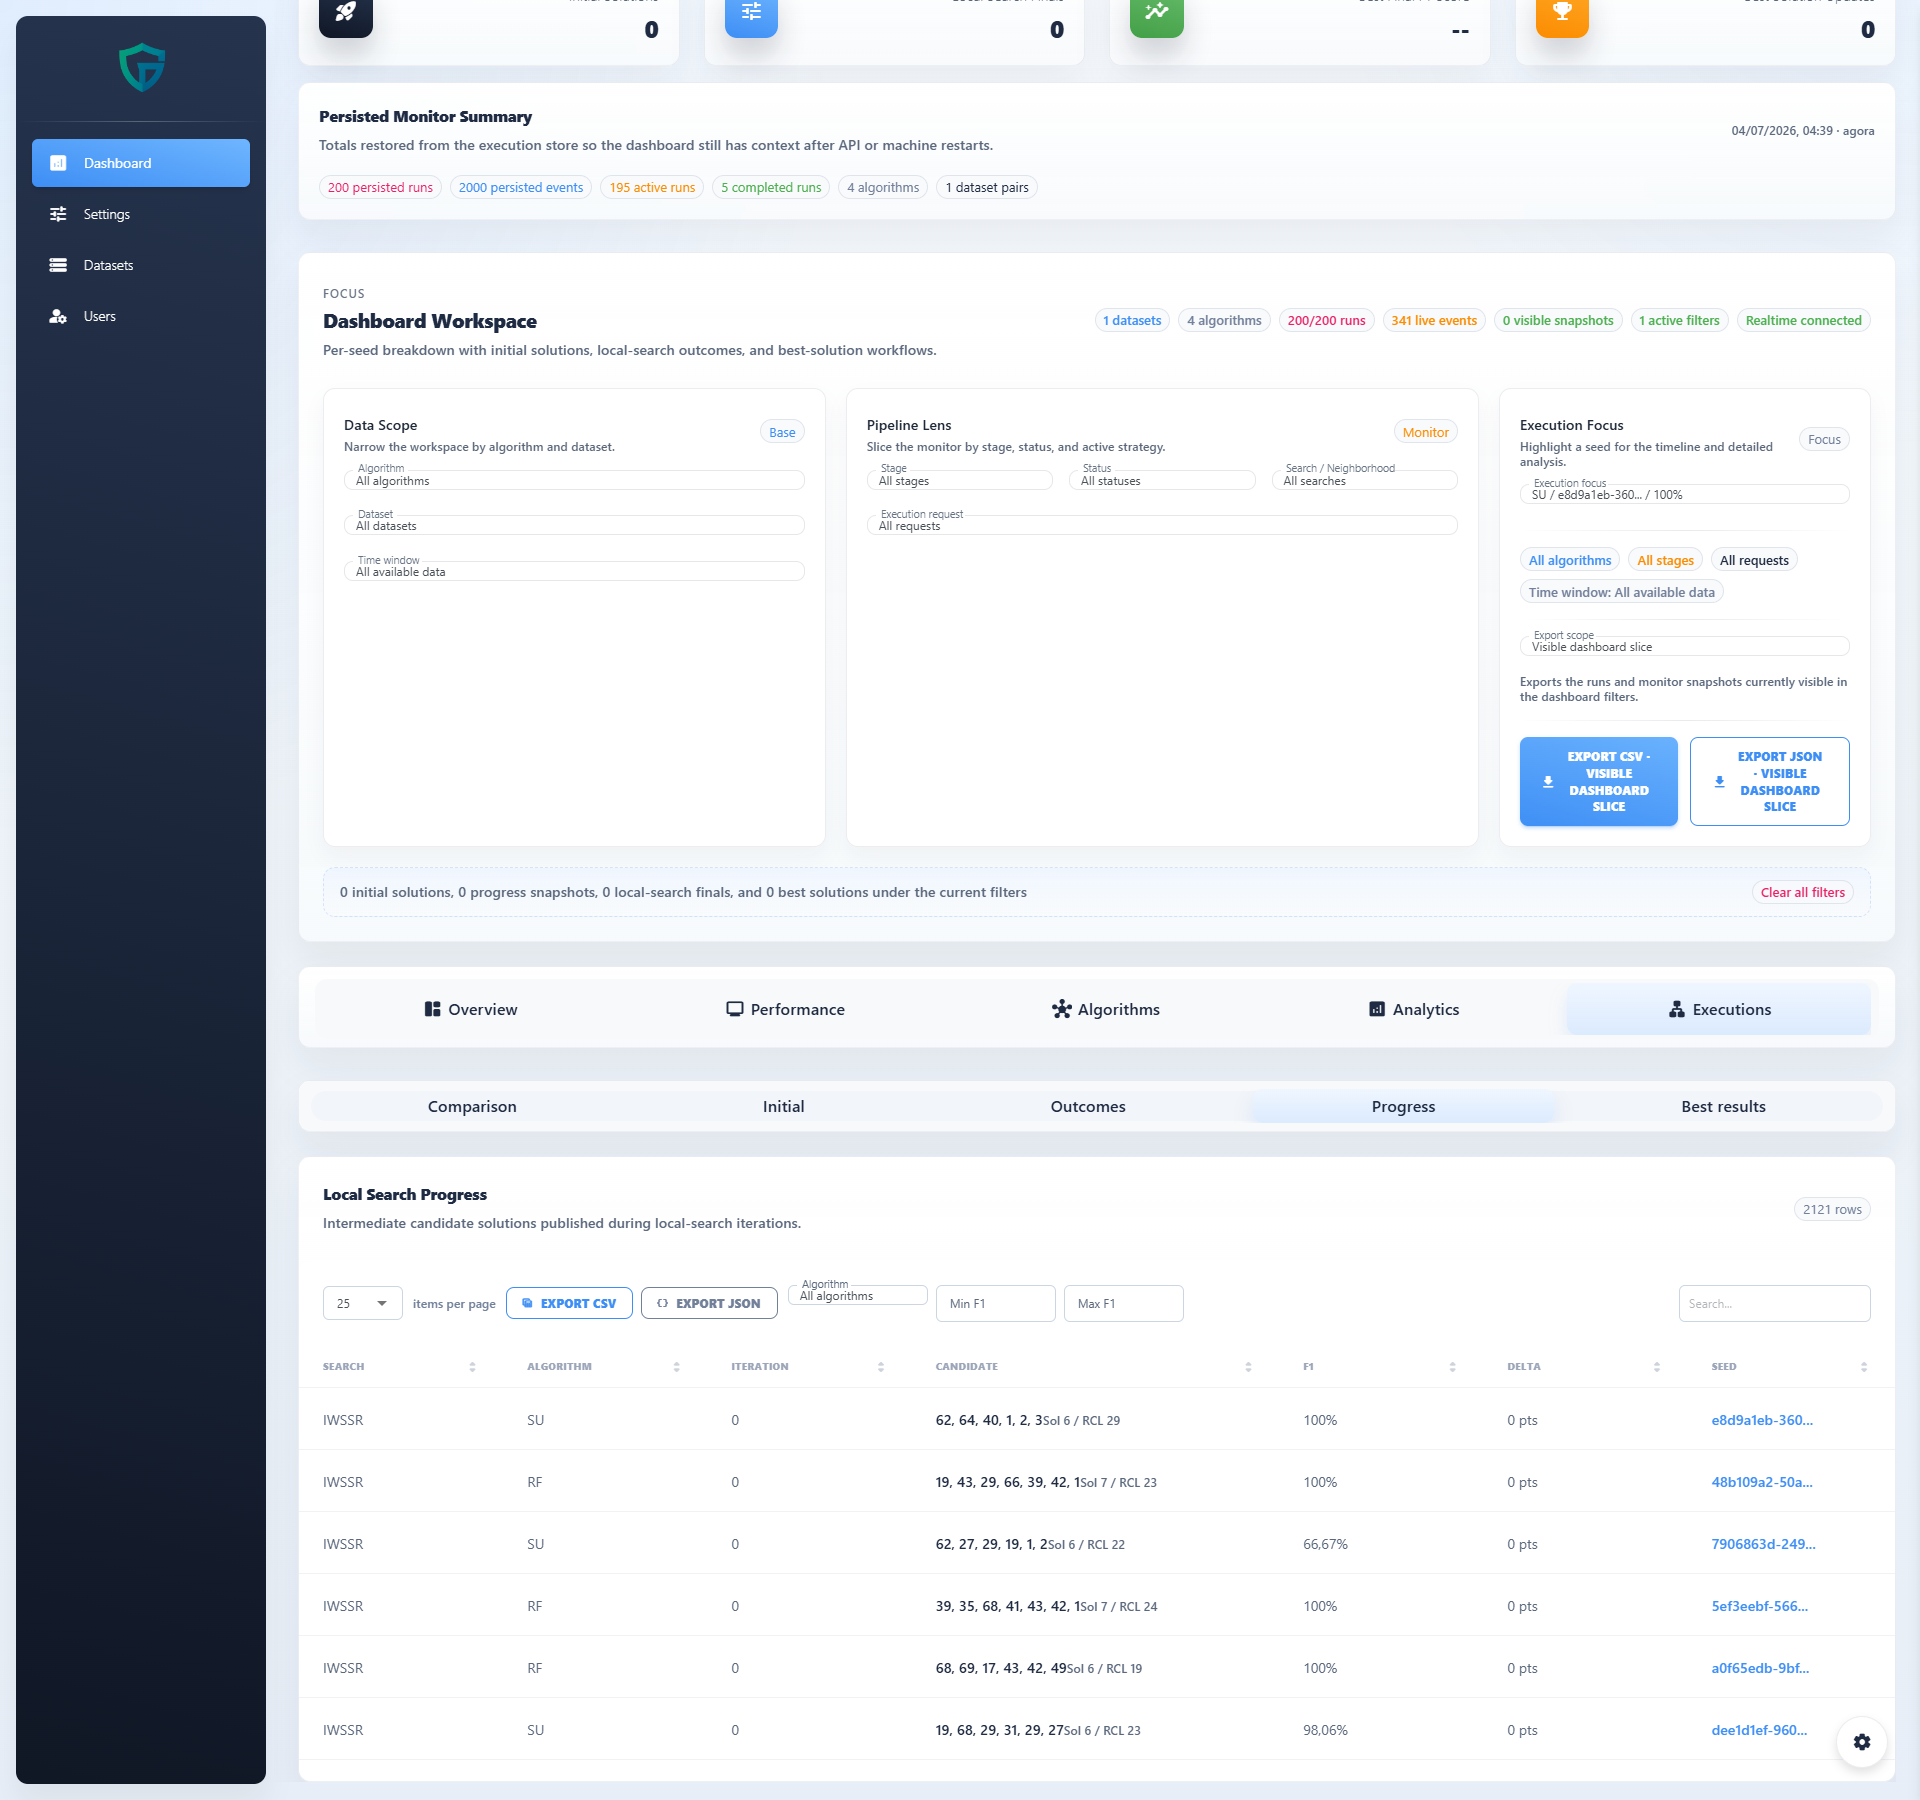
\includegraphics[width=\linewidth,height=0.80\textheight,keepaspectratio]{fig/front/11-dashboard-executions-progress.png}
  \caption{Progresso da execução.}
  \label{fig:app-front-executions-progress}
\end{figure}

\begin{figure}[!htb]
  \centering
  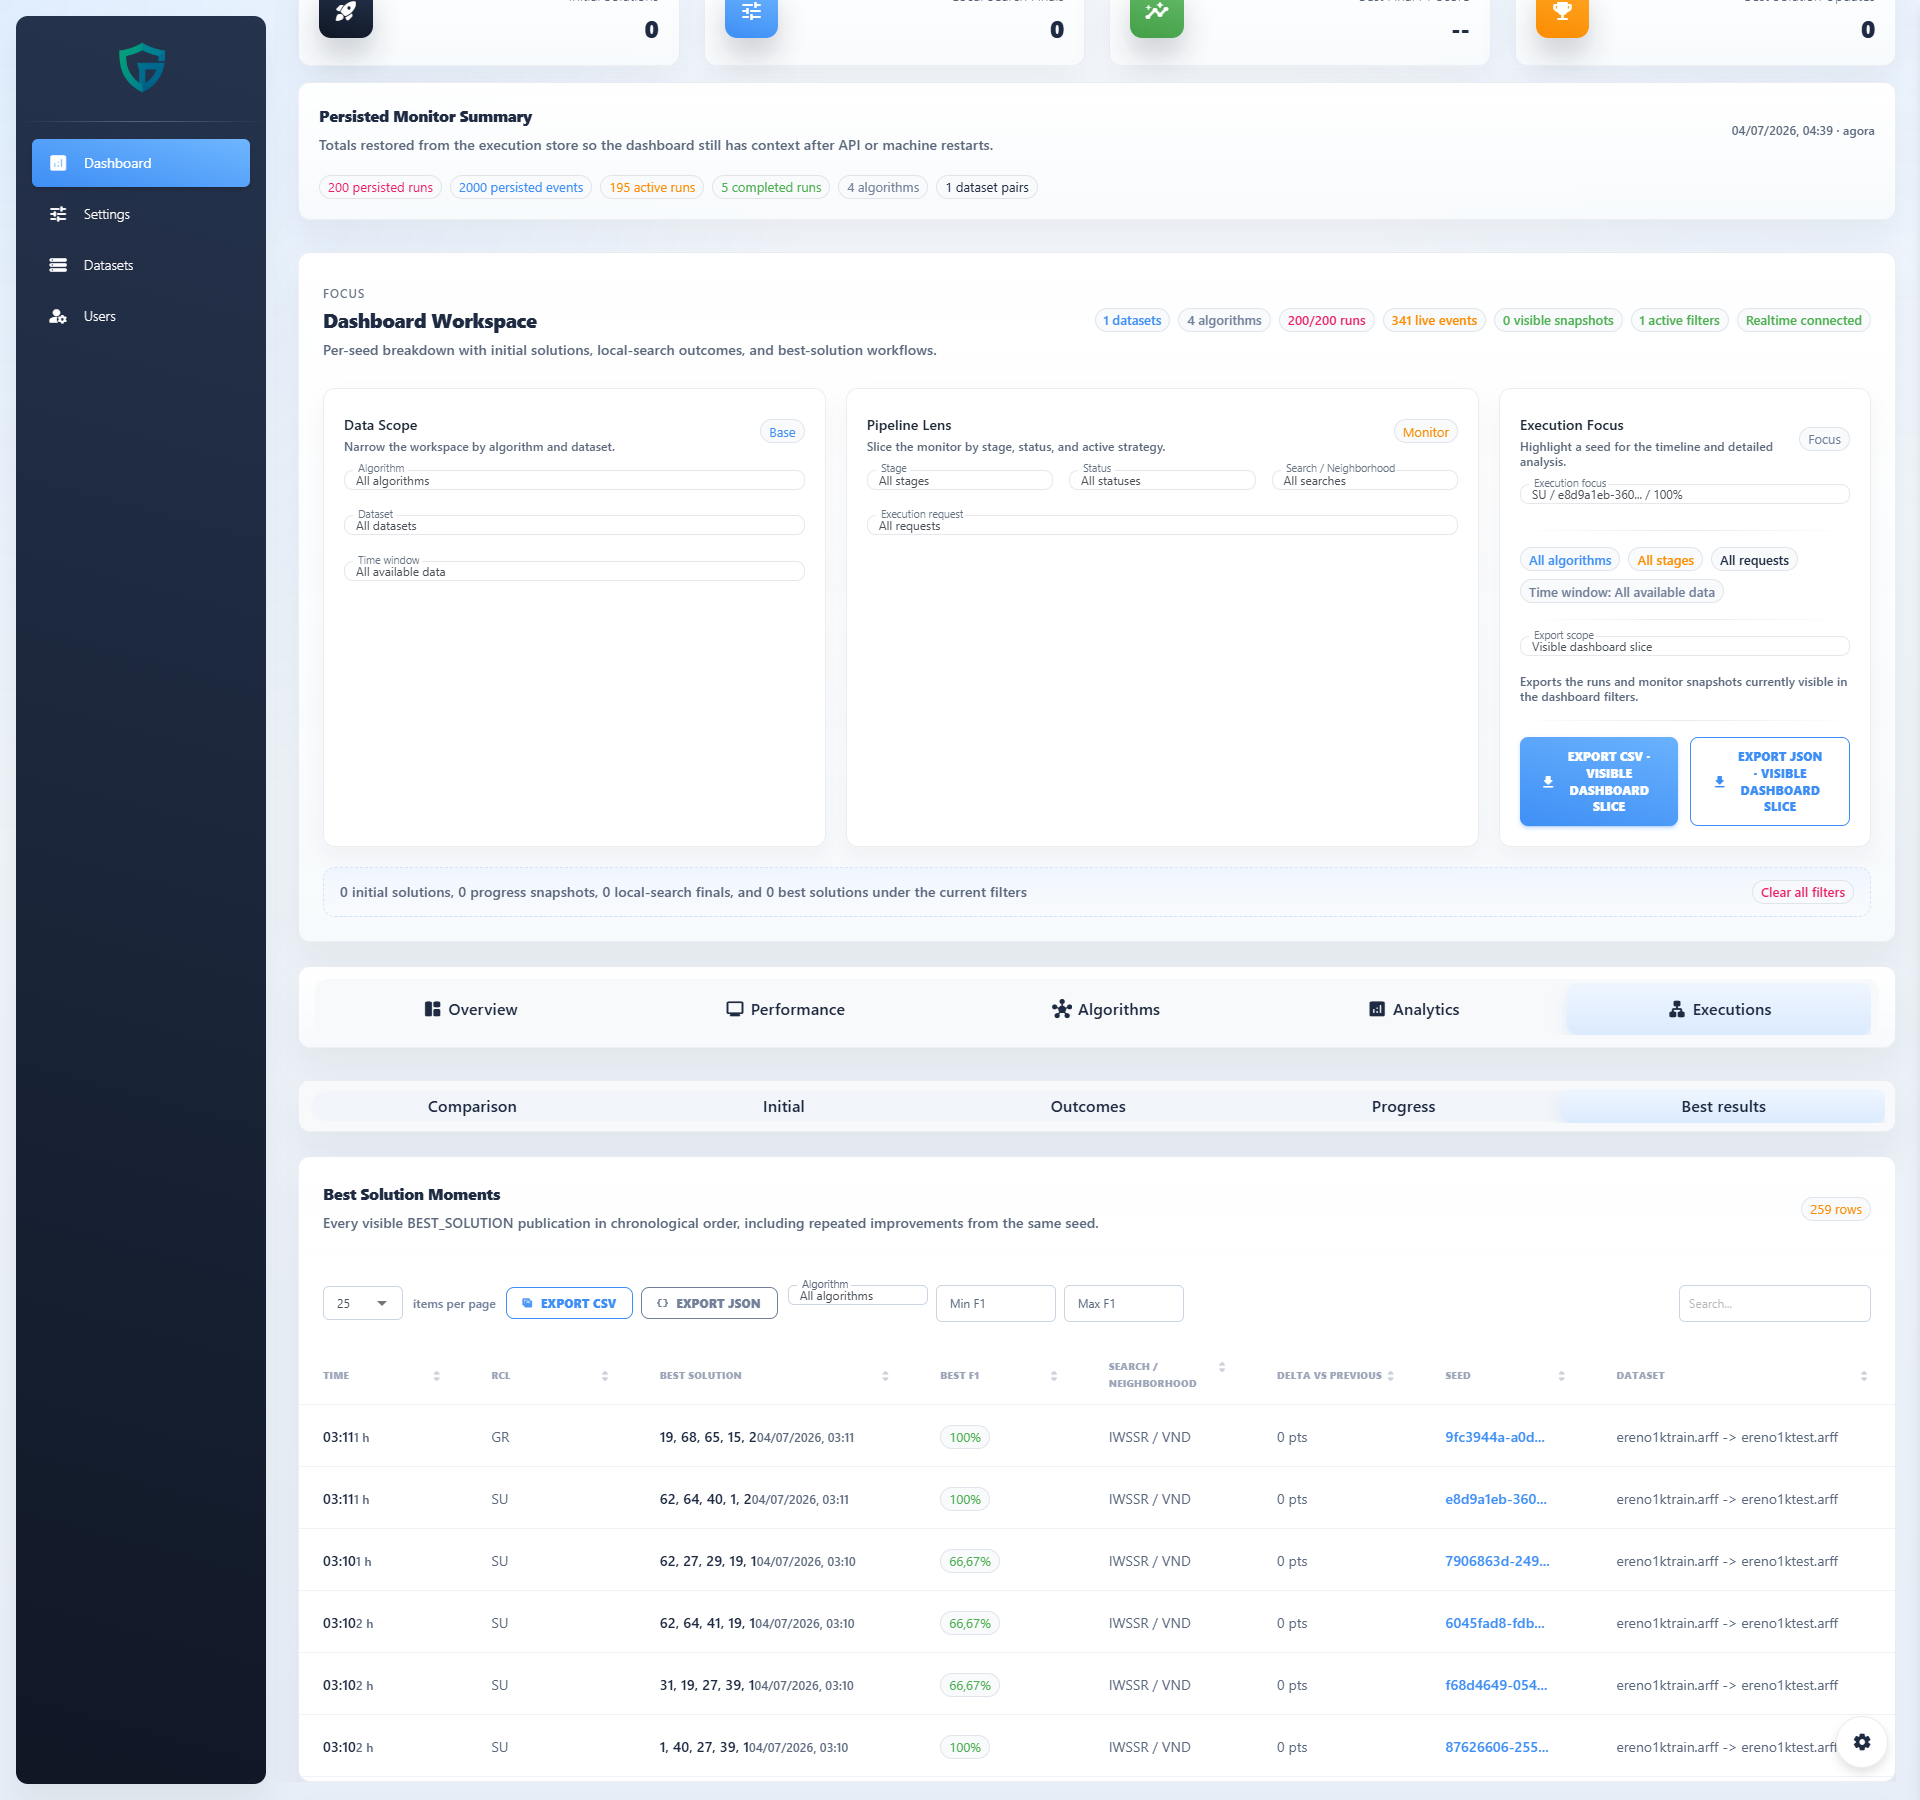
\includegraphics[width=\linewidth,height=0.80\textheight,keepaspectratio]{fig/front/12-dashboard-executions-best.png}
  \caption{Melhores soluções.}
  \label{fig:app-front-executions-best}
\end{figure}

\clearpage
\section{Configurações e Administração}

Por fim, as telas administrativas demonstram que a plataforma também cobre os aspectos de operação e manutenção, não apenas a visualização de resultados.
As Figuras~\ref{fig:app-front-settings-execution},~\ref{fig:app-front-settings-datasets},~\ref{fig:app-front-settings-operations},~\ref{fig:app-front-settings-reset},~\ref{fig:app-front-datasets},~\ref{fig:app-front-users-list} e~\ref{fig:app-front-user-edit} mostram o conjunto administrativo.

\begin{figure}[!htb]
  \centering
  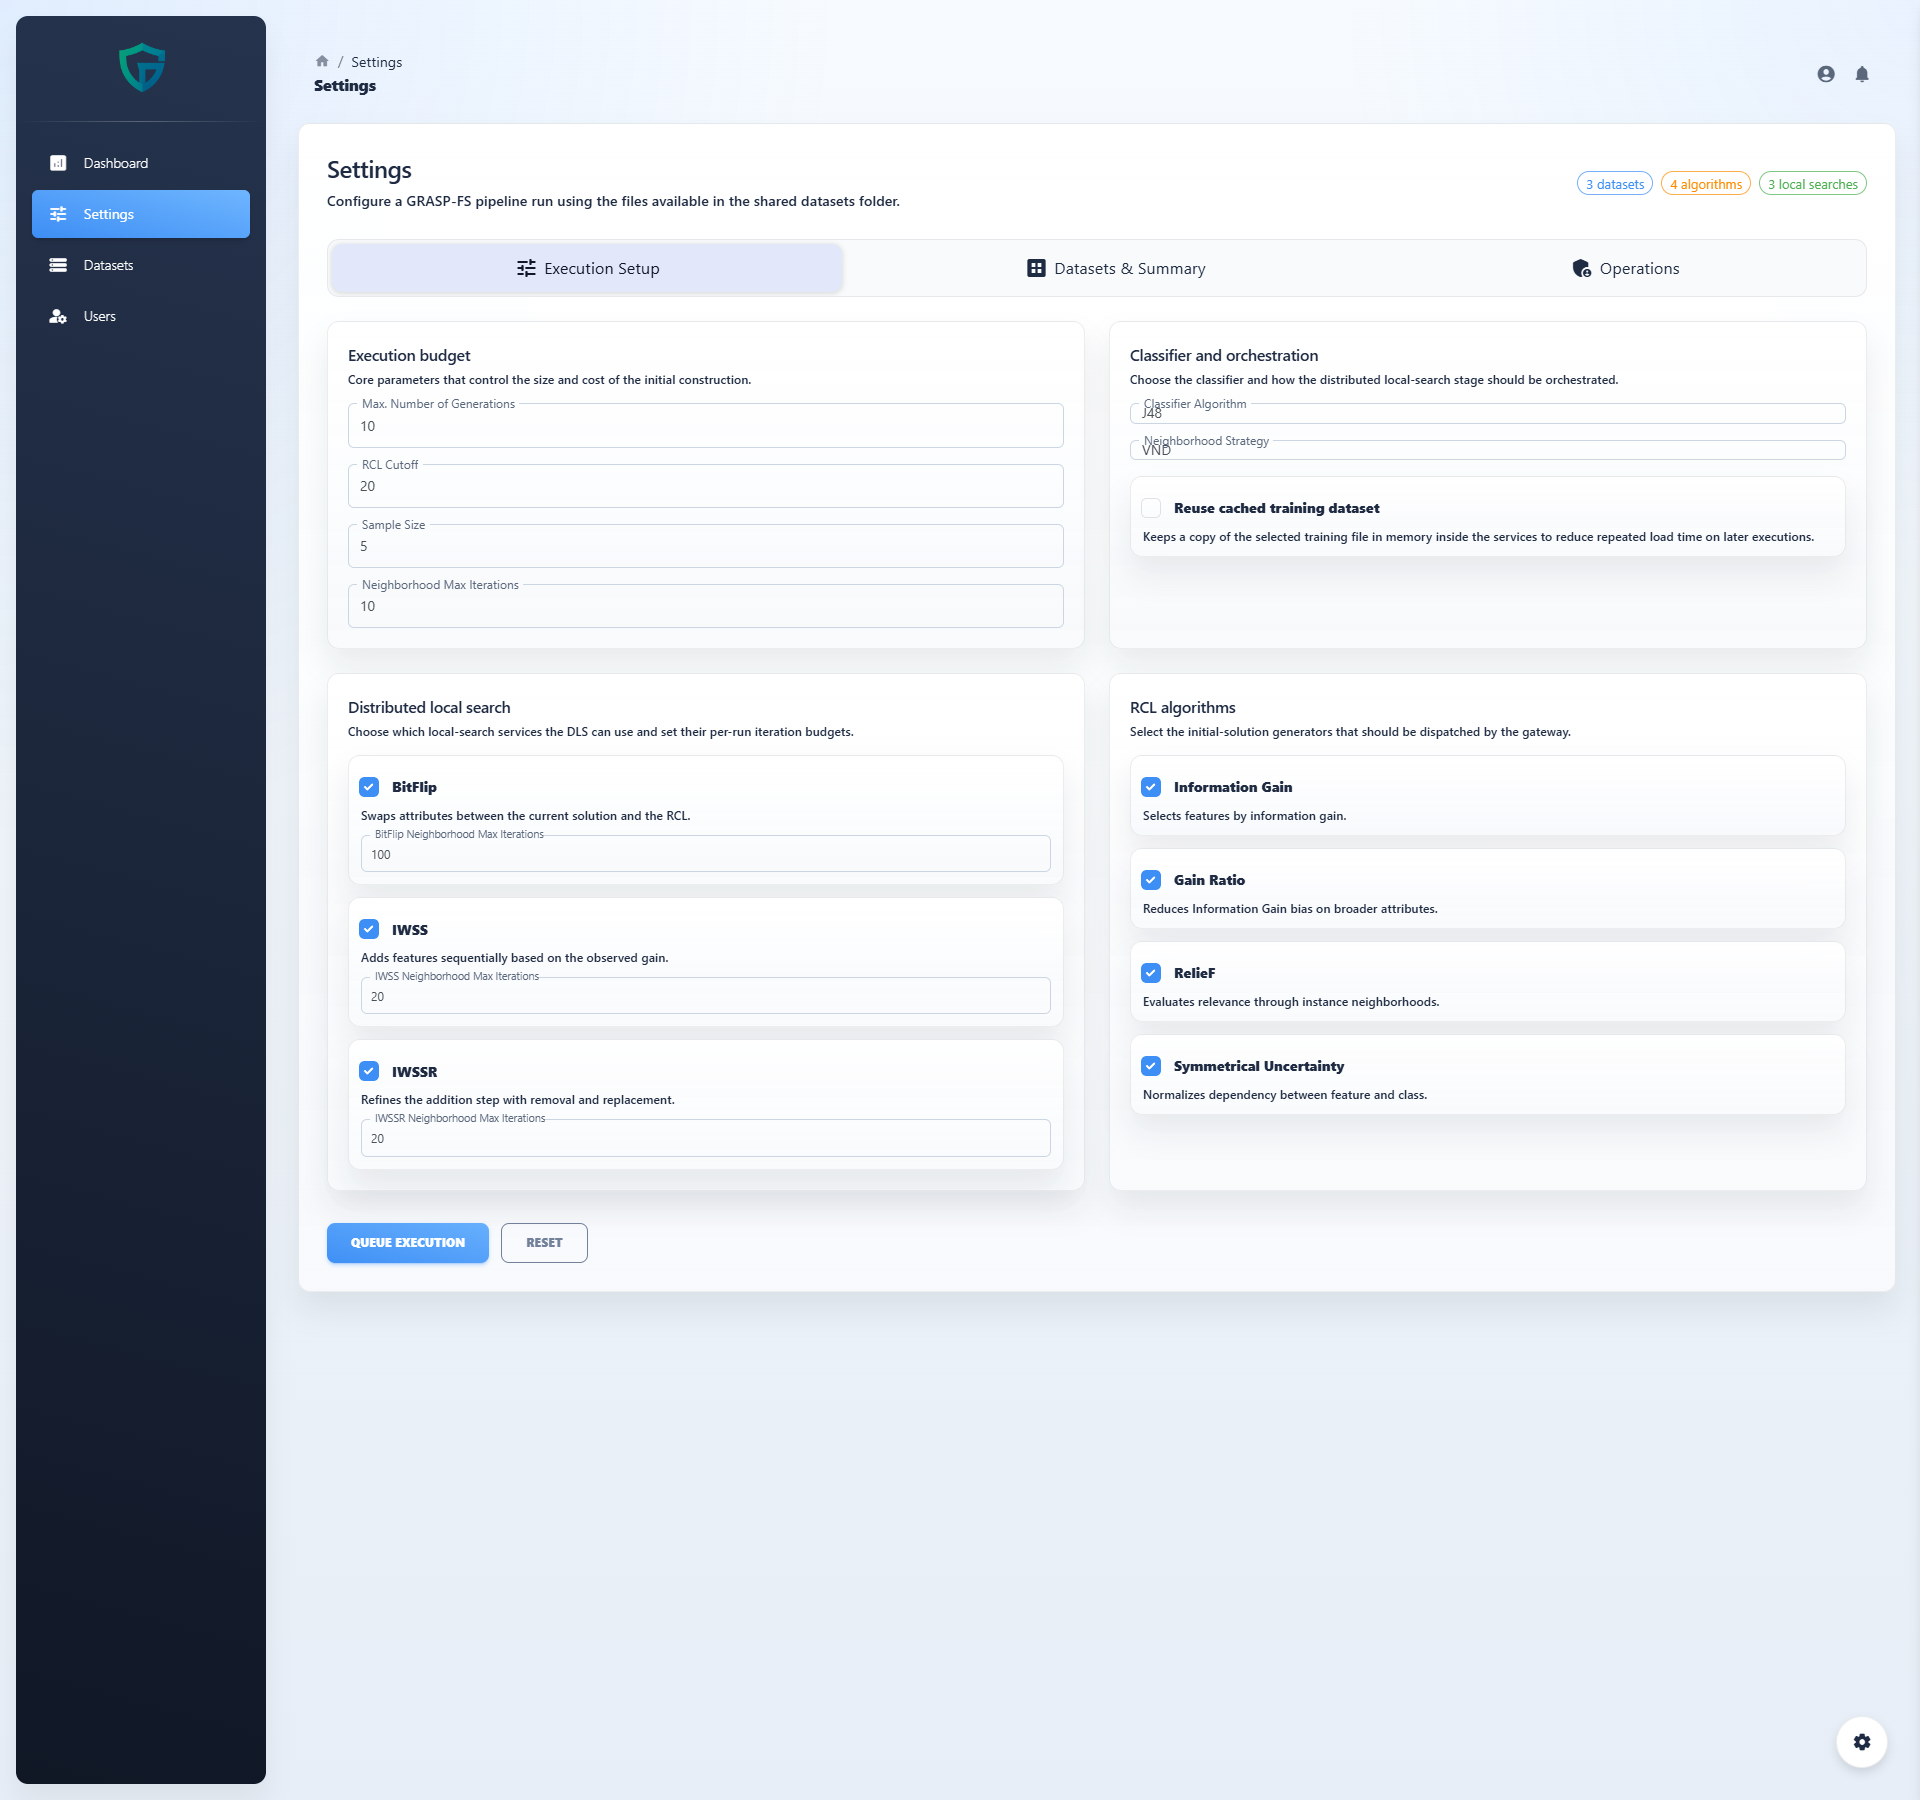
\includegraphics[width=\linewidth,height=0.80\textheight,keepaspectratio]{fig/front/15-settings-execution.png}
  \caption{Configuração de execução.}
  \label{fig:app-front-settings-execution}
\end{figure}

\begin{figure}[!htb]
  \centering
  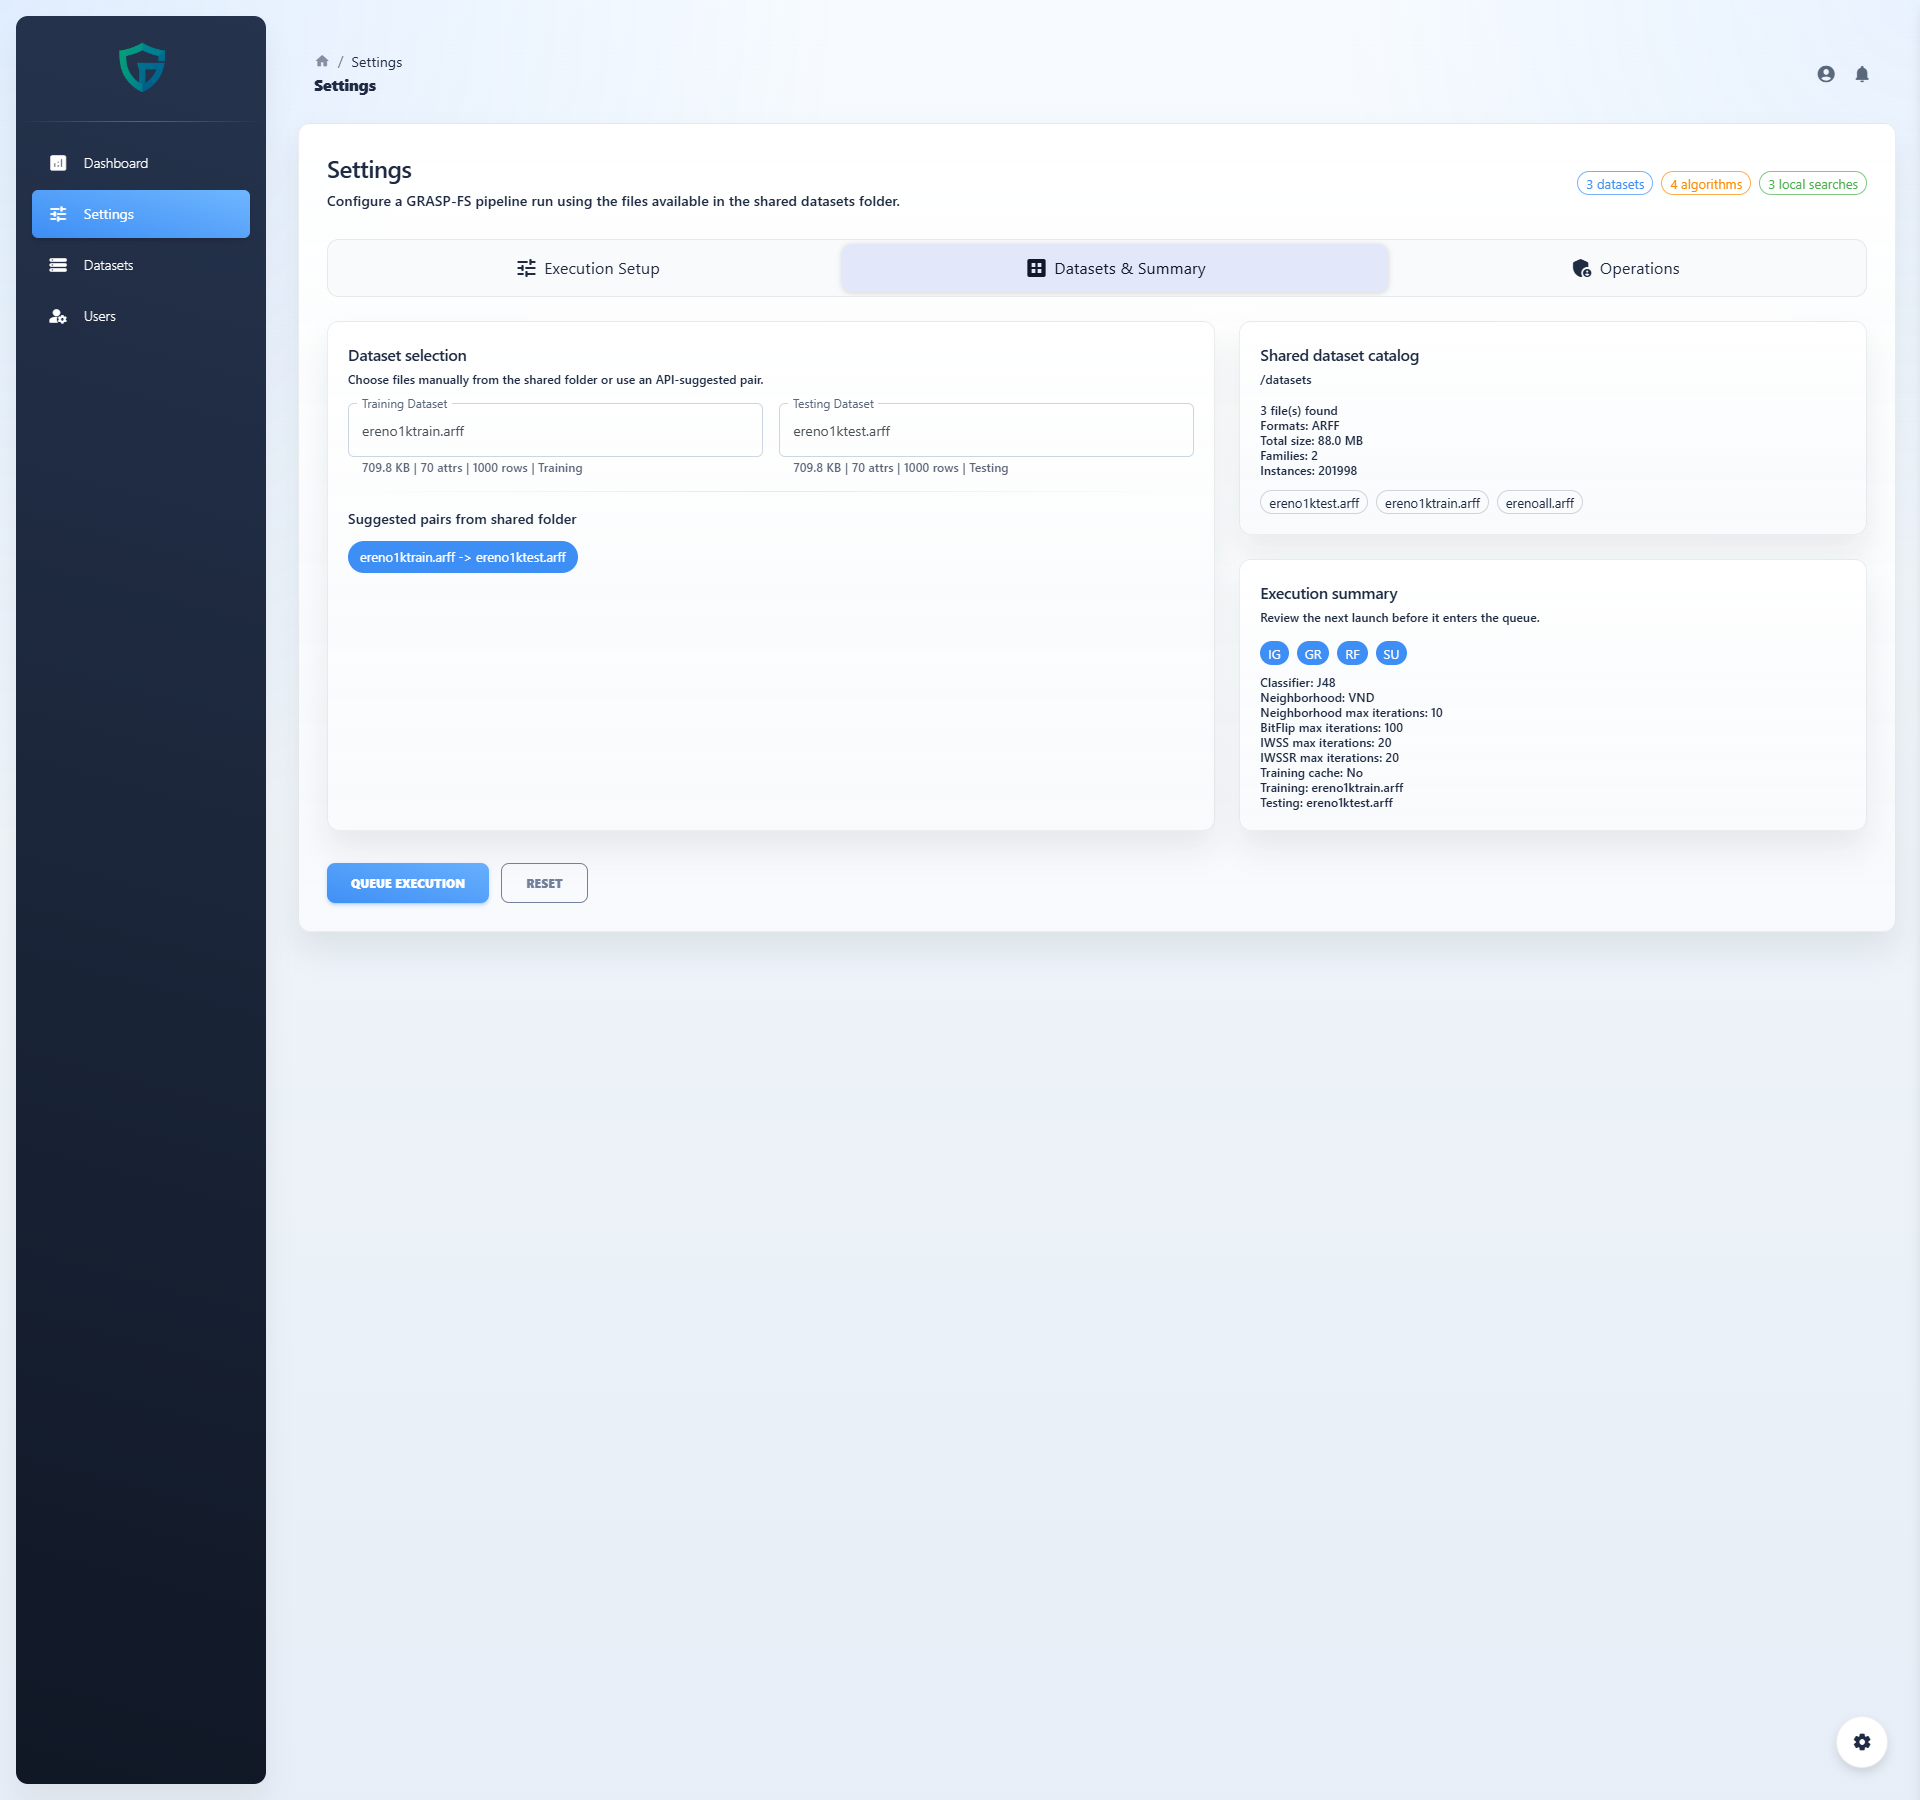
\includegraphics[width=\linewidth,height=0.80\textheight,keepaspectratio]{fig/front/16-settings-datasets.png}
  \caption{Configuração de conjuntos de dados.}
  \label{fig:app-front-settings-datasets}
\end{figure}

\begin{figure}[!htb]
  \centering
  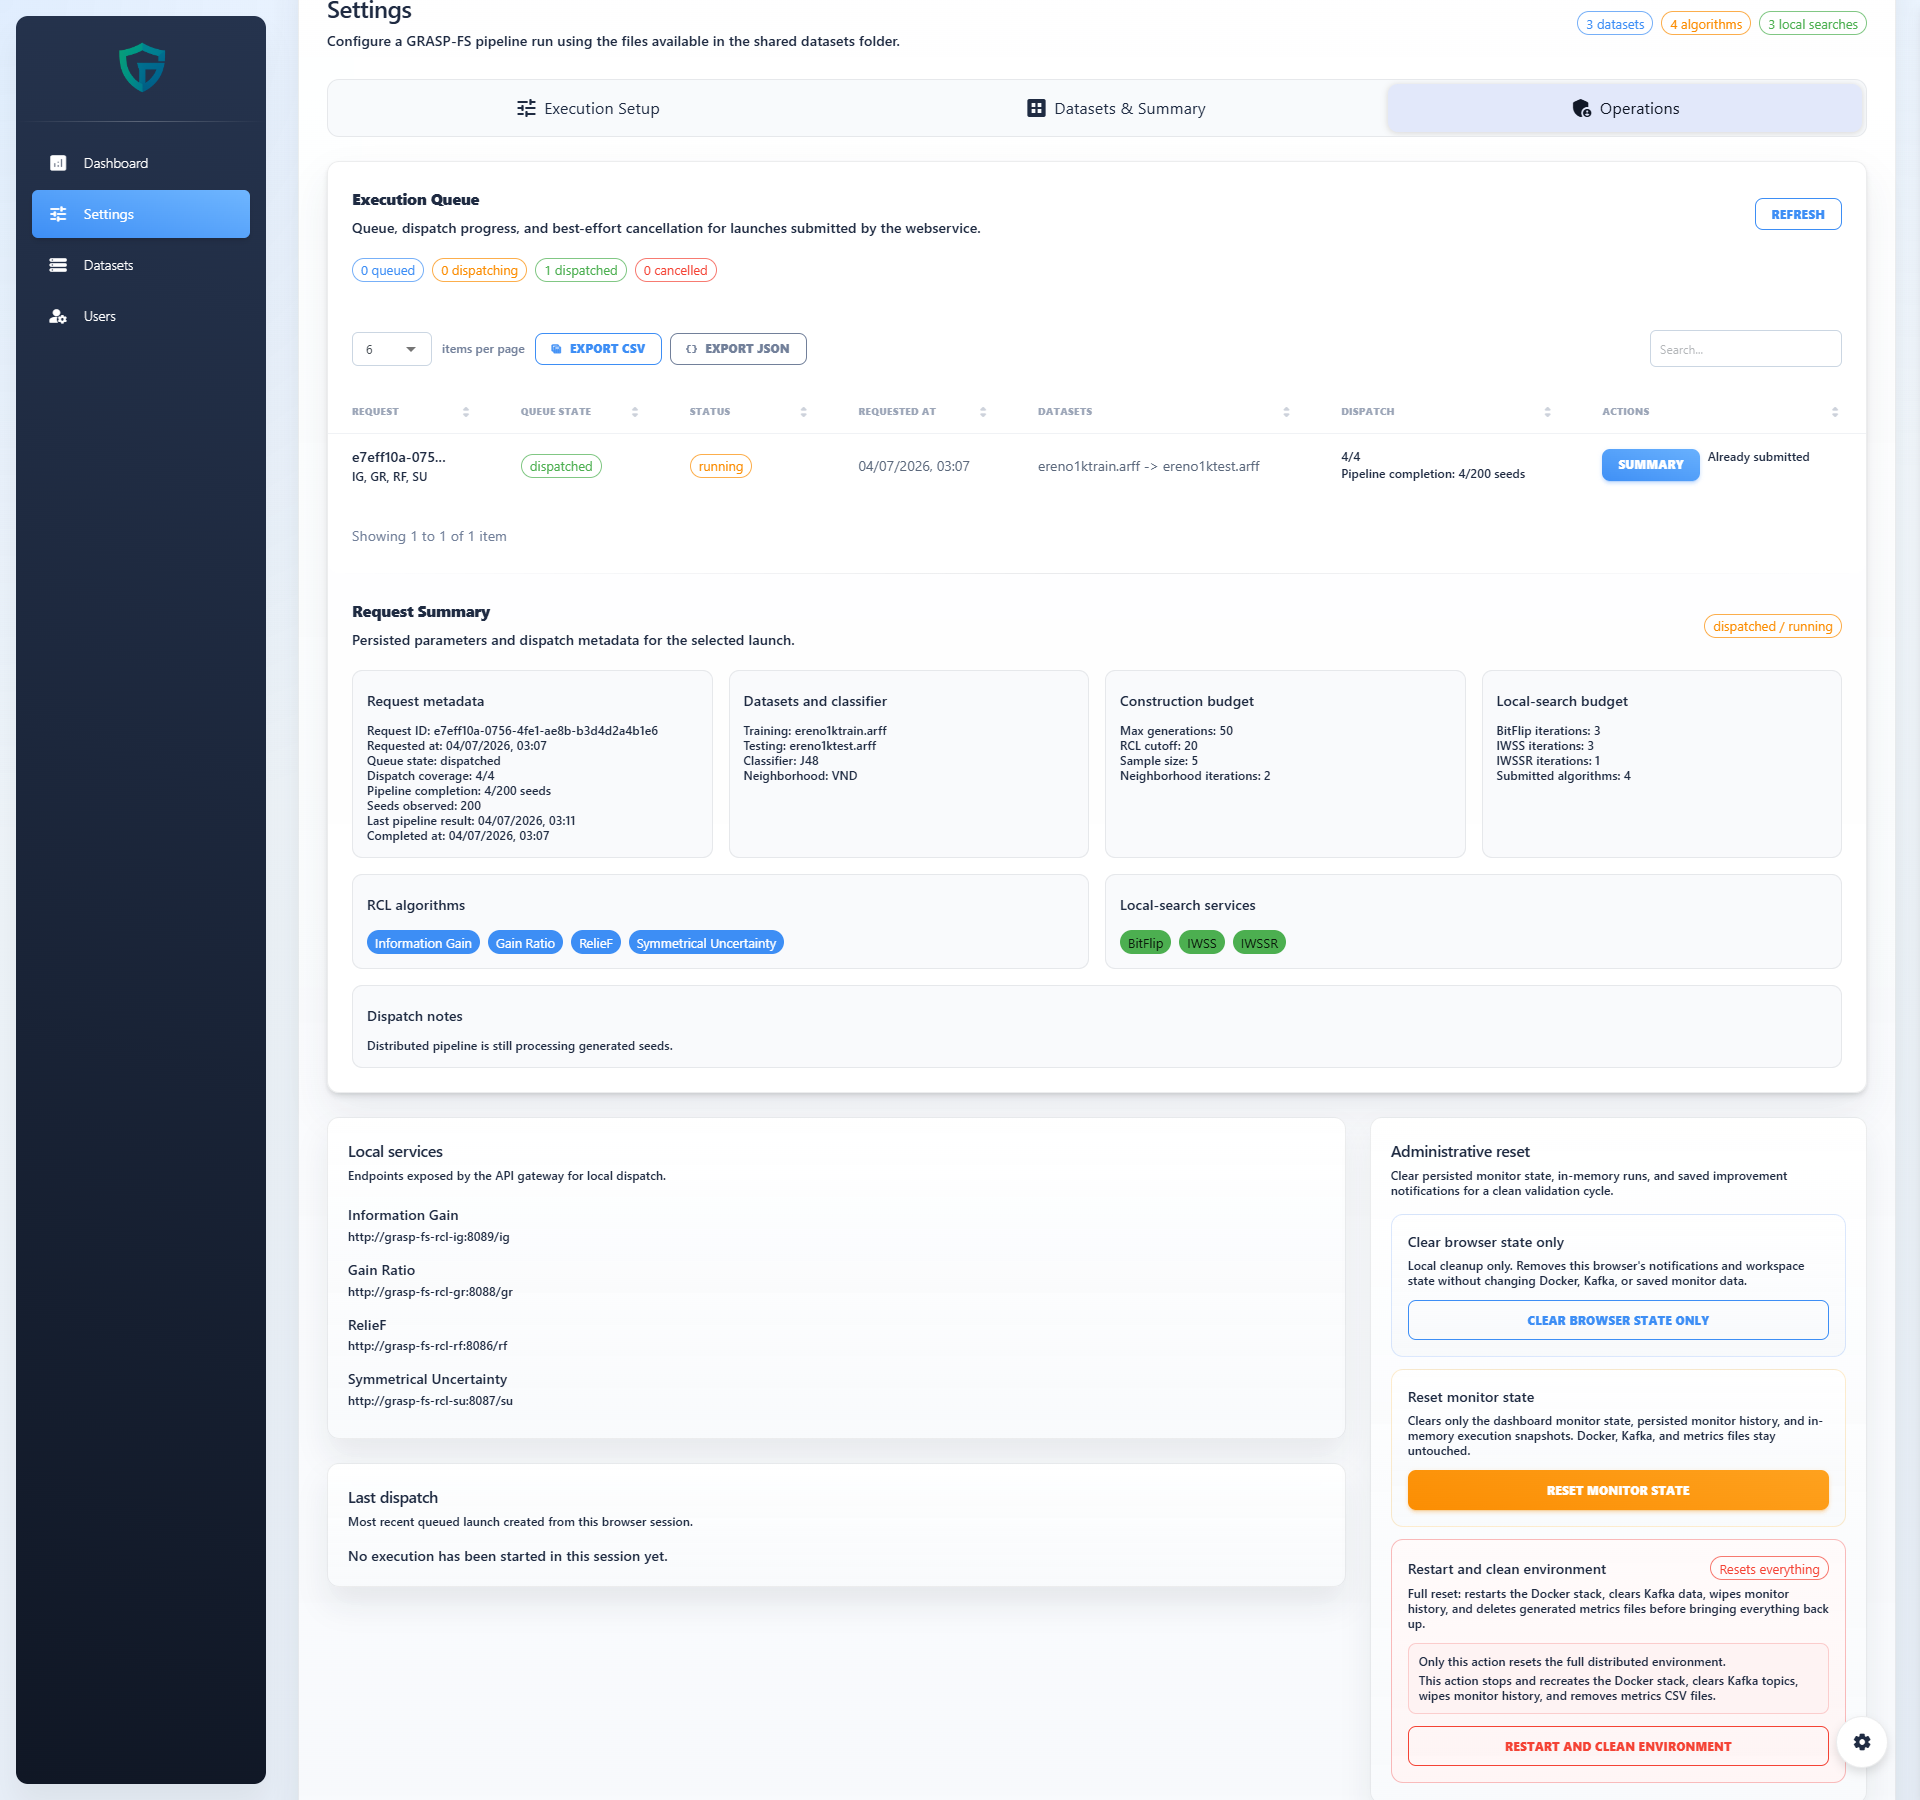
\includegraphics[width=\linewidth,height=0.80\textheight,keepaspectratio]{fig/front/17-settings-operations.png}
  \caption{Configuração de operações.}
  \label{fig:app-front-settings-operations}
\end{figure}

\begin{figure}[!htb]
  \centering
  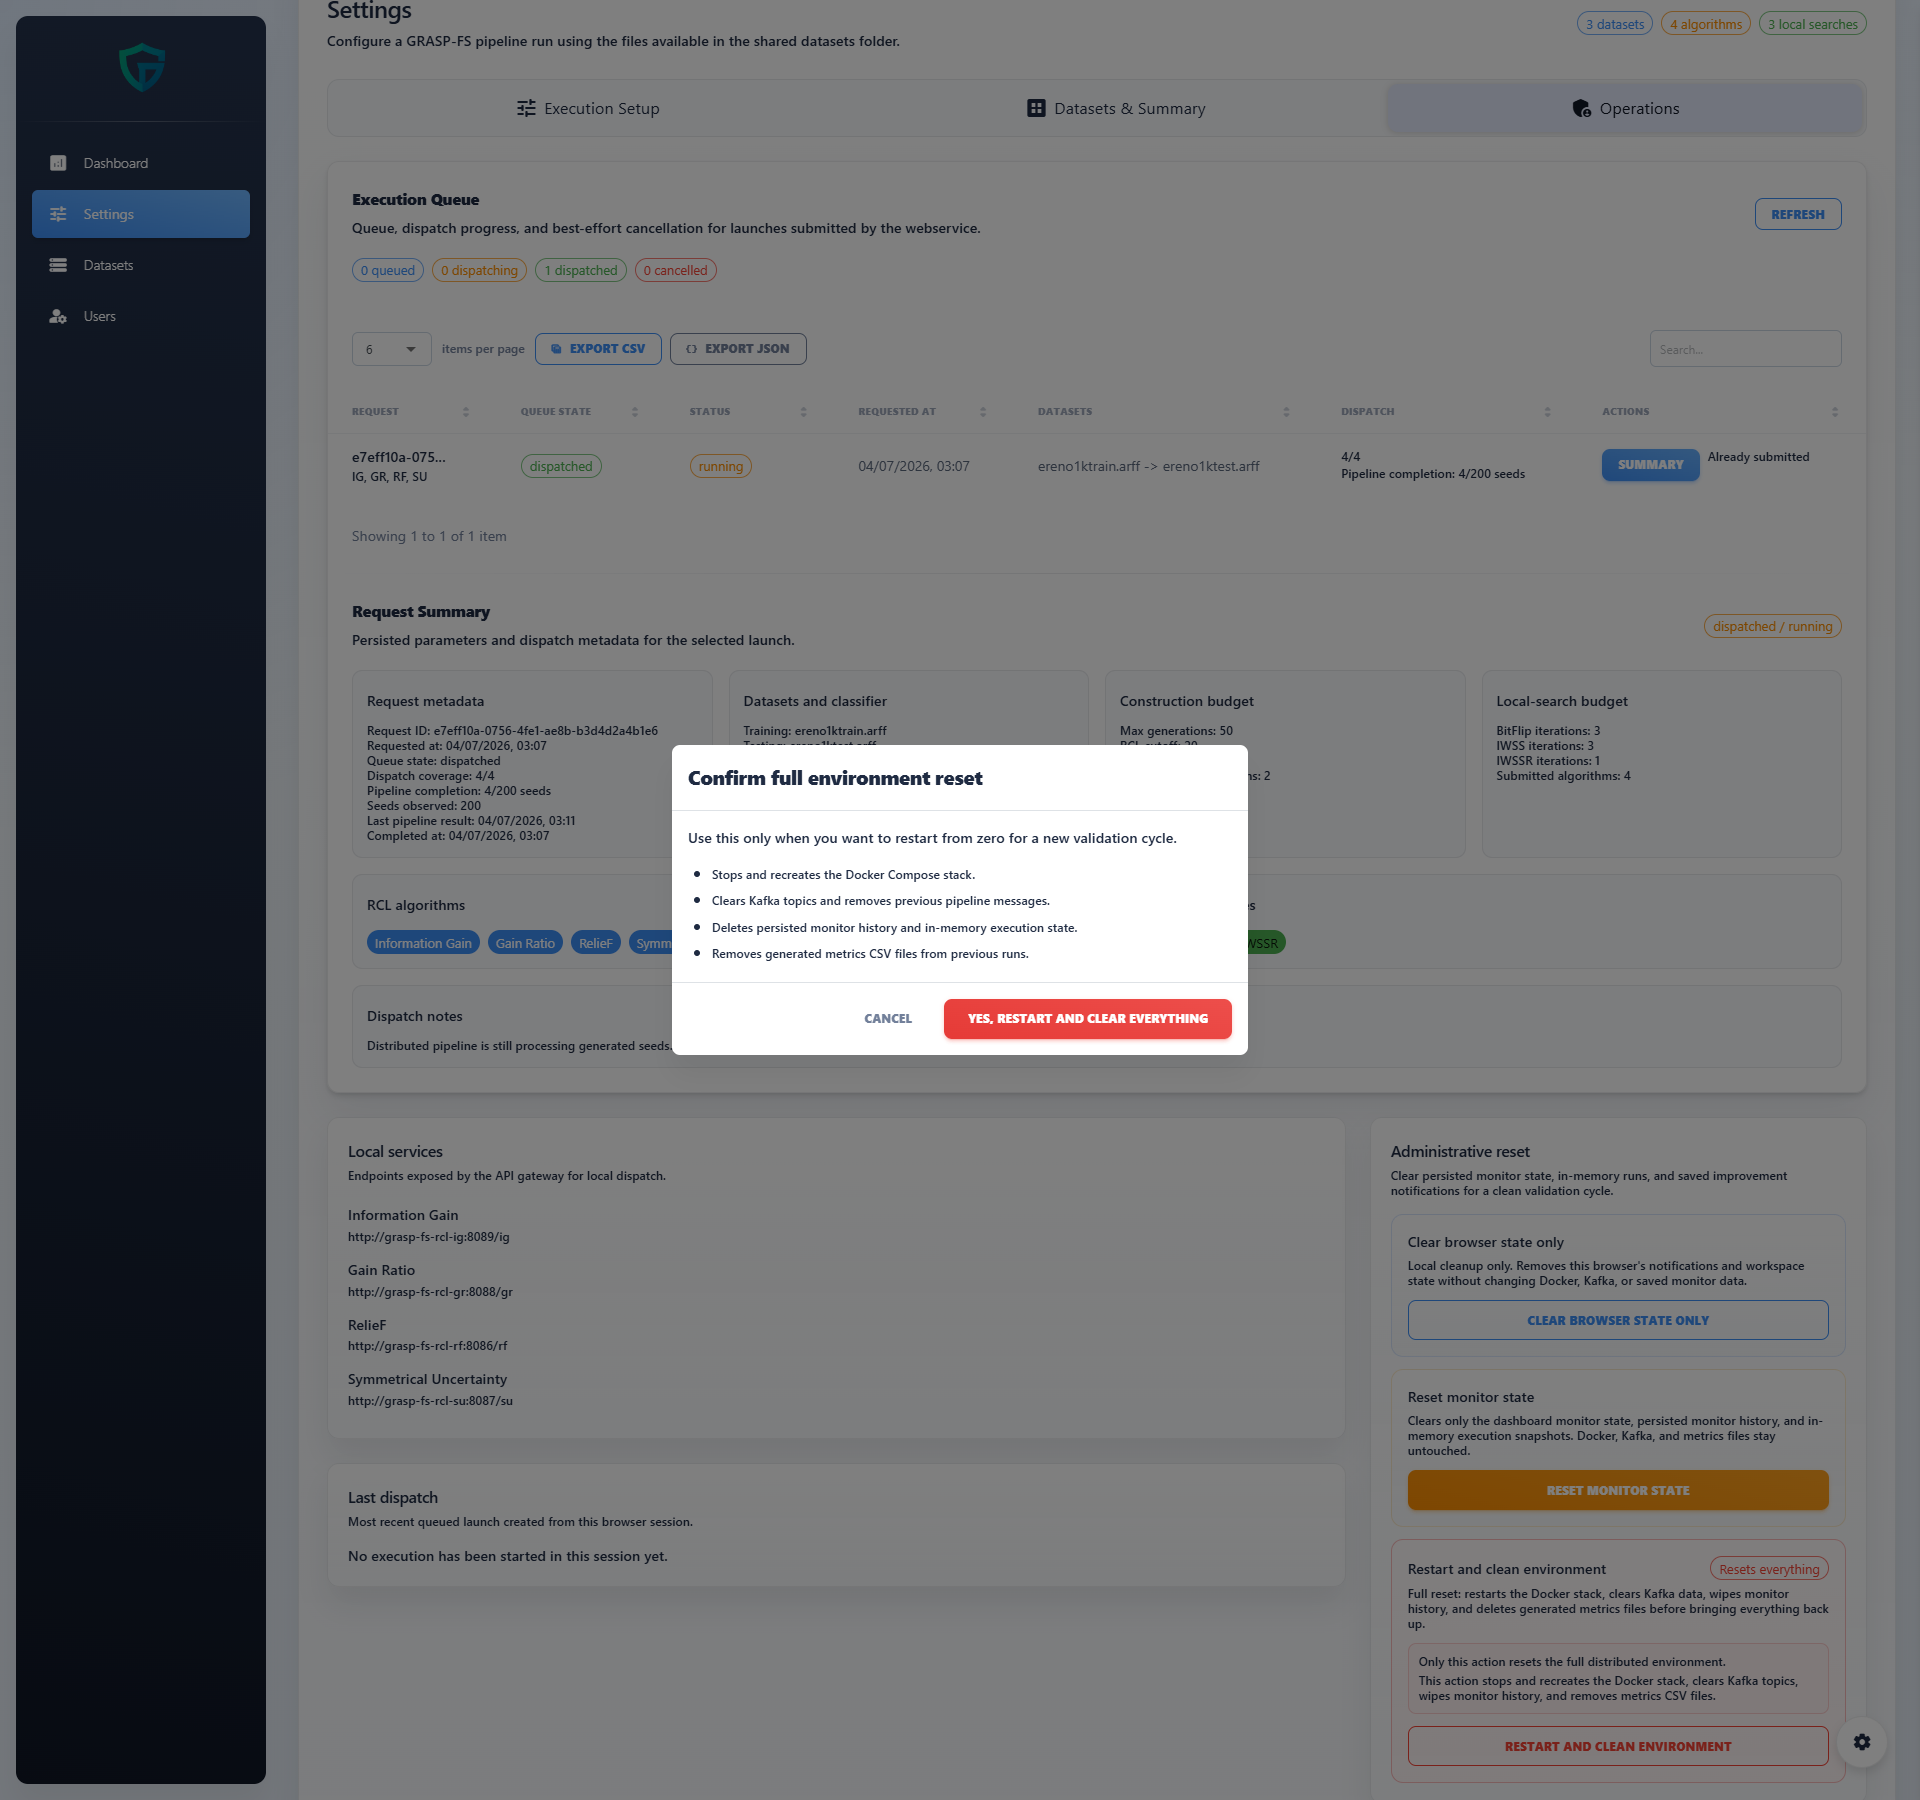
\includegraphics[width=\linewidth,height=0.80\textheight,keepaspectratio]{fig/front/18-settings-full-reset-dialog.png}
  \caption{Diálogo de reset completo.}
  \label{fig:app-front-settings-reset}
\end{figure}

\begin{figure}[!htb]
  \centering
  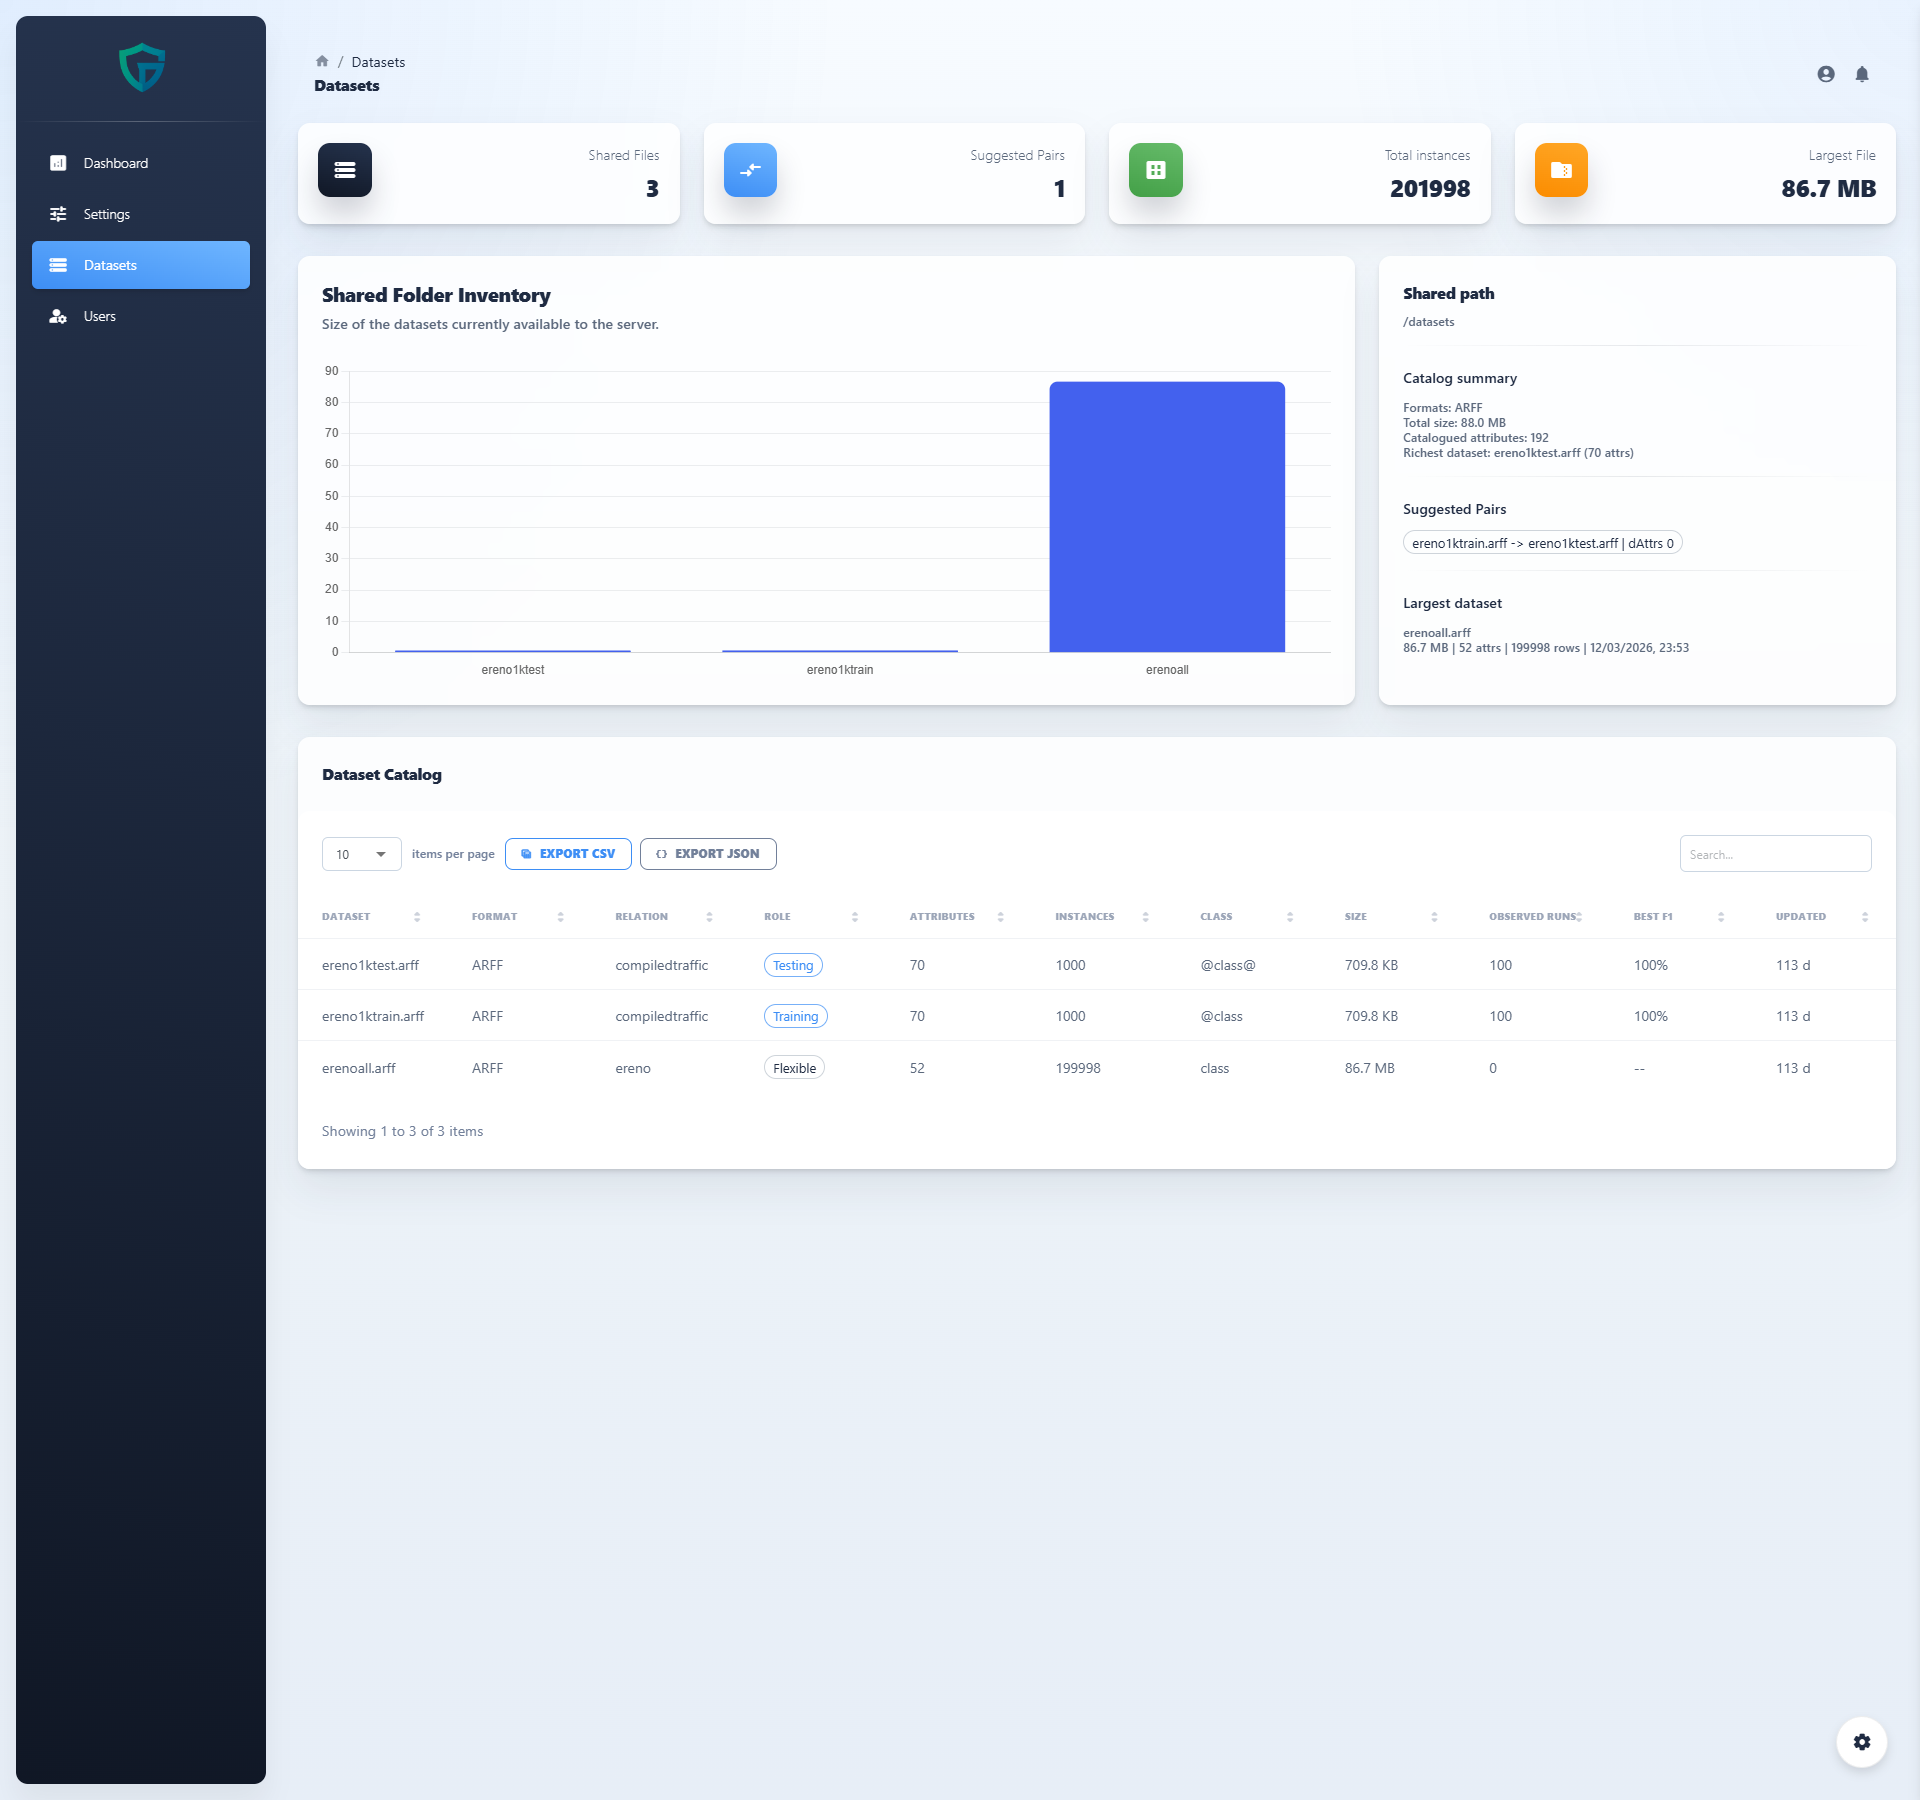
\includegraphics[width=\linewidth,height=0.80\textheight,keepaspectratio]{fig/front/19-datasets.png}
  \caption{Listagem de datasets.}
  \label{fig:app-front-datasets}
\end{figure}

\begin{figure}[!htb]
  \centering
  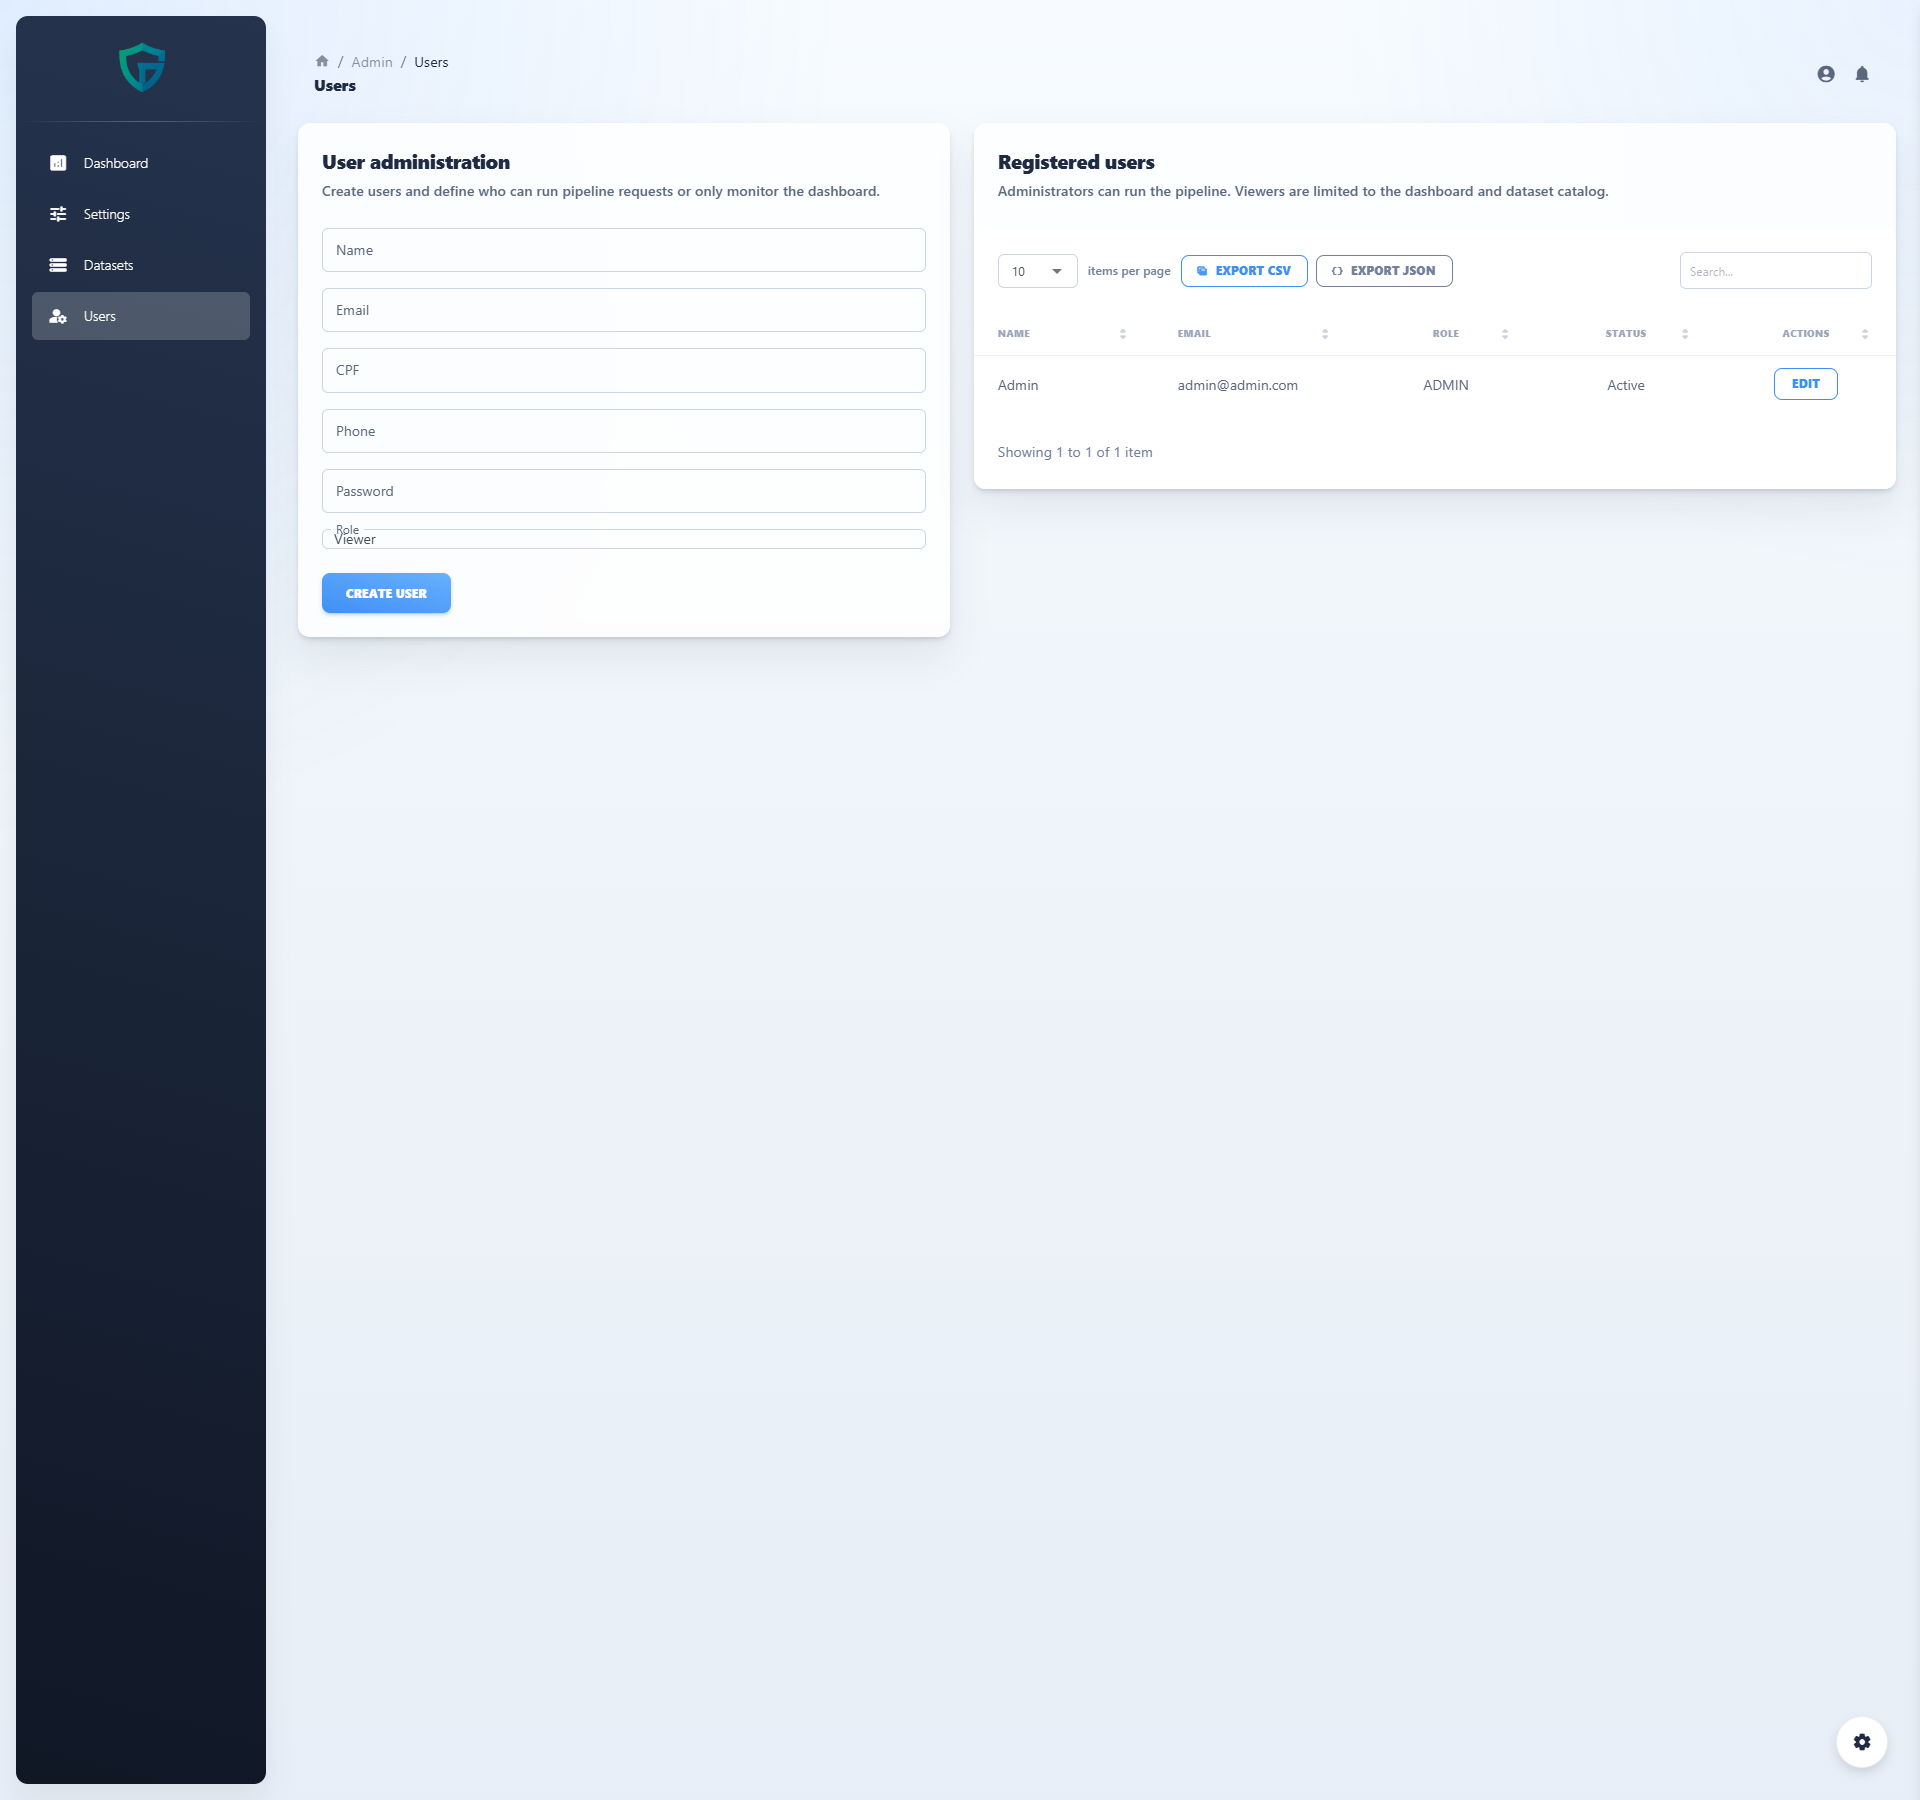
\includegraphics[width=\linewidth,height=0.80\textheight,keepaspectratio]{fig/front/20-users-list.png}
  \caption{Listagem de usuários.}
  \label{fig:app-front-users-list}
\end{figure}

\begin{figure}[!htb]
  \centering
  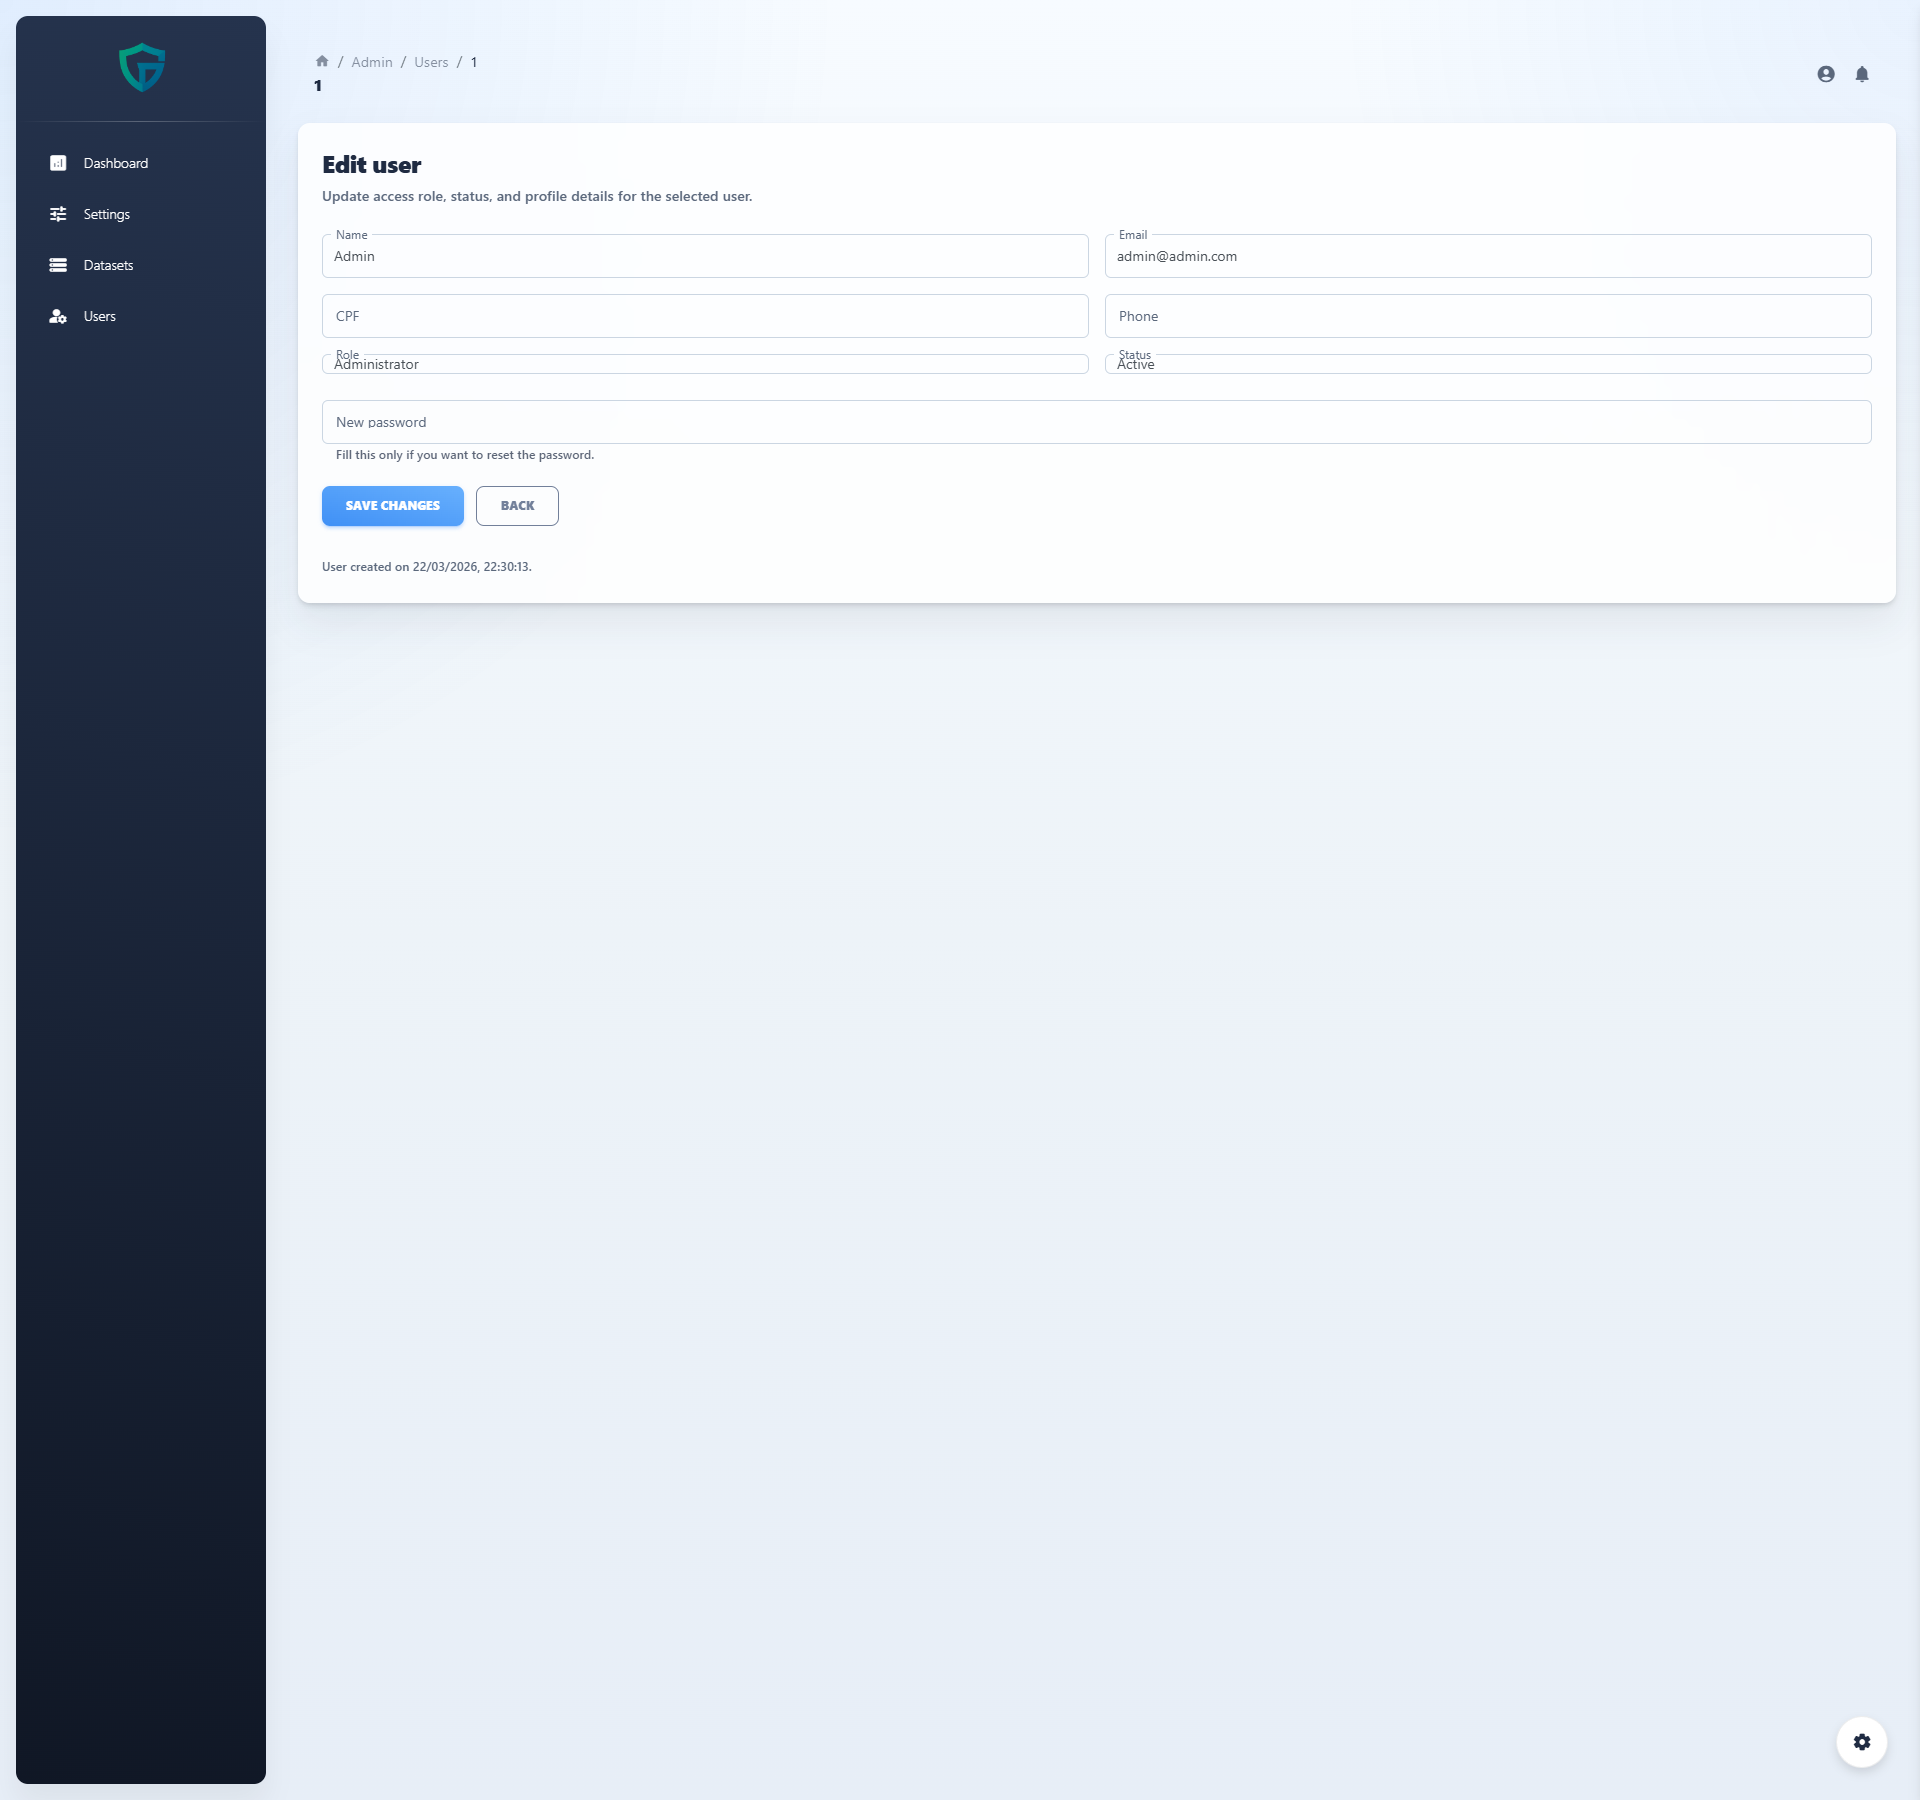
\includegraphics[width=\linewidth,height=0.80\textheight,keepaspectratio]{fig/front/21-user-edit.png}
  \caption{Edição de usuário.}
  \label{fig:app-front-user-edit}
\end{figure}

\chapter{Vídeo e Documentação}
\label{app:video-docs}

O vídeo demonstrativo da plataforma foi incluído como apoio à defesa. Como arquivos MP4 nem sempre são renderizados diretamente pelo leitor de PDF, o material é disponibilizado por link e também mantido na pasta de figuras do projeto.
O poster ajuda a identificar rapidamente o conteúdo do vídeo mesmo quando o PDF é acessado em um visualizador que não embute mídia.
As Figuras~\ref{fig:app-front-video-poster} e~\ref{fig:app-backend-swagger} completam o material de apoio com a demonstração e a documentação da API.

\begin{figure}[!htb]
  \centering
  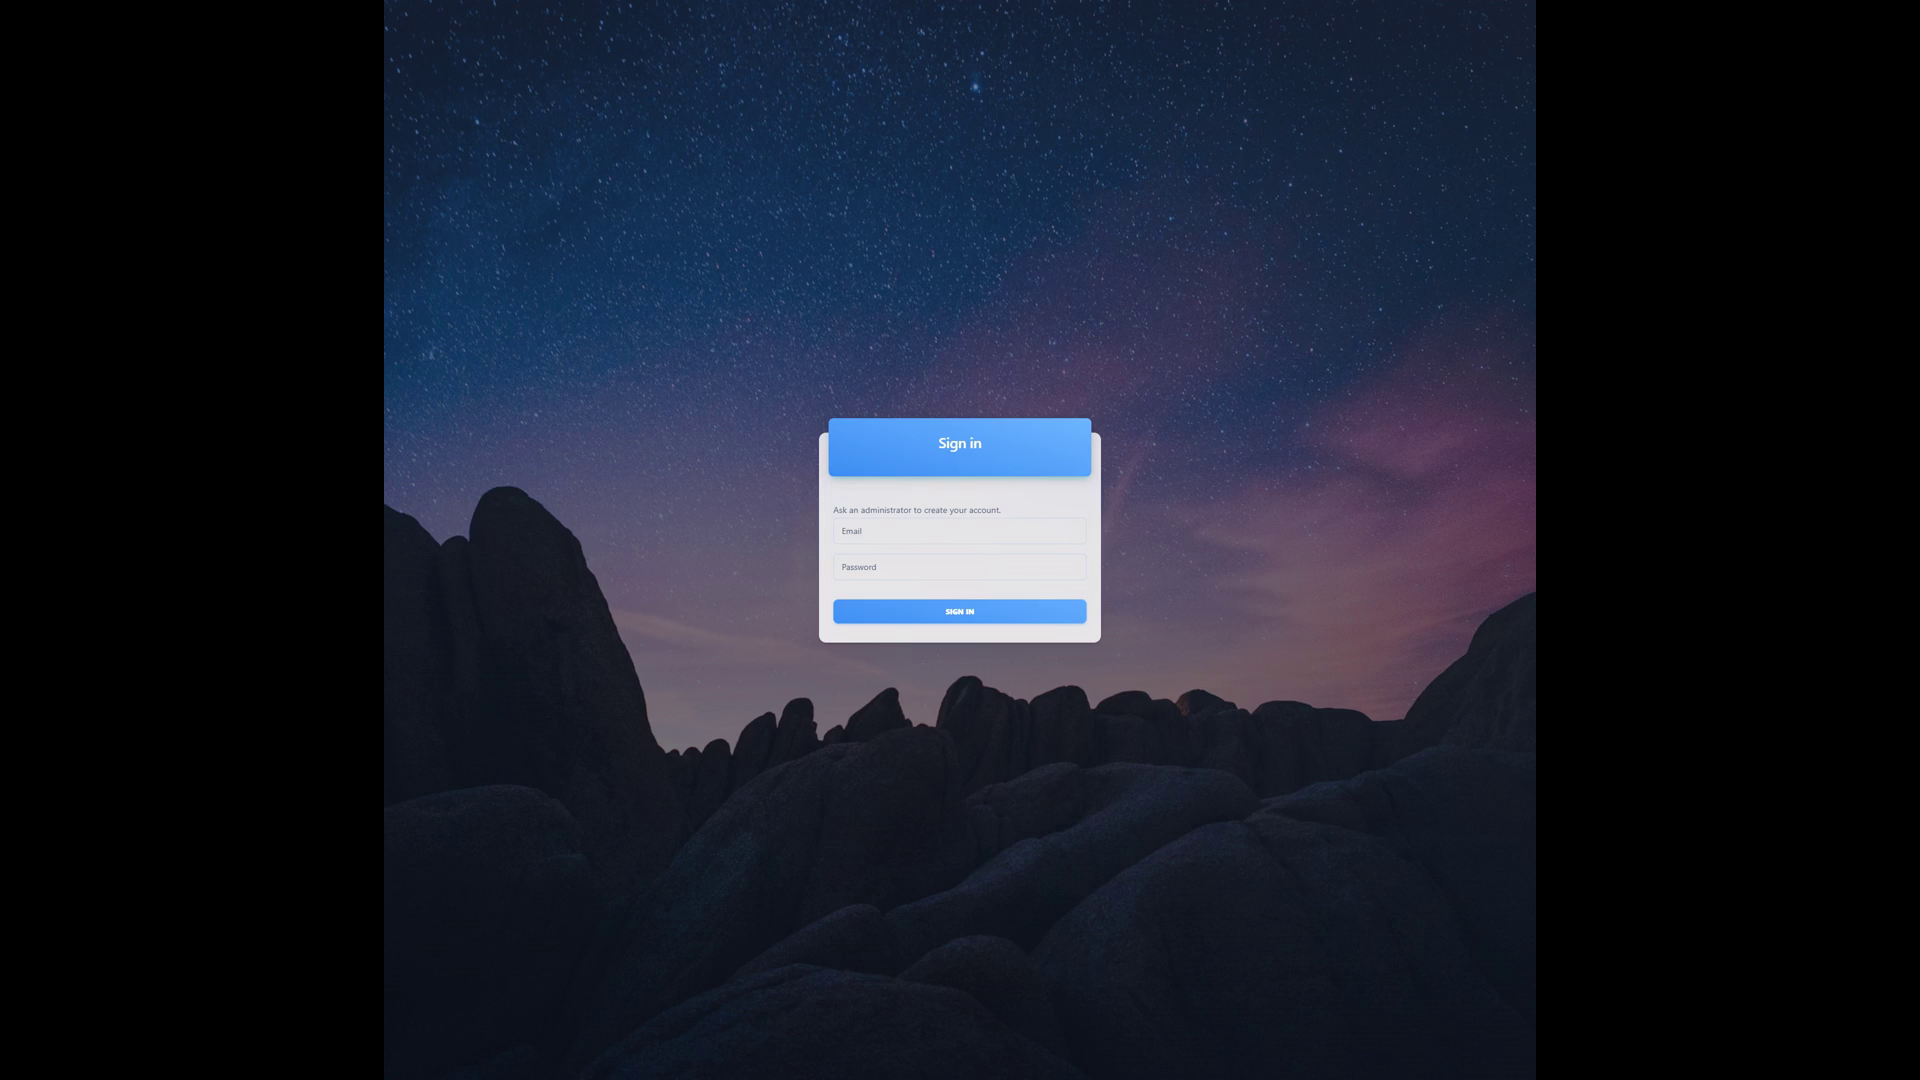
\includegraphics[width=.82\linewidth]{fig/front/site-walkthrough-hd-poster.png}
  \caption{Poster do vídeo demonstrativo da plataforma.}
  \label{fig:app-front-video-poster}
\end{figure}

\noindent\textbf{Vídeo demonstrativo:} \url{https://youtu.be/-uqZPaTOjsU}

\vspace{1em}
\noindent O vídeo de demonstração deve ser disponibilizado em um repositório ou artefato persistente, identificado pela versão correspondente à dissertação.

\begin{figure}[!htb]
  \centering
  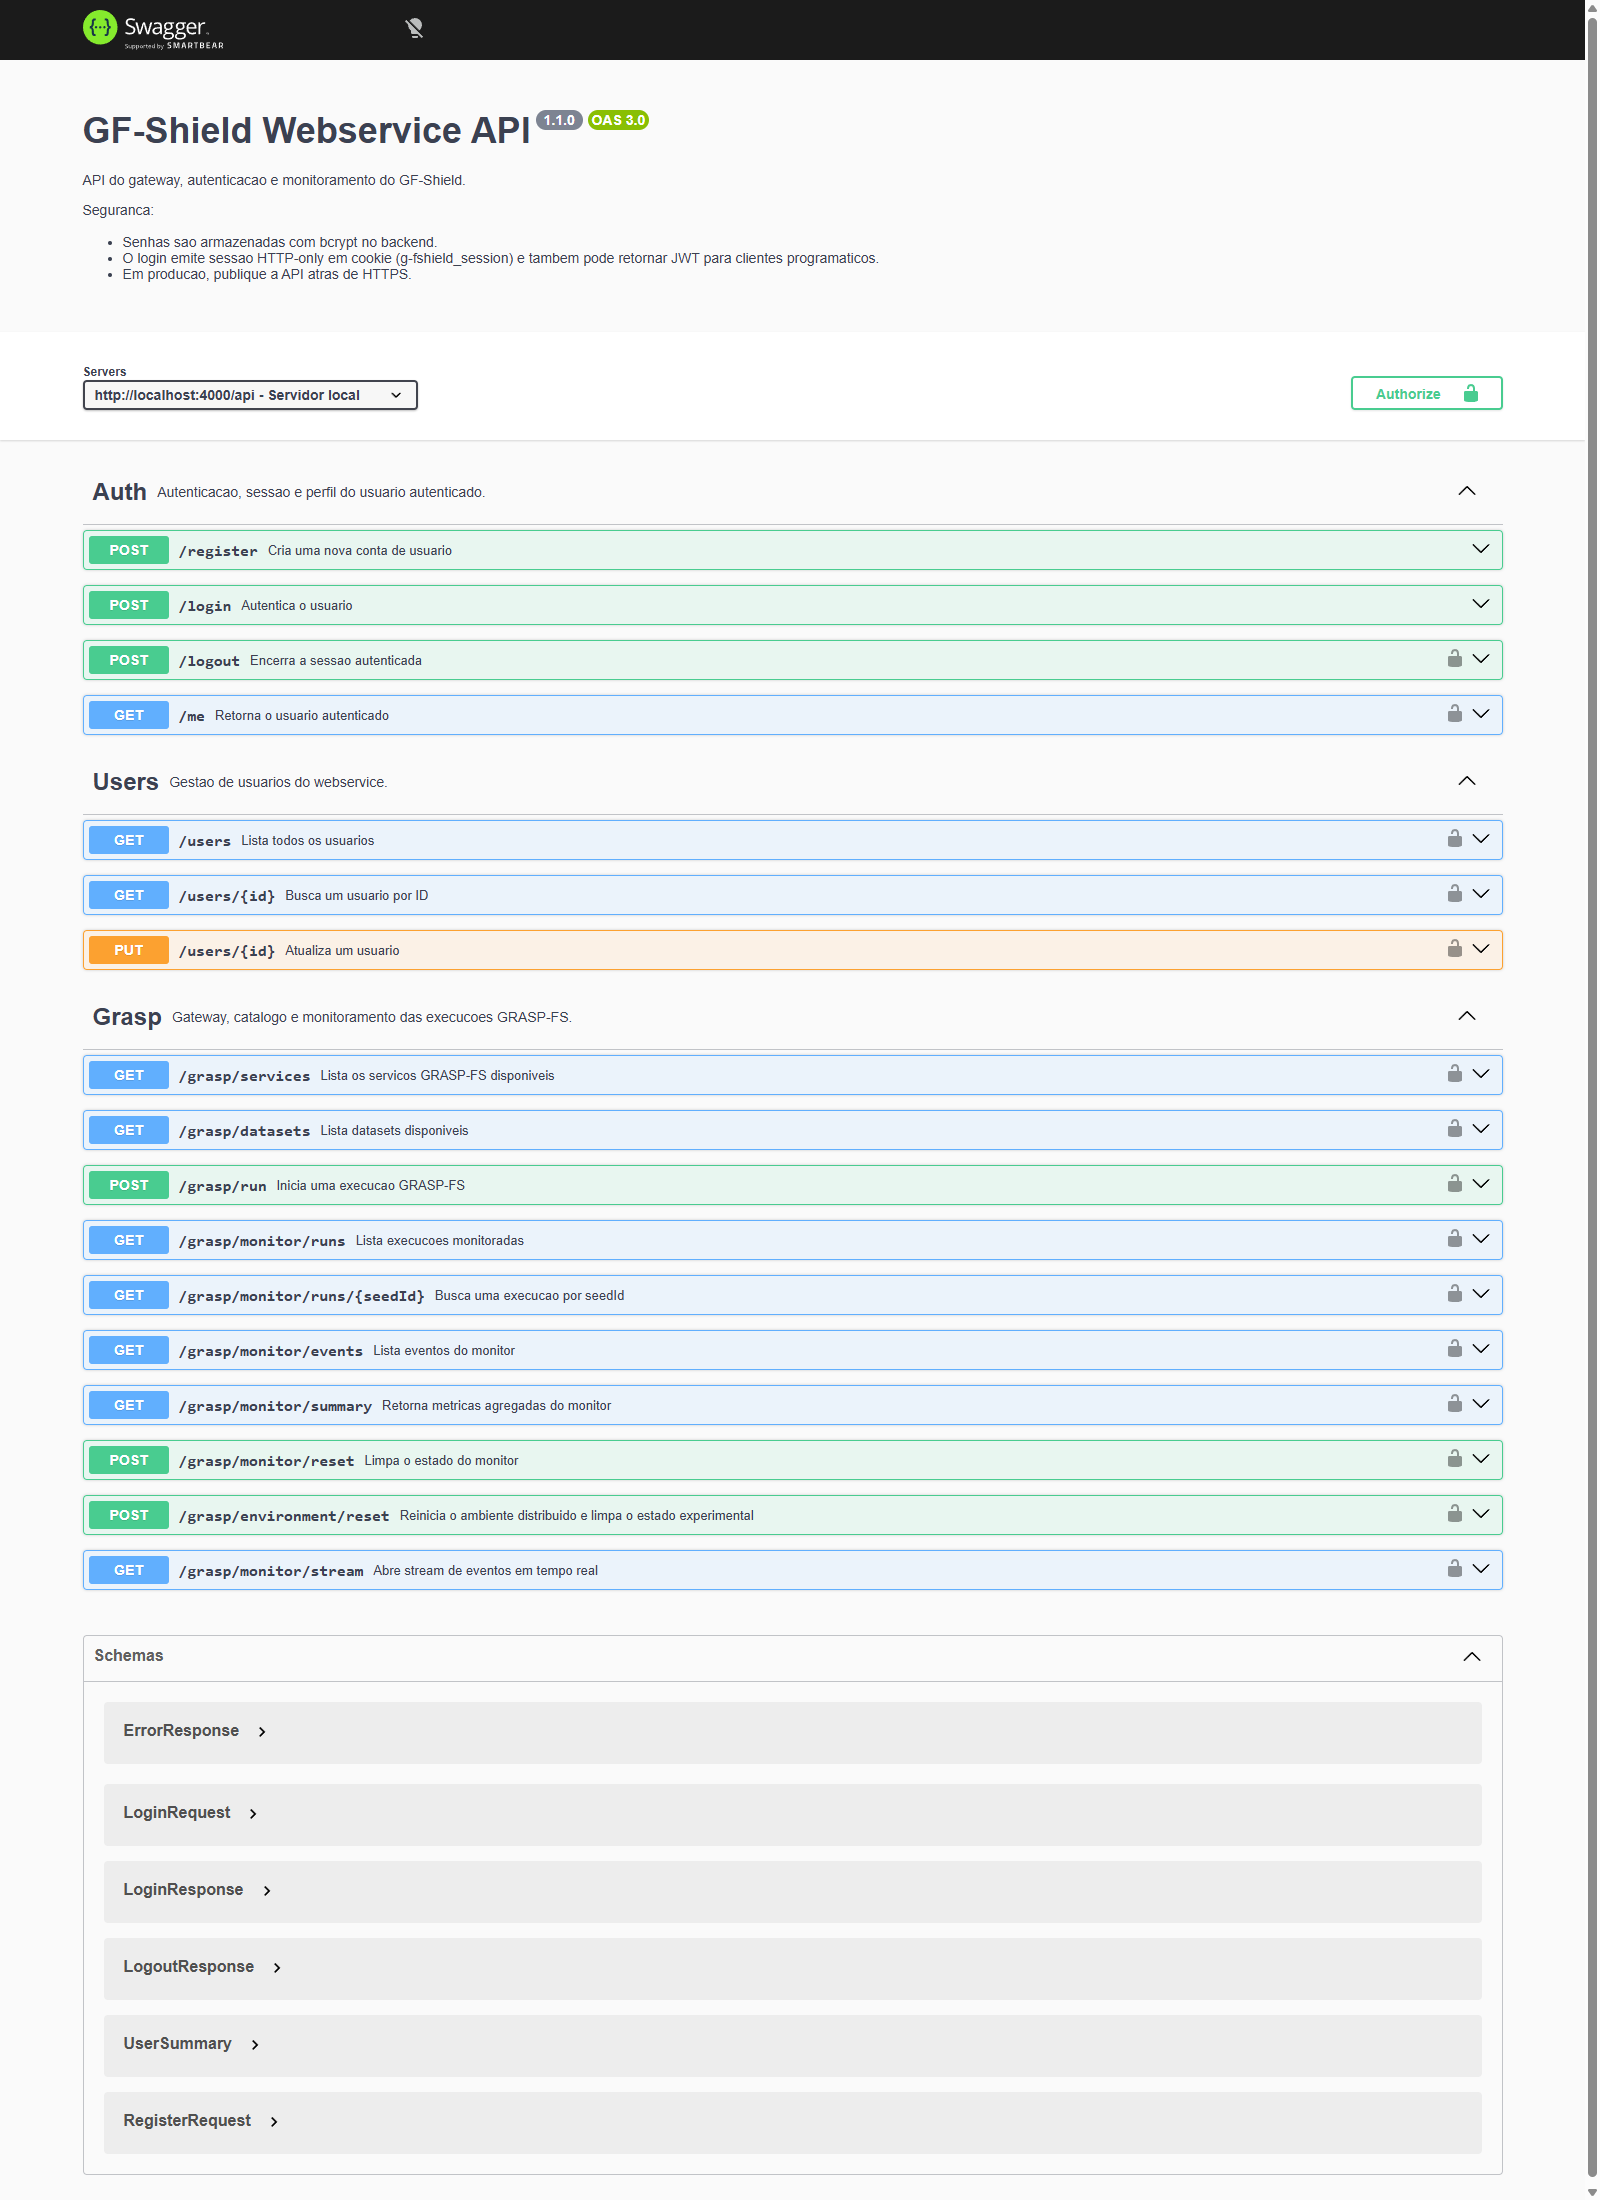
\includegraphics[width=.72\linewidth]{fig/front/swagger-api-docs.png}
  \caption{Documentação Swagger da API do backend.}
  \label{fig:app-backend-swagger}
\end{figure}

\chapter{Diagramas de Arquitetura}
\label{app:diagrams}

Este apêndice reúne os diagramas específicos que complementam a leitura da arquitetura principal.
Eles foram incluídos para conectar o material visual do desenvolvimento às telas e aos fluxos operacionais mostrados nas demais seções.
As Figuras~\ref{fig:app-front-flow},~\ref{fig:app-backend-architecture},~\ref{fig:app-drg-generic} e~\ref{fig:app-architecture-summary} mostram a cadeia arquitetural completa.

\begin{figure}[!htb]
  \centering
  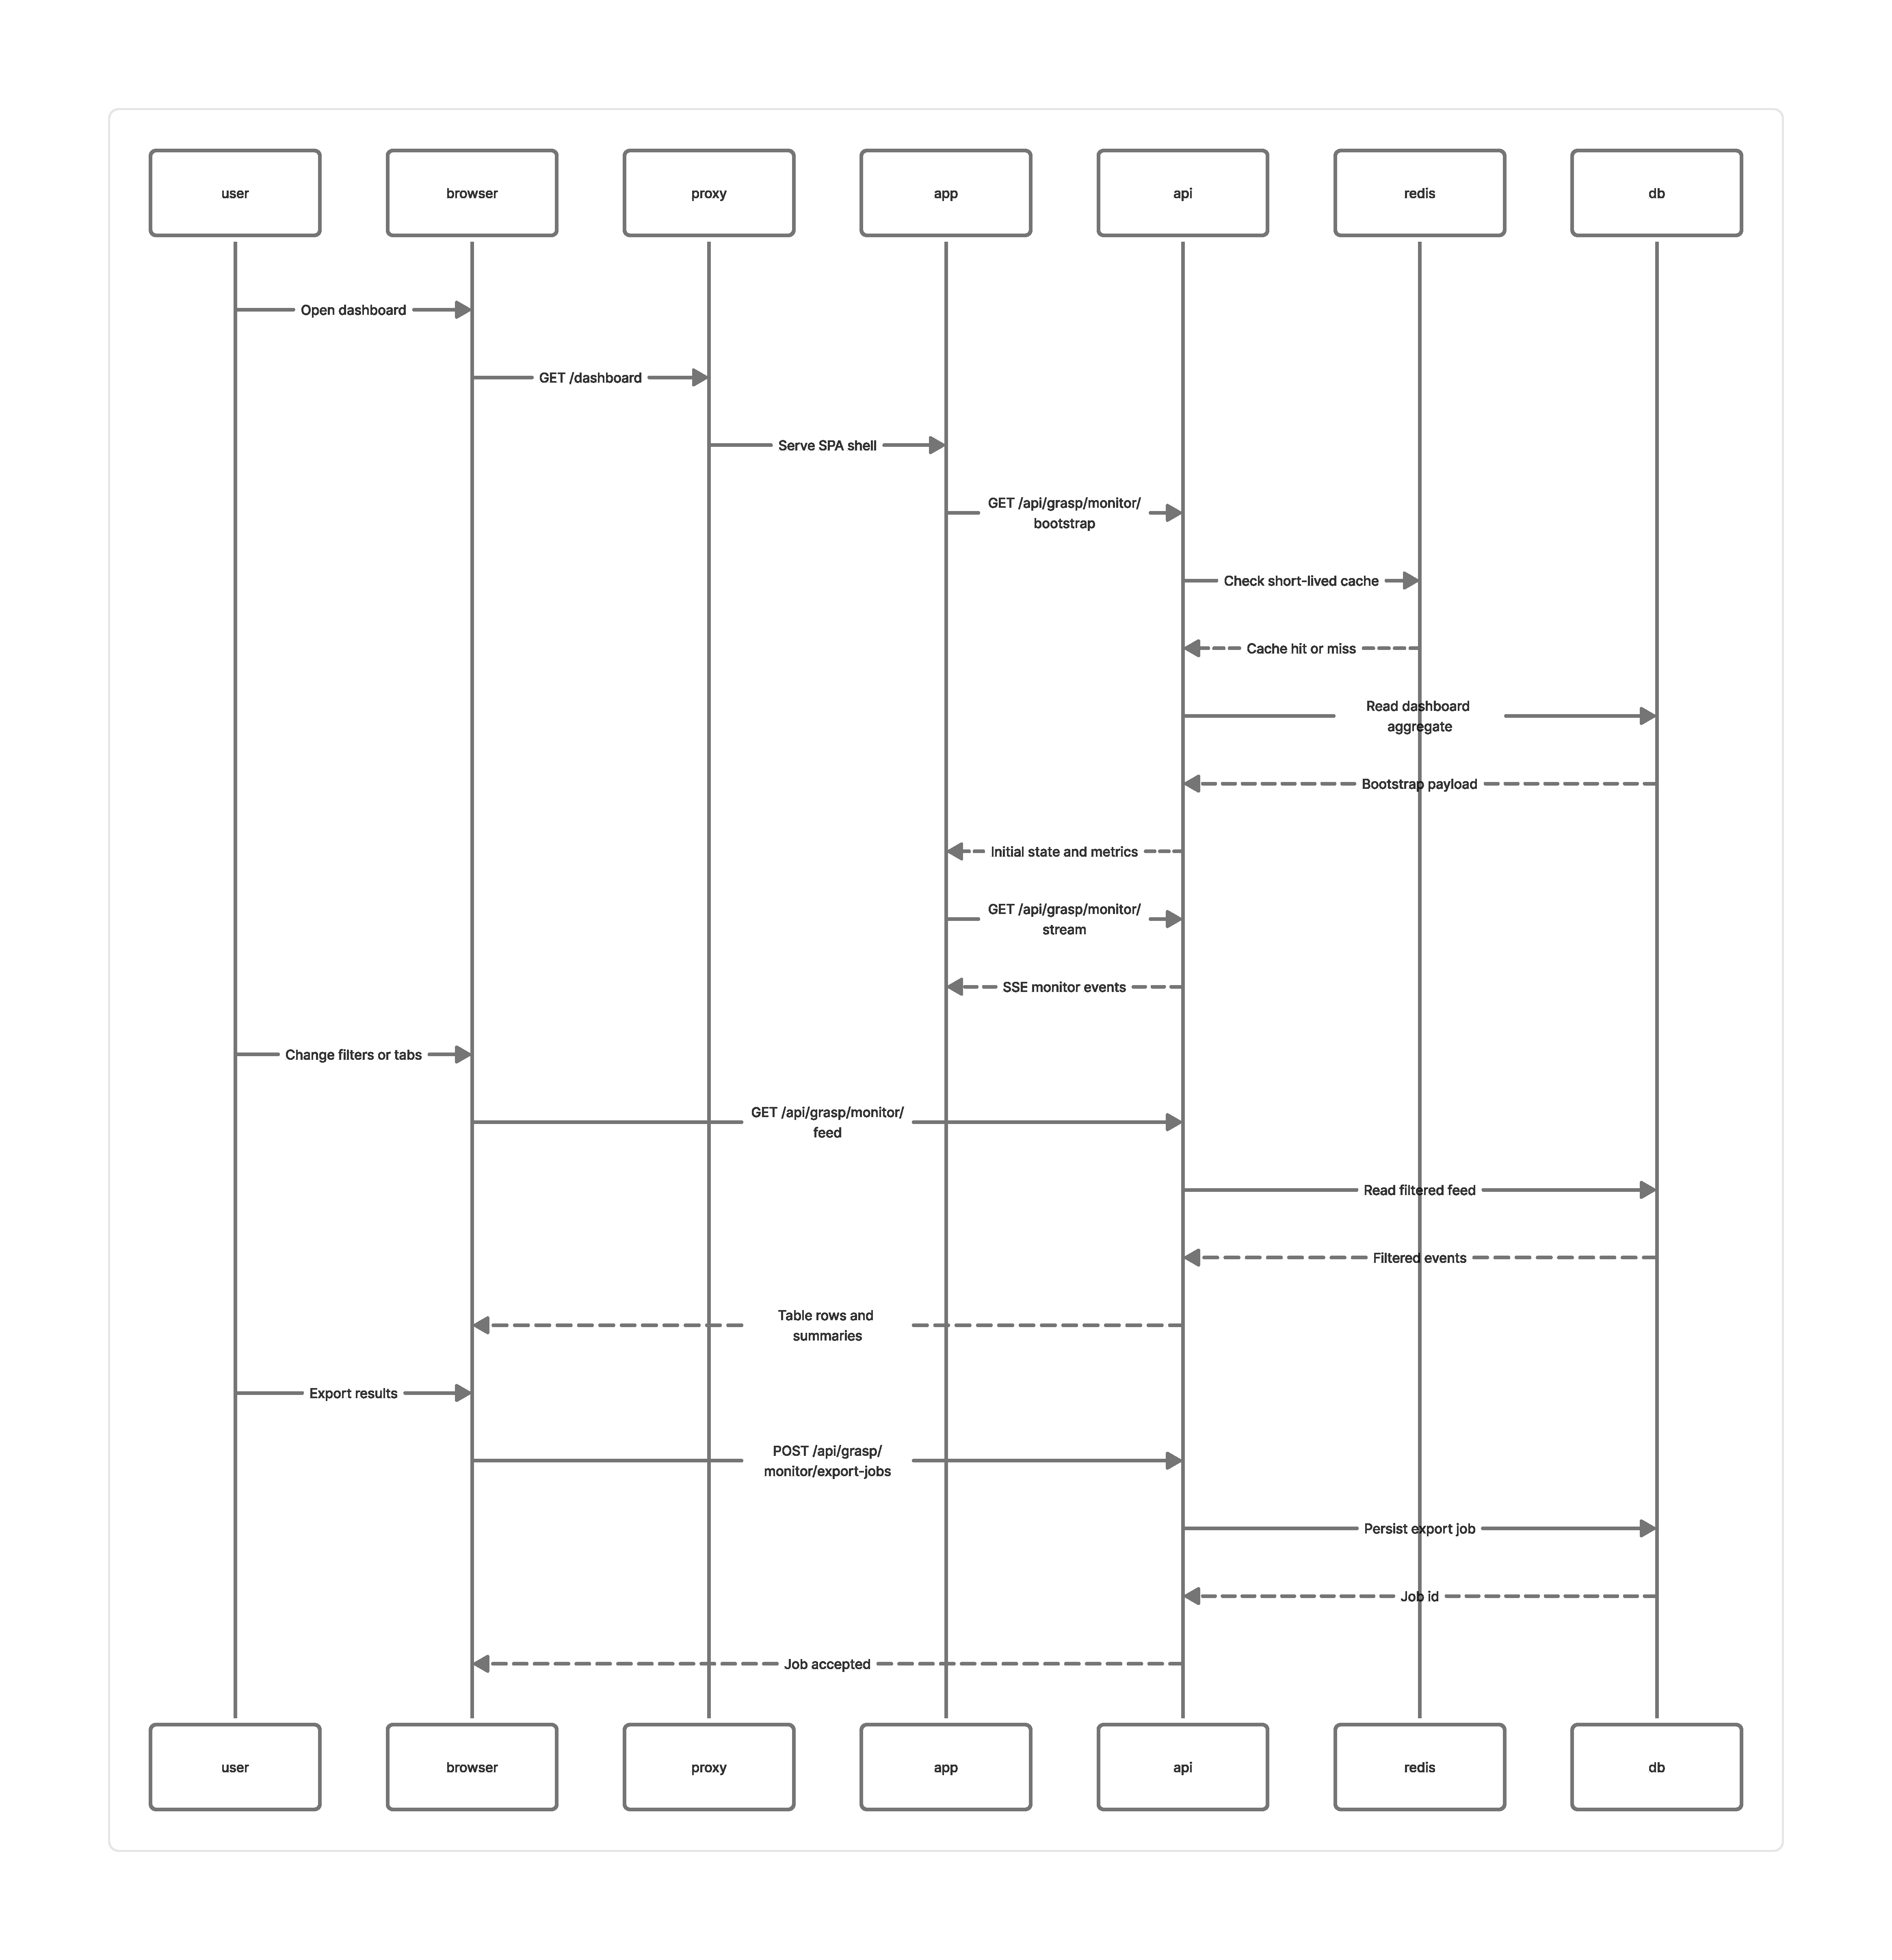
\includegraphics[width=.92\linewidth]{fig/gfshield/gfshield-front-flow.pdf}
  \caption{Diagrama do funcionamento do front-end.}
  \label{fig:app-front-flow}
\end{figure}

\begin{figure}[!htb]
  \centering
  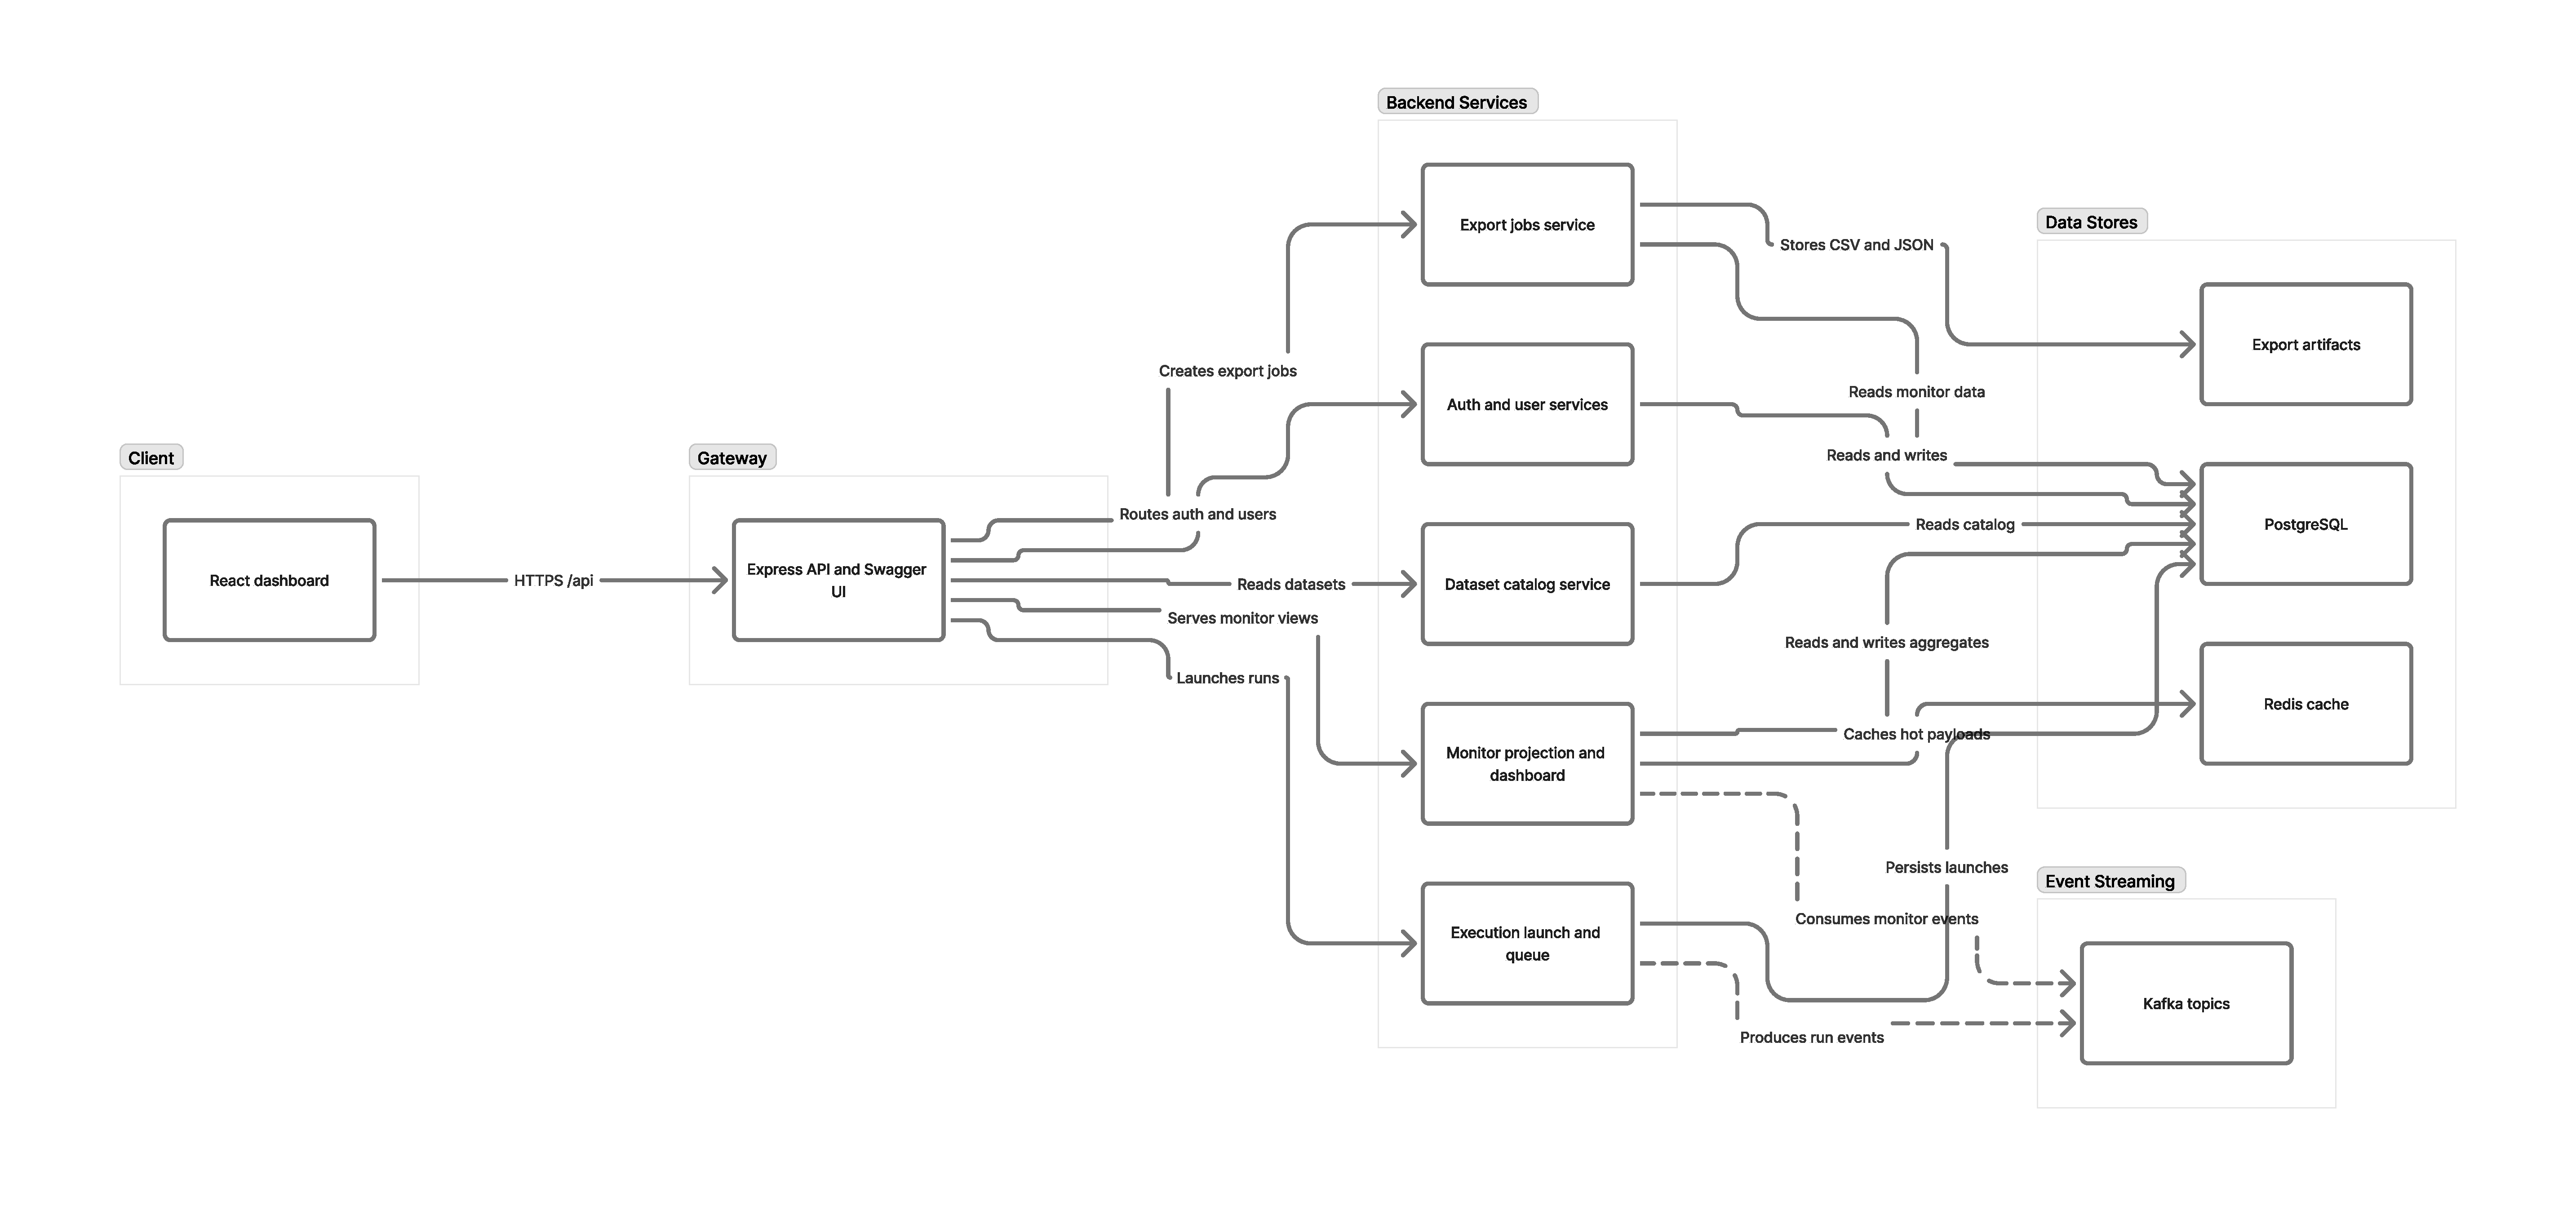
\includegraphics[width=.92\linewidth]{fig/gfshield/gfshield-backend-architecture.pdf}
  \caption{Diagrama da arquitetura do backend.}
  \label{fig:app-backend-architecture}
\end{figure}

\begin{figure}[!htb]
  \centering
  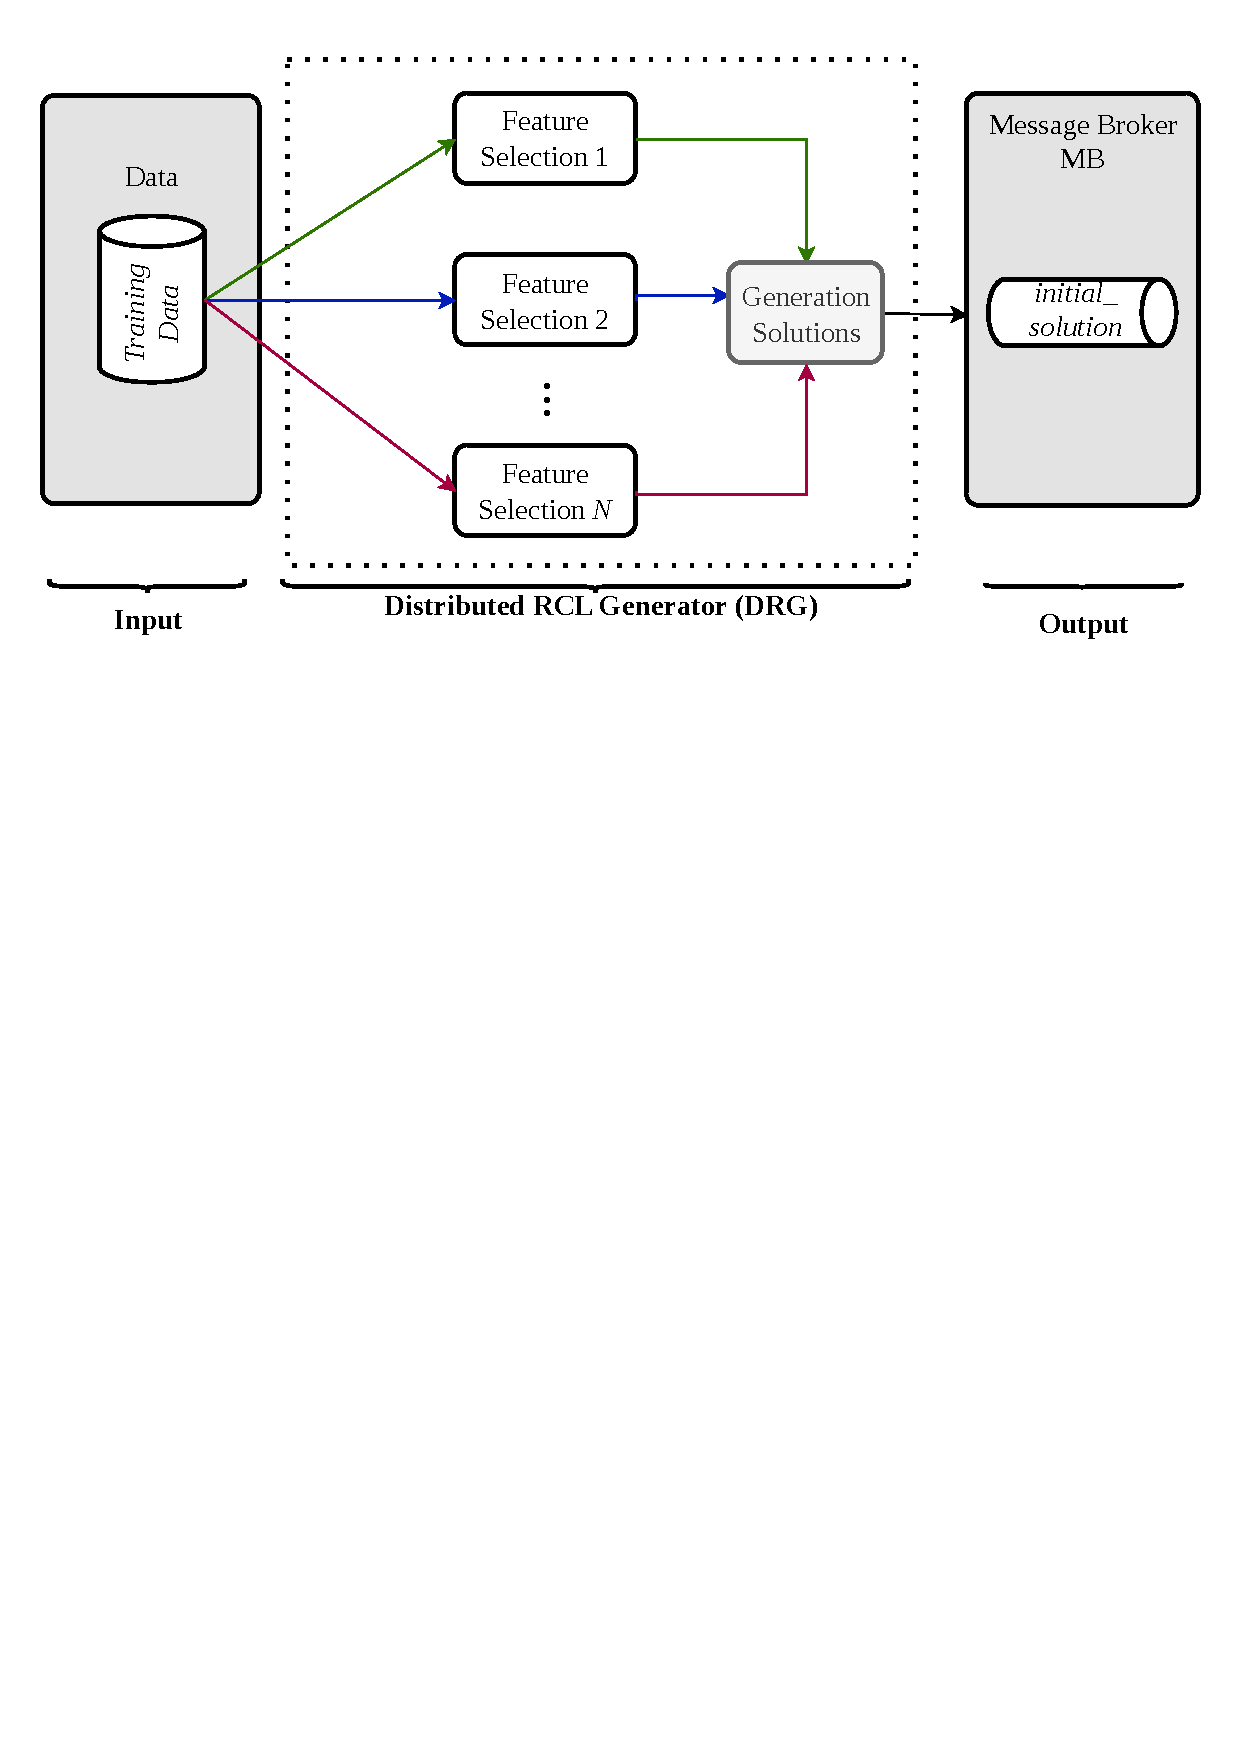
\includegraphics[width=.92\linewidth]{fig/gfshield/arquitetura-drg-generic.pdf}
  \caption{Versão genérica do DRG com entrada de dados abstrata.}
  \label{fig:app-drg-generic}
\end{figure}

\begin{figure}[!htb]
  \centering
  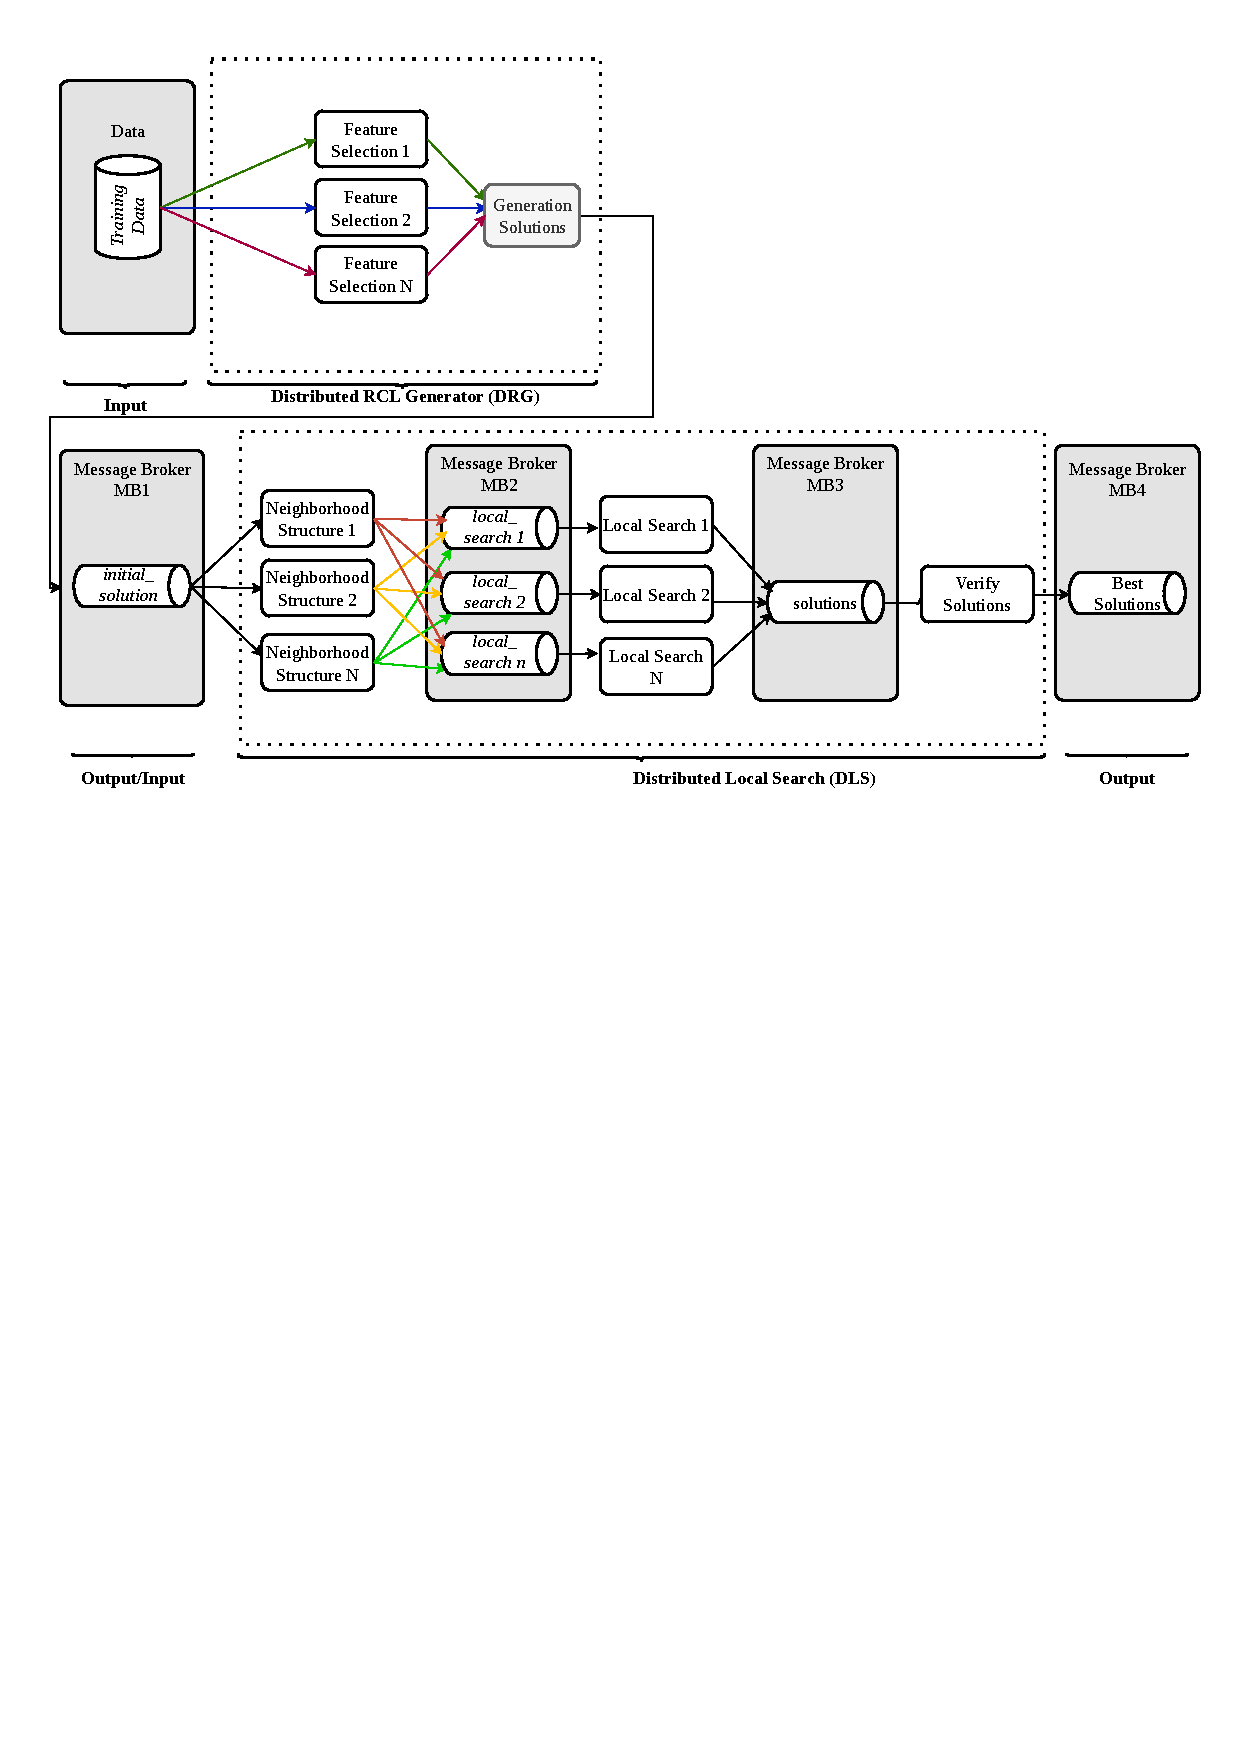
\includegraphics[width=.92\linewidth]{fig/gfshield/arquitetura-full-summary.pdf}
  \caption{Resumo visual da arquitetura completa do sistema.}
  \label{fig:app-architecture-summary}
\end{figure}

\end{apendicesenv}
